\PassOptionsToPackage{unicode}{hyperref}
\PassOptionsToPackage{naturalnames}{hyperref}
\documentclass[sigconf]{acmart}

% \usepackage{arxiv}

\usepackage[utf8]{inputenc} % allow utf-8 input
\usepackage[T1]{fontenc}    % use 8-bit T1 fonts
% \usepackage{hyperref}       % hyperlinks
\usepackage{url}            % simple URL typesetting
\usepackage{booktabs}       % professional-quality tables
\usepackage{amsfonts}       % blackboard math symbols
\usepackage{nicefrac}       % compact symbols for 1/2, etc.
\usepackage{microtype}      % microtypography
\usepackage{graphicx}       % images
\usepackage{mathtools}
\usepackage{parselines}
% \usepackage{biblatex}
\usepackage{verbatim}
\usepackage[ruled]{algorithm2e}

\AtBeginDocument{%
  \providecommand\BibTeX{{%
    \normalfont B\kern-0.5em{\scshape i\kern-0.25em b}\kern-0.8em\TeX}}}

%% Rights management information.  This information is sent to you
%% when you complete the rights form.  These commands have SAMPLE
%% values in them; it is your responsibility as an author to replace
%% the commands and values with those provided to you when you
%% complete the rights form.
\setcopyright{acmcopyright}
\copyrightyear{2020}
\acmYear{2020}
\acmDOI{X}

%% These commands are for a PROCEEDINGS abstract or paper.
\acmConference[KDD '20]{KDD '20}{X}{X}
\acmBooktitle{KDD '20}
\acmPrice{15.00}
\acmISBN{978-1-4503-XXXX-X/18/06}


\begin{document}
\title{Clustered Hierarchical Anomaly and Outlier Detection Algorithms}

\author{Thomas~J.~Howard~III}
\authornote{These authors contributed equally to this research.}
\email{thoward27@uri.edu}
\affiliation{%
  \institution{Computer Science and Statistics  University of Rhode Island}
  \city{Kingston}
  \state{RI}
  \postcode{02881}
}

\author{Najib~Ishaq}
\authornotemark[1]
\email{najib\_ishaq@zoho.com}
\affiliation{%
  \institution{Computer Science and Statistics  University of Rhode Island}
  \city{Kingston}
  \state{RI}
  \postcode{02881}
}

\author{Noah~M.~Daniels}
\email{noah\_daniels@uri.edu}
\affiliation{%
  \institution{Computer Science and Statistics  University of Rhode Island}
  \city{Kingston}
  \state{RI}
  \postcode{02881}
}

\renewcommand{\shortauthors}{Howard and Ishaq, et al.}

\begin{abstract}
In this paper we use CHESS for introspective anomaly detection.
Using the underlying clustering mechanism from CHESS, along with some manually supplied stopping criteria, we present strong evidence that CHESS is able to accurately map the underlying manifold of the data and that we are able to use this manifold and its inherent properties to successfully flag anomalous data.
We empirically demonstrate the effectiveness of our method using several synthetic data sets.
Finally, we explore some future opportunities that could greatly increase the scope of this work.
\end{abstract}

\begin{CCSXML}
<ccs2012>
   <concept>
       <concept_id>10010147.10010257</concept_id>
       <concept_desc>Computing methodologies~Machine learning</concept_desc>
       <concept_significance>500</concept_significance>
       </concept>
   <concept>
       <concept_id>10010147.10010257.10010258.10010260.10010229</concept_id>
       <concept_desc>Computing methodologies~Anomaly detection</concept_desc>
       <concept_significance>500</concept_significance>
       </concept>
 </ccs2012>
\end{CCSXML}

\ccsdesc[500]{Computing methodologies~Machine learning}
\ccsdesc[500]{Computing methodologies~Anomaly detection}

\keywords{
Anomaly Detection, Outlier Detection, Novelty Detection, Manifold Learning
}

\maketitle

\section{Introduction}
\label{sec:introduction}

Anomaly detection is difficult.
To determine if something deviates from normal, one must understand the normal, the abnormal, and the boundary between the two.

Normal data in the real-world are generated by some constrained generating phenomena.
Examples include:
\begin{itemize}
    \item biological evolution.
    \item stellar evolution.
    \item drug synthesis.
    \item network interactions.
\end{itemize}

Abnormal instances of data, which can be called \textit{outliers} or \textit{anomalies}, arise from such varied sources as:
\begin{itemize}
    \item errors in measurements and data collection.
    \item noise in data mimicking real outliers.
    \item blurry boundaries between abnormal and normal behaviour.
    \item normal behaviour evolving into abnormal behaviour.
    \item novel never-before-seen instances in data.
    \item adversarial attacks.
\end{itemize}

In this paper, we tackle this challenge using a novel Manifold Learning technique.
% TODO: and compare our performance against oft-used state-of-the-art anomaly-detection techniques.
We use CHESS~\cite{ishaq2019entropy} to build a clustering on the data.
We then build a graph from the leaf-clusters by creating edges between clusters that have overlapping volumes.
This process effectively learns the manifold that the data lie on.
Once we have learned a manifold, an anomaly is simply a point which does not fall on that manifold.

We test our methods on several synthetic datasets. These datasets all have the quality that the data occupy a non-linear, low-dimensional manifold in a high-dimensional embedding space.

We consider several different definitions for outliers and anomalies.
\begin{itemize}
    \item Since CHESS produces a distance-based clustering, we adapt several classical distance-based definitions of outliers.
    \item Since we have a clustering on our data, we can consider sparsely populated clusters to contain anomalies, thereby leveraging density-based definitions of outliers.
    \item Since we have a graph on our data, we have access to several graph-based methods for anomaly detection.
    \item Since search time is independent of the size of size of the data, we can use our method for novelty detection in streams of new data.
    \item Since the clustering can be live-updated, we can adapt to changing behaviour in new data.
\end{itemize}

All forms of clustering hitherto have suffered from one defect or another.
The most common deficiencies are: the effective treatment of high dimensionality, interpretability of results, and/or scalability to exponentially growing datasets ~\cite{rakesh_agrawal_automatic_1998}.
With CHESS, we have largely alleviate these problems while also uncoupling search-time from the size of the data being searched.
By defining edges via cluster-overlap, we build a graph representation of the manifold that the data occupy.
We use our knowledge of this manifold to guide the detection of anomalies, outliers and novelties.

% TODO: Add definitions: Anomaly, Outlier, Novelty, etc.

\section{Related Works}
\label{sec:realted_works}

In this section, we consider distance-based, clustering-based, and graph-based approaches.

\subsection{Clustering-Based Approaches}

Clustering data is universally centered around techniques for grouping points in a way that provides value.
This is done by assigning similar points to the same cluster.
Once these clusters are assigned, they can be used to check if there are any outliers present within the data.
The clusters can also be used to check if new points are anomalous.
For example, for any given point, one can check if it lies within, or near, any cluster; if not, the point can be marked as an anomaly.
To determine if the data contain any outliers, one can also examine the cardinality of various clusters and/or how dissimilar the clusters are to each other.
For example, if many clusters of large cardinality are present, along with relatively few clusters of very low cardinality, the clusters of low cardinality may contain outliers.

We summarize several major approaches to clustering data.
Note that there have been relatively few advancements in clustering techniques over the past decade~\cite{wang_progress_2019}. This may explain, or by attributable to, the observably poor performance, so far, of clustering data in high dimensional space~\cite{zhang_advancements_2013}.

\subsubsection{Distance-Based Clustering}

Distance-based clustering approaches rely on some distance measure to partition the data into some number of clusters.
Within this approach, the numbers of clusters and/or the sizes of clusters are predefined: either user-specified, or chosen at random~\cite{wang_progress_2019}.
Some examples of distance-based clustering are: 
K-Means~\cite{macqueen_methods_nodate}, 
PAM~\cite{kaufman_finding_nodate}, 
CLARANS~\cite{ng_efficient_nodate}, 
CLARA~\cite{kaufman_finding_nodate}, 
etc.

\subsubsection{Hierarchical Clustering}

Hierarchical clustering methods typically utilize a tree-like structure, where points are allocated into leaf nodes~\cite{wang_progress_2019}.
These tree-like structures can be created bottom-up (agglomerative clustering), or top-down (divisive clustering)~\cite{rakesh_agrawal_automatic_1998}.
The major drawback of these methods is the high cost of pairwise distance computations at each level of the tree.
Examples of hierarchical clustering include: 
MST~\cite{charles_zahn_graph_1971}, 
CURE~\cite{noauthor_cure:_nodate}, 
CHAMELEON~\cite{karypis_chameleon:_nodate}, 
etc.

\subsubsection{Density-Based Clustering}

Density-Based clustering methods rely on finding areas of high point-density separated by areas of low point-density.
These algorithms generally do not work well when normal data are sparse.
Some examples of density-based clustering algorithms are: 
DBSCAN~\cite{ester_density-based_nodate}, 
DENCLUE~\cite{Hinneburg1998Effic-5816}, 
etc.

\subsubsection{Grid-Based Clustering}

Grid-based clustering works via segmenting the entire space into a finite number of cells and then iterating over the cells to find regions of higher density.
Utilizing the grid structure for clustering means that these algorithms typically scale better to larger datasets.
Some examples of grid-based clustering: 
STING~\cite{sting:wang}, 
Wavecluster~\cite{Wavecluster:Sheikholeslami:2000}, 
DCluster,  % Paper does not exist????
CLIQUE~\cite{rakesh_agrawal_automatic_1998}, 
etc.

\subsection{Distanced-Based Approaches}

Distance-based methods attempt to find anomalous points via distance comparisons.
These methods largely employ k-Nearest Neighbors as their substrate~\cite{wang_progress_2019}.
They proceed in the following, slightly different, ways:

\begin{enumerate}
    \item Points with less than $p$ other points within a distance $d$ are outliers.
    \item The top $n$ points whose distances to their $k^{th}$-nearest neighbor are the greatest are outliers.
    \item The top $n$ points whose average distances to their $k^{th}$-nearest neighbor are the greatest are outliers.
\end{enumerate}


% CLIQUE Summary
\begin{comment}
CLIQUE scales linearly with input records, but does identify subspaces within the original dataset.
CLIQUE clusters based on subspaces it identifies via density estimates, it does not cluster in the full dimensionality of the input data.
This seems to be the premonition of manifold finding.
Restricted look to subspaces of the original set, not fictitious subspaces dreamed up via techniques such as Principle Component Analysis.
CLIQUE finds areas of higher density, which are the clusters.
Begins by partitioning the full space into units then estimates density within that cell.
All clusters are axis-parallel hyper-rectangles. Each cluster is a union of adjacent dense cells.
Compact representation is then found by covering the cluster with a minimal number of maximal, possibly overlapping rectangles and describing the cluster as the union of said rectangles.
CLIQUE is also tolerant to incomplete data points.
Requires density threshold and number of intervals over the full space as parameters.
Categorical data is ordered arbitrarily, with an empty interval placed in-between ever pair.
Is deterministic, always yields the same results.
Runs in $O(c^k + m k)$ where $c$ is some constant, $k$ is the dimensionality, and $m$ is the number of points.
Tested on dimensionality up to 50.
In experiments run for this paper, BIRCH failed starting at 20 dimensions, DBSCAN at 8, CLIQUE made it to 50 without failure.
\cite{rakesh_agrawal_automatic_1998}
\end{comment}

\section{Methods}
\label{sec:methods}

For this work we have applied a multitude of different Distance-Based, Density-Based, and Graph-Based, approaches to detect anomalous and outlying points/clusters.
In this section, we detail the specific algorithms employed from these various categories.

\subsection{Distance-Based Outliers}

\begin{algorithm}
\DontPrintSemicolon
\SetAlgoLined
\KwData{manifold, depth}
\KwResult{scores}
 $scores \leftarrow \{\}$\;
 $d \leftarrow depth$\;
 \ForAll{cluster $c \in$ manifold.graph(d).clusters}{
  \ForAll{$p \in c.points$}{
   $scores[p] \leftarrow |c|$
  }
 }
 normalize(scores)\;
 \ForAll{$p \in scores$}{$scores[p] \leftarrow 1-p$}
 \caption{Cluster Cardinality}
 \label{alg-cc}
\end{algorithm}

\begin{algorithm}
\DontPrintSemicolon
\SetAlgoLined
\KwData{manifold,depth}
\KwResult{scores}
 $scores \leftarrow \{\}$\;
 $d \leftarrow depth$\;
 \For{$d \in 1\cdots$ depth}{
  \ForAll{cluster $c \in $manifold.graph(d).clusters}{
    \ForAll{point $p \in c$}{
     $scores[p] \leftarrow \frac{|c.parent|}{|c|\times d}$
    }
  }
 }
 normalize(scores)\;
 \caption{Hierarchical}
 \label{alg-hierarchical}
\end{algorithm}


\begin{algorithm}
\DontPrintSemicolon
\SetAlgoLined
\KwData{manifold,depth,k}
\KwResult{scores}
 $scores \leftarrow \{\}$\;
 $d \leftarrow $ depth\;
 $g \leftarrow $ manifold.graph(d).clusters\;
 \ForAll{cluster $c \in g$}{
  $v \leftarrow |\{c' \in g | \delta(c,c') \le k\}|$\;
  \ForAll{$p \in c$}{
   scores[p] $\leftarrow v$\;
  }
 }
 normalize(scores)\;
 \ForAll{$p \in scores$}{$scores[p] \leftarrow 1-p$}
 \caption{k-Neighborhood}
 \label{alg-kneighborhood}
\end{algorithm}


% Must cite outrank paper for this one

\begin{algorithm}
\DontPrintSemicolon
\SetAlgoLined
\KwData{manifold,depth}
\KwResult{scores}
 $scores \leftarrow \{\}$\;
 $d \leftarrow $ depth\;
 $g \leftarrow $ manifold.graph(d).components\;
 \ForAll{component $k \in g$}{
  visits $\leftarrow$ outrank(k)\;
  \ForAll{cluster $c \in k$}{
   $v \leftarrow $visits[c]\;
   \ForAll{$p \in c$}{
    scores[p] $\leftarrow v$\;
   }
  }
 }
 normalize(scores)\;
 \ForAll{$p \in scores$}{$scores[p] \leftarrow 1-p$}
 \caption{Random Walk}
 \label{alg-rw}
\end{algorithm}

\begin{algorithm}
\DontPrintSemicolon
\SetAlgoLined
\KwData{manifold, depth}
\KwResult{scores}
 $scores \leftarrow \{\}$\;
 $d \leftarrow depth$\;
 \ForAll{component $k \in$ manifold.graph(d).components}{
  \ForAll{cluster $c \in k$}{
   \ForAll{$p \in c$}{
    scores[p] $\leftarrow |k|$
   }
  }
 }
 normalize(scores)\;
 \ForAll{$p \in scores$}{$scores[p] \leftarrow 1-p$}
 \caption{Subgraph Cardinality}
 \label{alg-sgc}
\end{algorithm}

\begin{enumerate}
    \item Sort all points $p \in \mathbb{P}$, where $\mathbb{P}$ is the data, by $f \equiv |B_D(p, r)|$ in ascending order.
    \begin{itemize}
        \item If needed, increase $r$ to break ties.
        \item The points with the smallest values of $f$ are the outliers.
    \end{itemize}
    \item Sort all points $p \in \mathbb{P}$ in descending order by the distance to their $k^{th}$ nearest neighbor.
    \begin{itemize}
        \item Consider how this distance changes as $k$ in increased.
        \item The points with the highest such distances are the outliers.
    \end{itemize}
\end{enumerate}

\subsection{Hierarchical-Clustering-Based Outliers}

\begin{enumerate}
    \item For a $parent$ cluster and its $left$ and $right$ child-clusters (assume without loss of generality that $|left| \leq |right|)$ define $f \equiv \frac{|left|}{|parent|}$. If $f \ll 0.5$ then points in the $|left|$ cluster are outliers.
    \begin{itemize}
        \item Use this definition recursively down the tree. The number of levels in the tree at which a point is labelled an outlier gives us a measure of the ``anomalousness'' of that point.
    \end{itemize}
\end{enumerate}

\subsection{Graph-Based Outliers}

\begin{enumerate}
    \item The Outrank algorithm~\cite{moonesinghe_outrank:_2008} i.e. on a given graph-representation of data, initiate a random walk. The clusters that are visited least often are the outlier clusters.
    \item Define the ``k-neighborhood'' of a clusters $c$ as the clusters that can be reached from $c$ in $k$ steps. Investigate how $|k-neighborhood|$ increases as $k$ in increased.
    \begin{itemize}
        \item $|k-neighborhood|$ should increase by $k^d$ where $d$ is \textit{local fractal dimension} of the data at the length-scale of the radii of the clusters that form the graph.
        \item If the increase in $|k-neighborhood|$ of a cluster $c$ does not keep pace with $k^d$ as $k$ is increased then $c$ can be considered an outlier cluster.
    \end{itemize}
    \item Consider the connected components of the graph at a depth in the tree just before the graph shatters into many small components or isolated clusters.
    \begin{itemize}
        \item If a component contains too few points/clusters then those points/clusters can be considered outliers.
        \item If a small component is connected to a larger component with a small number of edges then the smaller component may contain outliers.
    \end{itemize}
\end{enumerate}

Due to the wide range of possible measurements for ``anomalousness'' from our methods, we normalize our measurements.

\subsection{Normalization Methods}

\begin{enumerate}
    \item Min-Max Scaling:
    \begin{gather}
        x^{\prime} = \frac{x - x_{min}}{x_{max} - x_{min}}
        \label{sec:methods:min-max-normalizationn}
    \end{gather}
    
    \item Mean-Scaling:
    \begin{gather}
        x^{\prime} = \frac{x - \overline{x}}{x_{max} - x_{min}}
        \label{sec:methods:mean-scaling}
    \end{gather}
    
    \item z-Score Standardization:
    \begin{gather}
        x^{\prime} = \frac{x - \overline{x}}{\sigma}
        \label{sec:methods:z-score}
    \end{gather}

\end{enumerate}

\section{Results}
\label{sec:results}

We have implemented and tested our methods on 26 different real-world datasets.
The vast majority of datasets studied were sourced from Outlier Detection Datasets (ODDS), which provided clear labels for normal and anomalous behavior.
We examine the effectiveness of our methods by their ability to identify these outliers.

Figure~\ref{results:datasets} shows % TODO
We chose to use so many different real world datasets to ensure that our methods could generalize to many target audiences.

\begin{figure*}[!t]
\centering
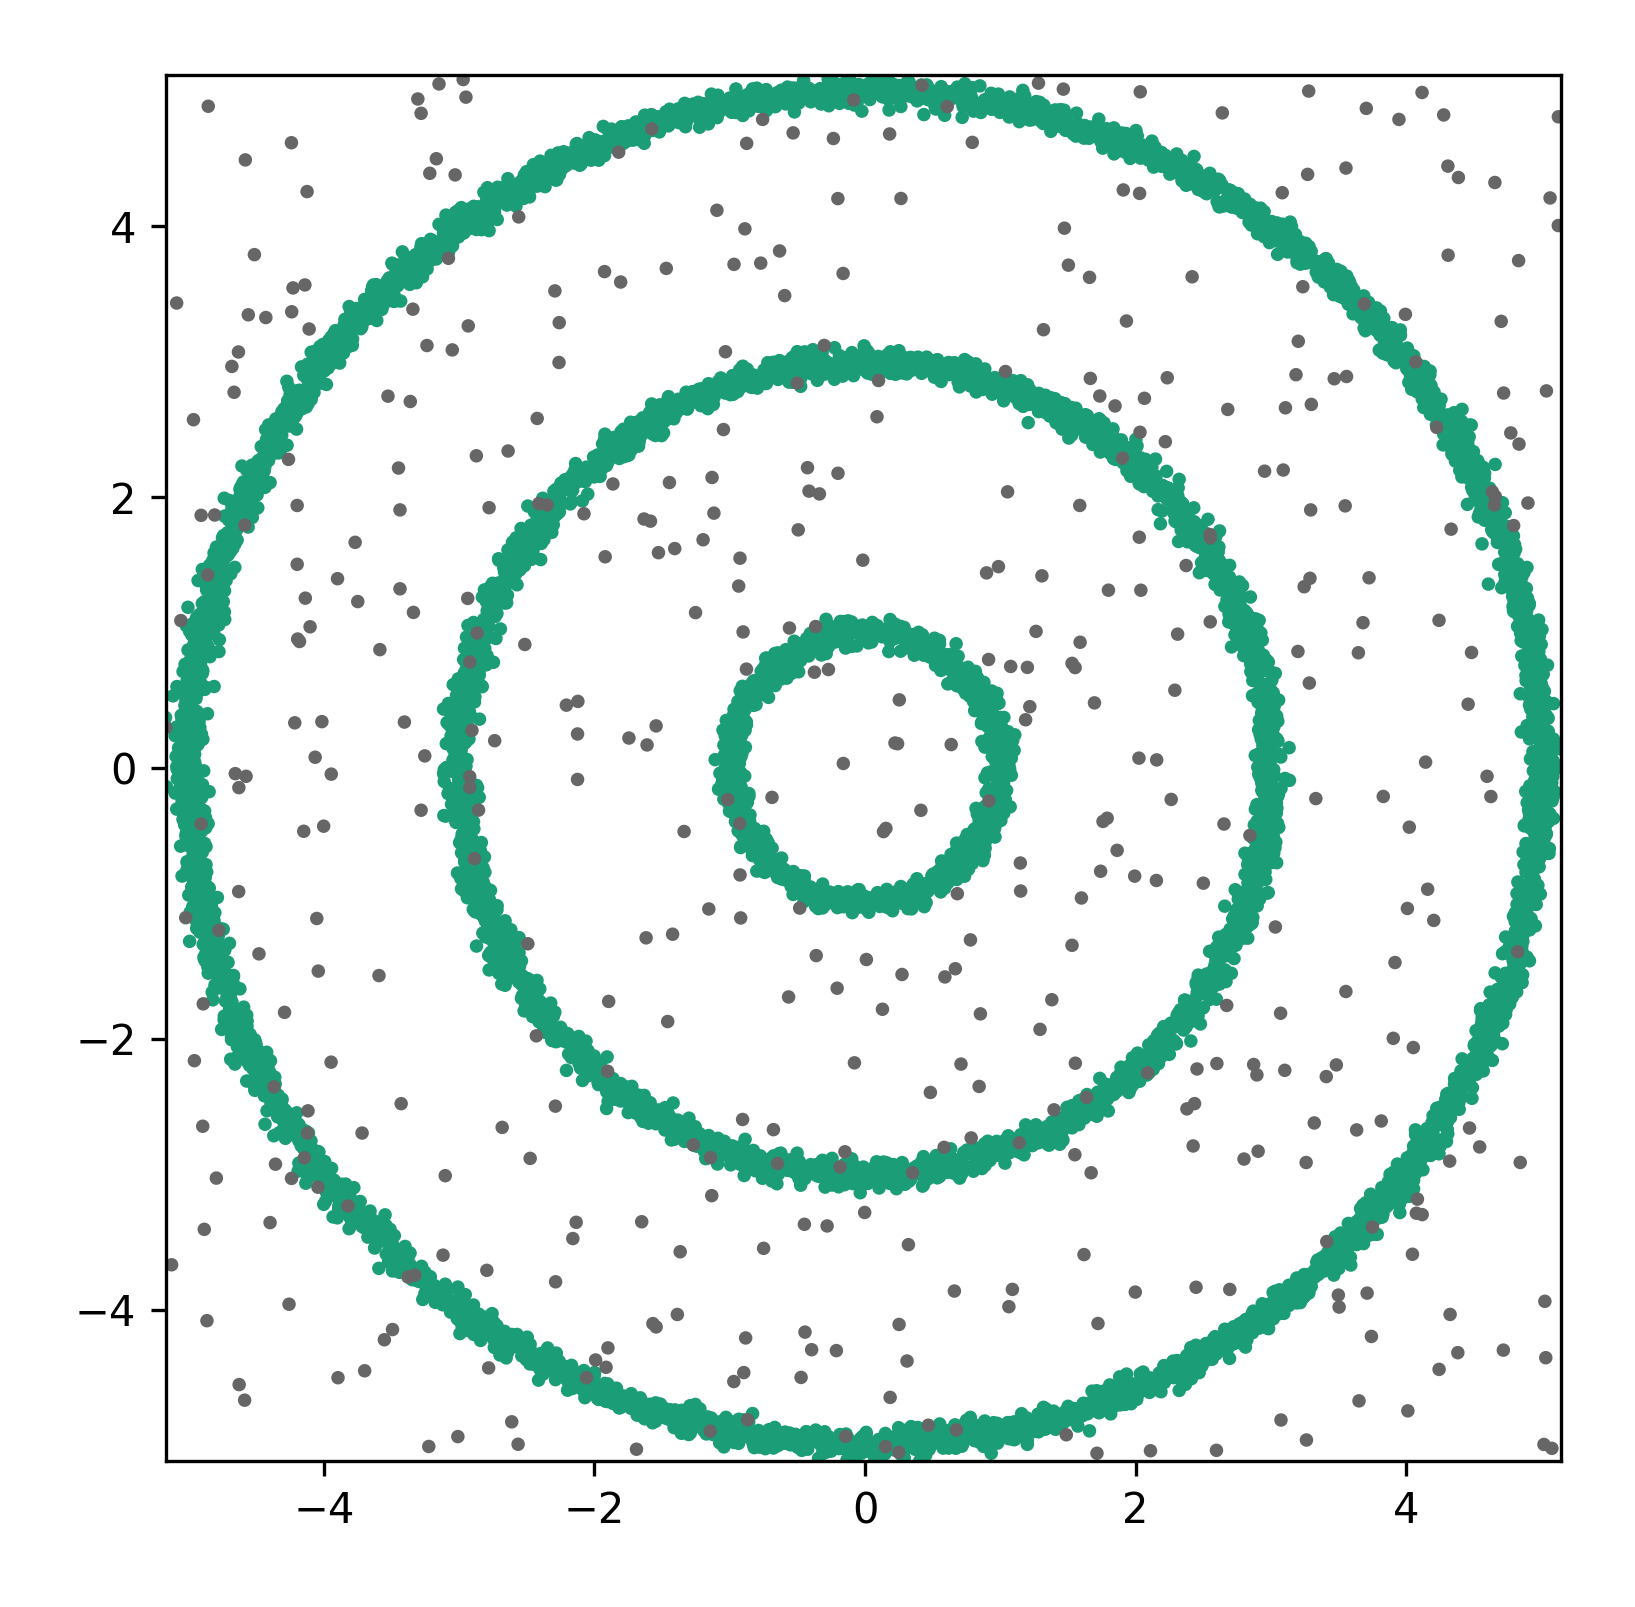
\includegraphics[width=2.5in]{static/bullseye.png}
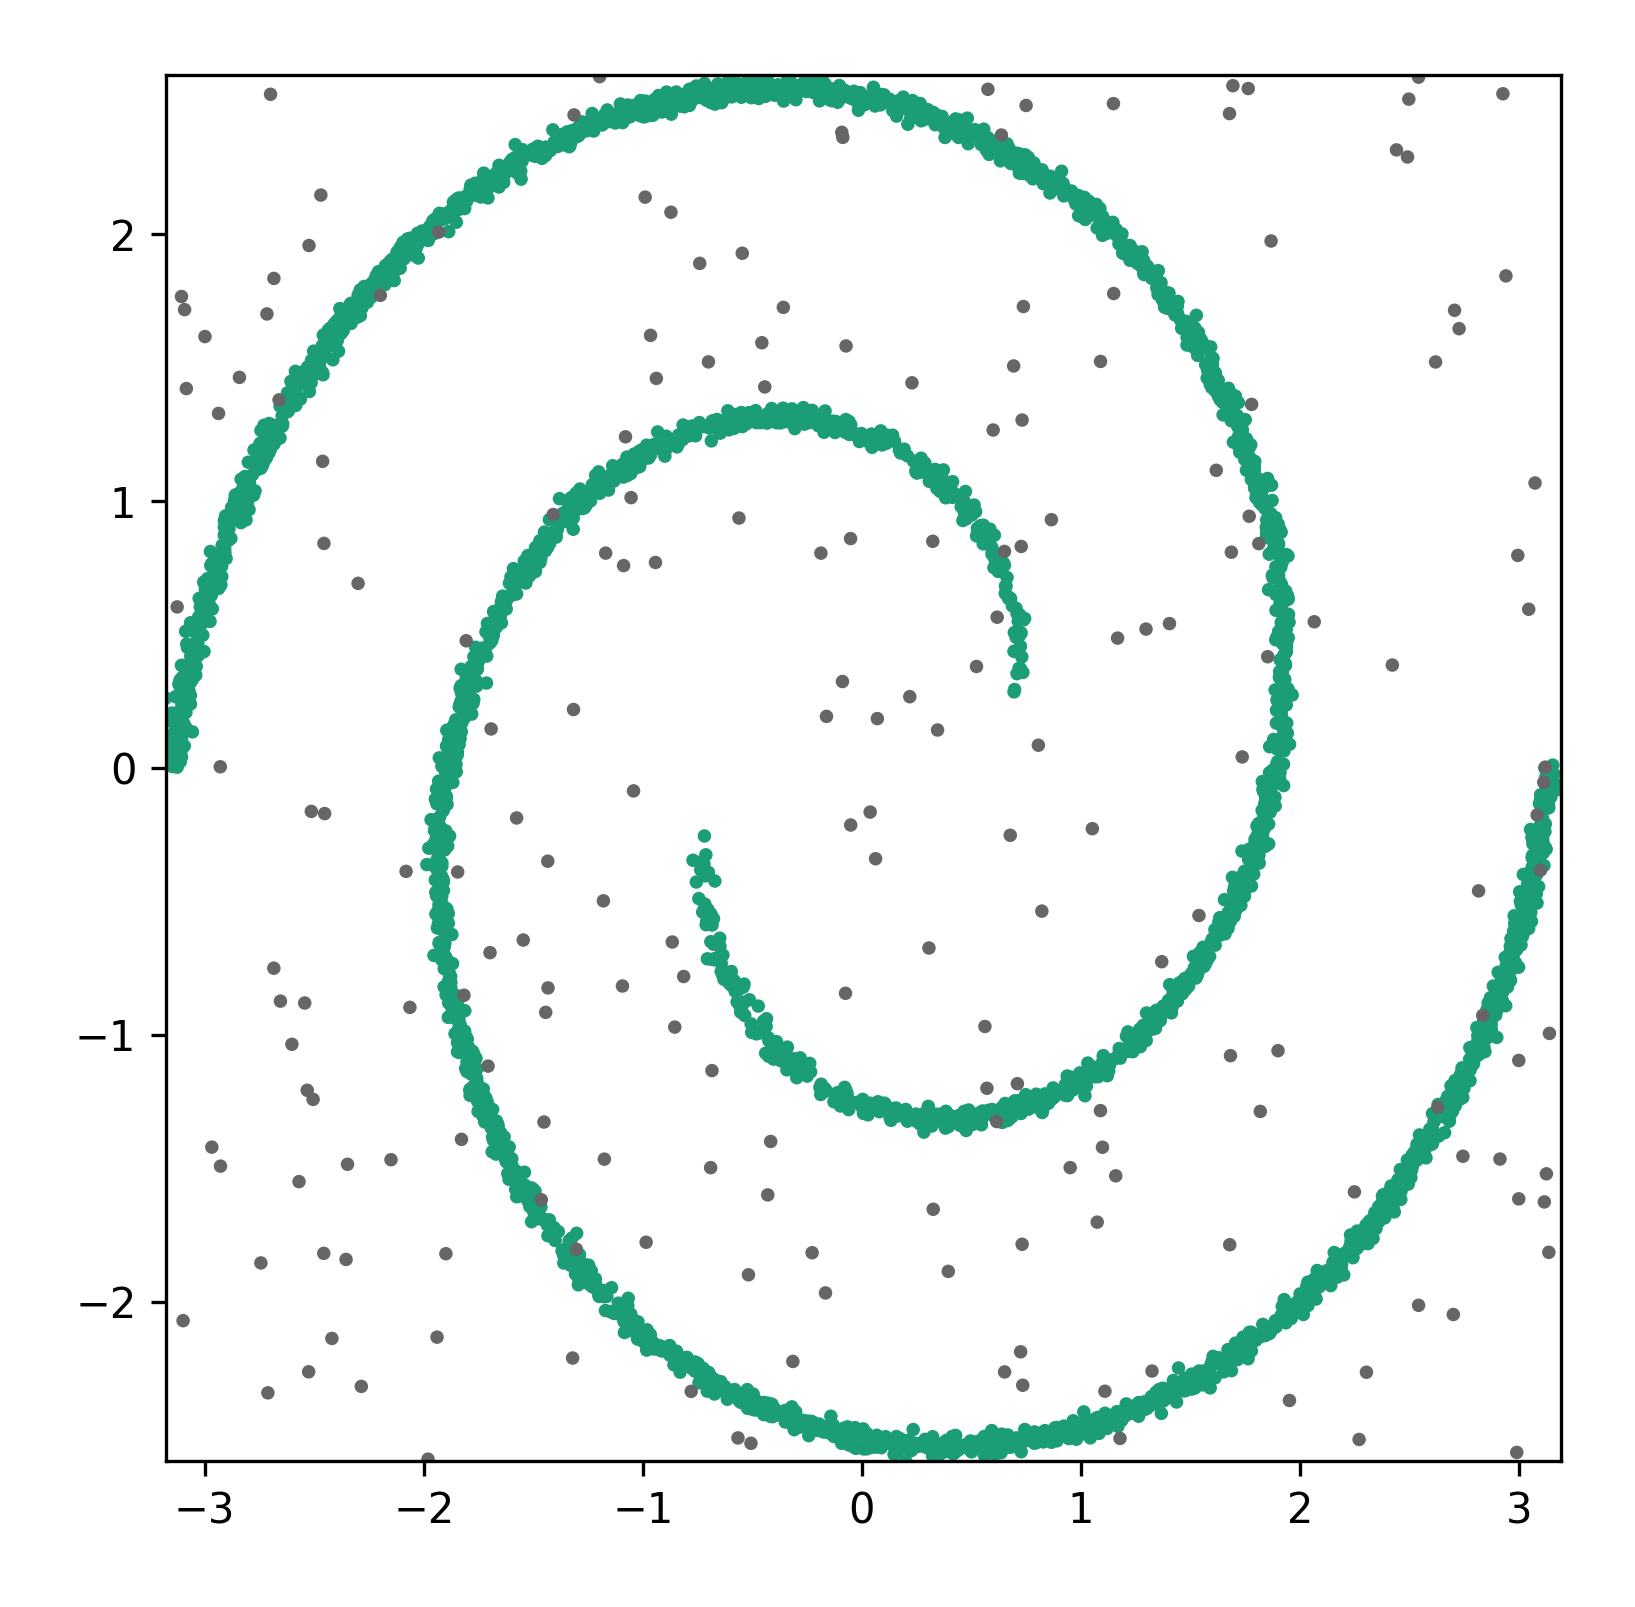
\includegraphics[width=2.5in]{static/spiral.png}
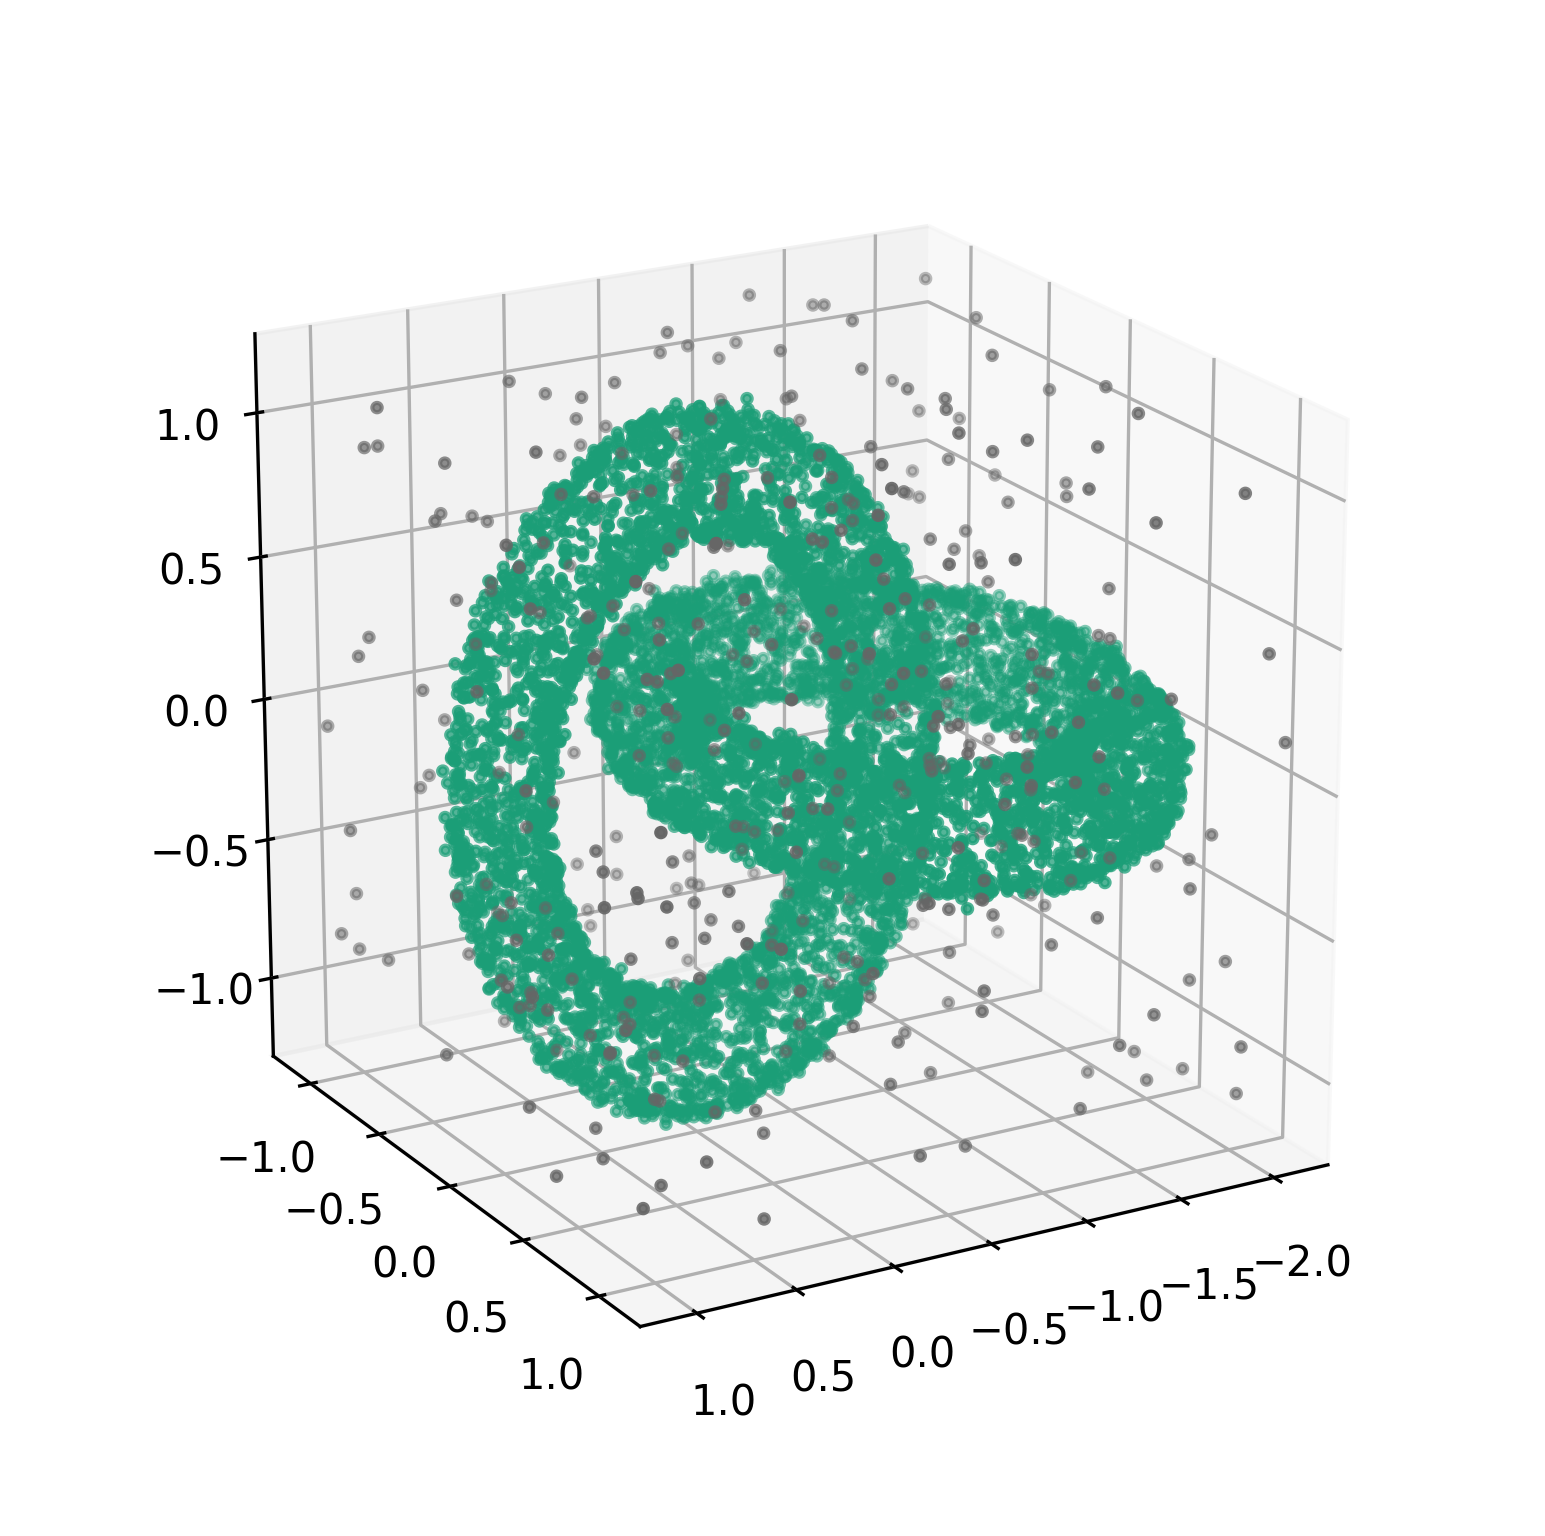
\includegraphics[width=3in]{static/interlocking_tori.png}
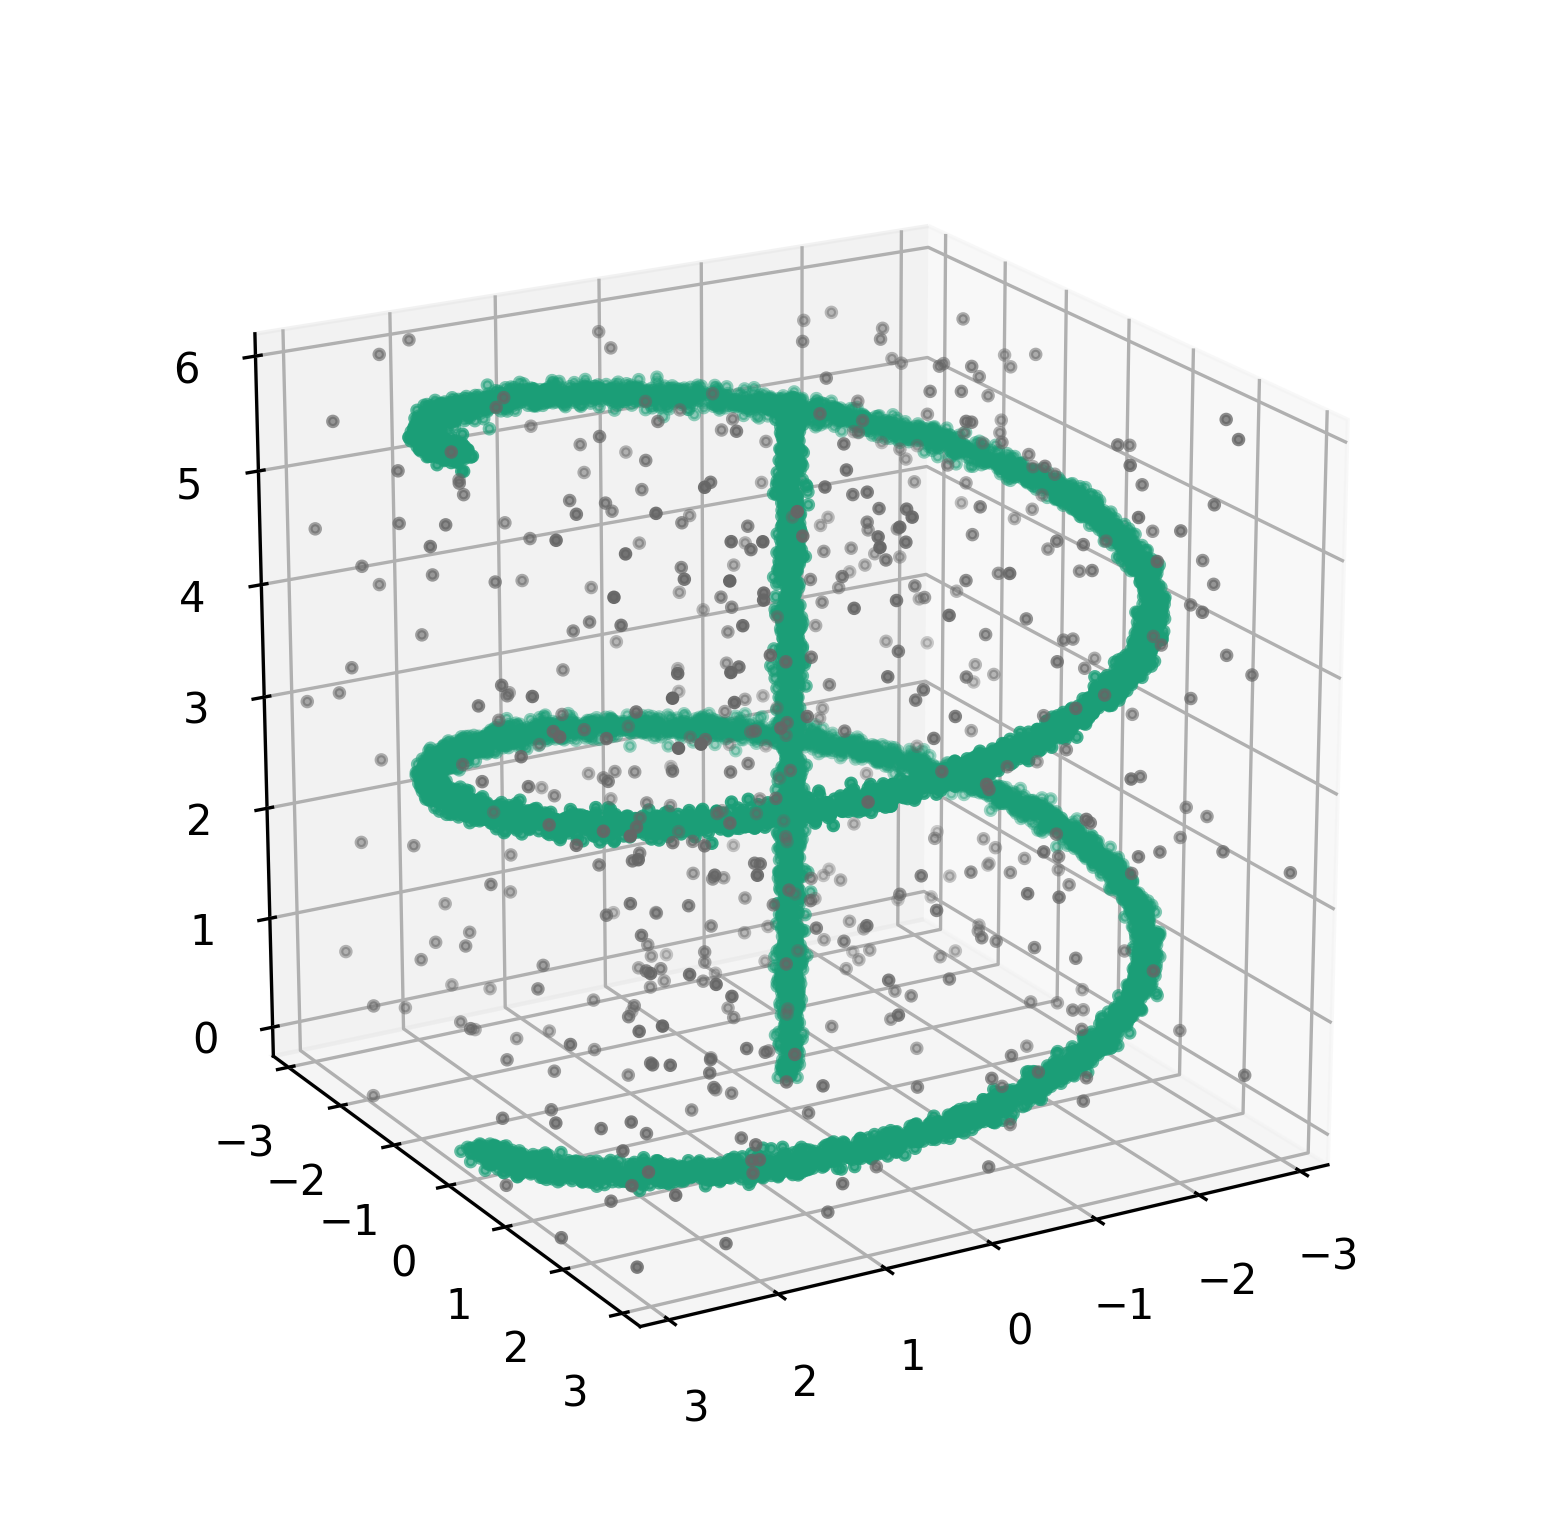
\includegraphics[width=3in]{static/skewer.png}
\caption{The Bullseye (top-left), Spiral (top-right), Interlocking Tori (bottom-left) and Skewer (bottom-left) datasets.}
\label{results:datasets}
\end{figure*}

For each dataset, we clustered using Manhattan, Euclidean, and Cosine distance functions.
Additionally, for this work, we allowed CLAM to cluster down until the manifold had thoroughly shattered.
We then iterated over all depths to compute the area under the ROC-Curve.

After computing anomalousness scores, we normalized each metric to a $[0, 1]$ range.
For each dataset, we present a confusion matrix, a ROC curve, and the area under the ROC curve for a sample of optimal depths. 
To demonstrate our methods are not overly-sensitive to depth we present all metrics in a 5-depth wide window.

Table~\ref{results:table} lists % TODO

\begin{table*}[!t]
\renewcommand{\arraystretch}{1.3}
\caption{Comparison of CHAODA with state-of-the-art algorithms}
\label{results:table}
\centering
\begin{tabular}{|c|c|c|c|c|c|c|c|c|c|c|c|c|c|c|c|}
\hline
{\textbf{Dataset}} & {\textbf{Metric}} & {\textbf{Method}} & \multicolumn{3}{c|}{\textbf{AUC ROC}} & \multicolumn{10}{c|}{\textbf{ }} \\
\hline
 &  &  & d - 2 & d & d + 2 &  &  &  &  &  &  &  &  &  & \\
\hline
\bfseries lympho & \bfseries cosine & \bfseries cluster\_cardinality & 0.926 & 0.949 & 0.838 &  &  &  &  &  &  &  &  &  & \\ 
\hline
\bfseries lympho & \bfseries cosine & \bfseries hierarchical & 0.927 & 0.940 & 0.938 &  &  &  &  &  &  &  &  &  & \\ 
\hline
\bfseries lympho & \bfseries cosine & \bfseries k\_neighborhood & 0.500 & 0.888 & 0.725 &  &  &  &  &  &  &  &  &  & \\ 
\hline
\bfseries lympho & \bfseries cosine & \bfseries random\_walk & 0.803 & 0.964 & 0.952 &  &  &  &  &  &  &  &  &  & \\ 
\hline
\bfseries lympho & \bfseries cosine & \bfseries subgraph\_cardinality & 0.583 & 0.739 & 0.729 &  &  &  &  &  &  &  &  &  & \\ 
\hline
\bfseries lympho & \bfseries euclidean & \bfseries cluster\_cardinality & 0.672 & 0.904 & 0.887 &  &  &  &  &  &  &  &  &  & \\ 
\hline
\bfseries lympho & \bfseries euclidean & \bfseries hierarchical & 0.672 & 0.869 & 0.863 &  &  &  &  &  &  &  &  &  & \\ 
\hline
\bfseries lympho & \bfseries euclidean & \bfseries k\_neighborhood & 0.500 & 0.573 & 0.500 &  &  &  &  &  &  &  &  &  & \\ 
\hline
\bfseries lympho & \bfseries euclidean & \bfseries random\_walk & 0.704 & 0.783 & 0.692 &  &  &  &  &  &  &  &  &  & \\ 
\hline
\bfseries lympho & \bfseries euclidean & \bfseries subgraph\_cardinality & 0.500 & 0.500 & 0.500 &  &  &  &  &  &  &  &  &  & \\ 
\hline
\bfseries lympho & \bfseries manhattan & \bfseries cluster\_cardinality & 0.793 & 0.965 & 0.962 &  &  &  &  &  &  &  &  &  & \\ 
\hline
\bfseries lympho & \bfseries manhattan & \bfseries hierarchical & 0.935 & 0.965 & 0.955 &  &  &  &  &  &  &  &  &  & \\ 
\hline
\bfseries lympho & \bfseries manhattan & \bfseries k\_neighborhood & 0.648 & 0.818 & 0.818 &  &  &  &  &  &  &  &  &  & \\ 
\hline
\bfseries lympho & \bfseries manhattan & \bfseries random\_walk & 0.763 & 0.960 & 0.955 &  &  &  &  &  &  &  &  &  & \\ 
\hline
\bfseries lympho & \bfseries manhattan & \bfseries subgraph\_cardinality & 0.583 & 0.663 & 0.660 &  &  &  &  &  &  &  &  &  & \\ 
\hline

\end{tabular}
\end{table*}

\begin{figure*}[!t]
\centering
% Annthyroid
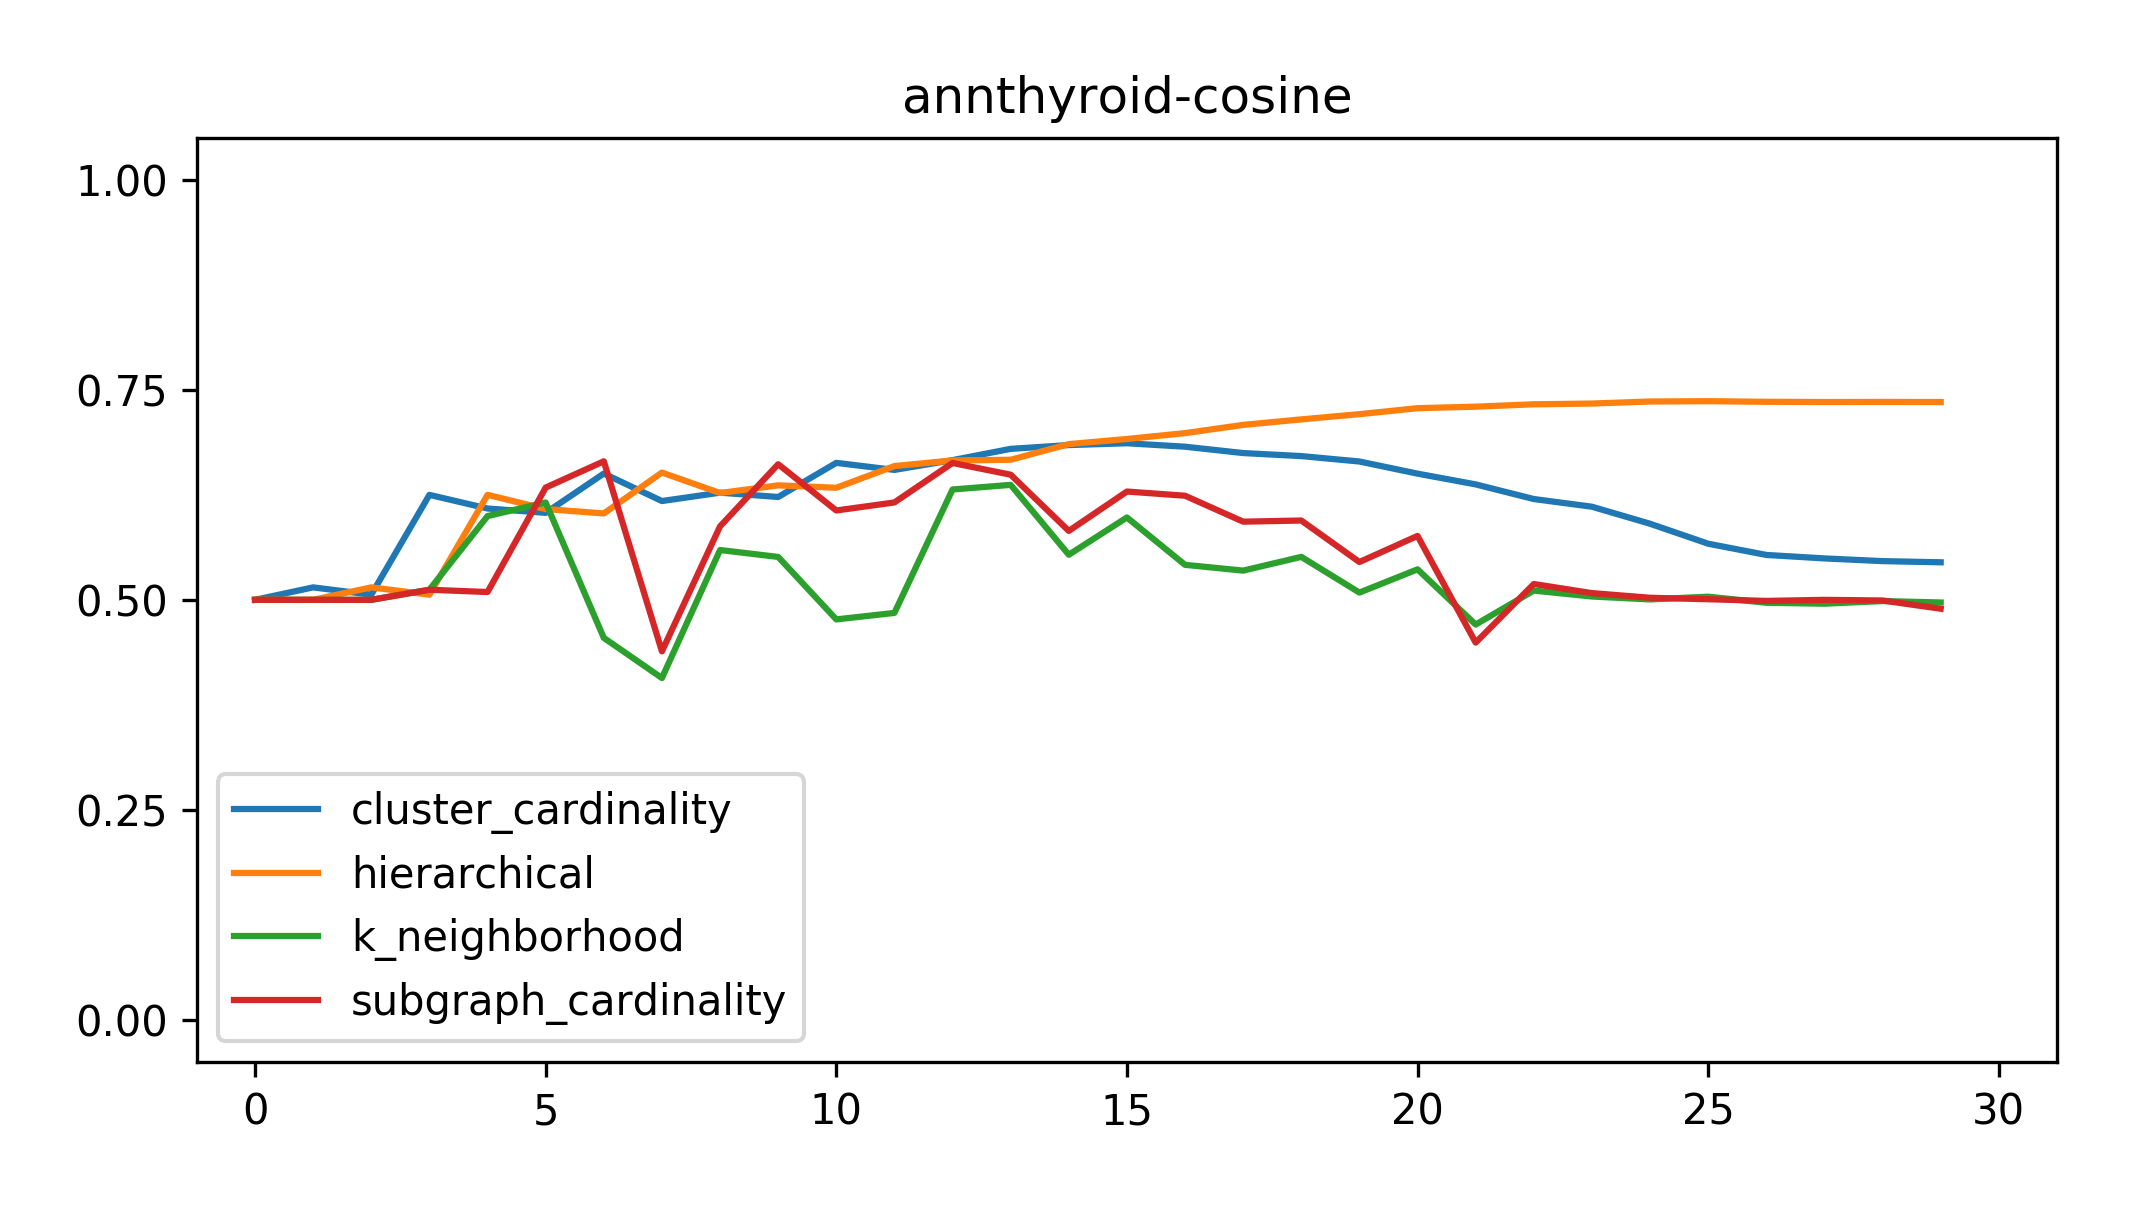
\includegraphics[width=2.2in]{kdd/static/auc_vs_depth/annthyroid-cosine.png}
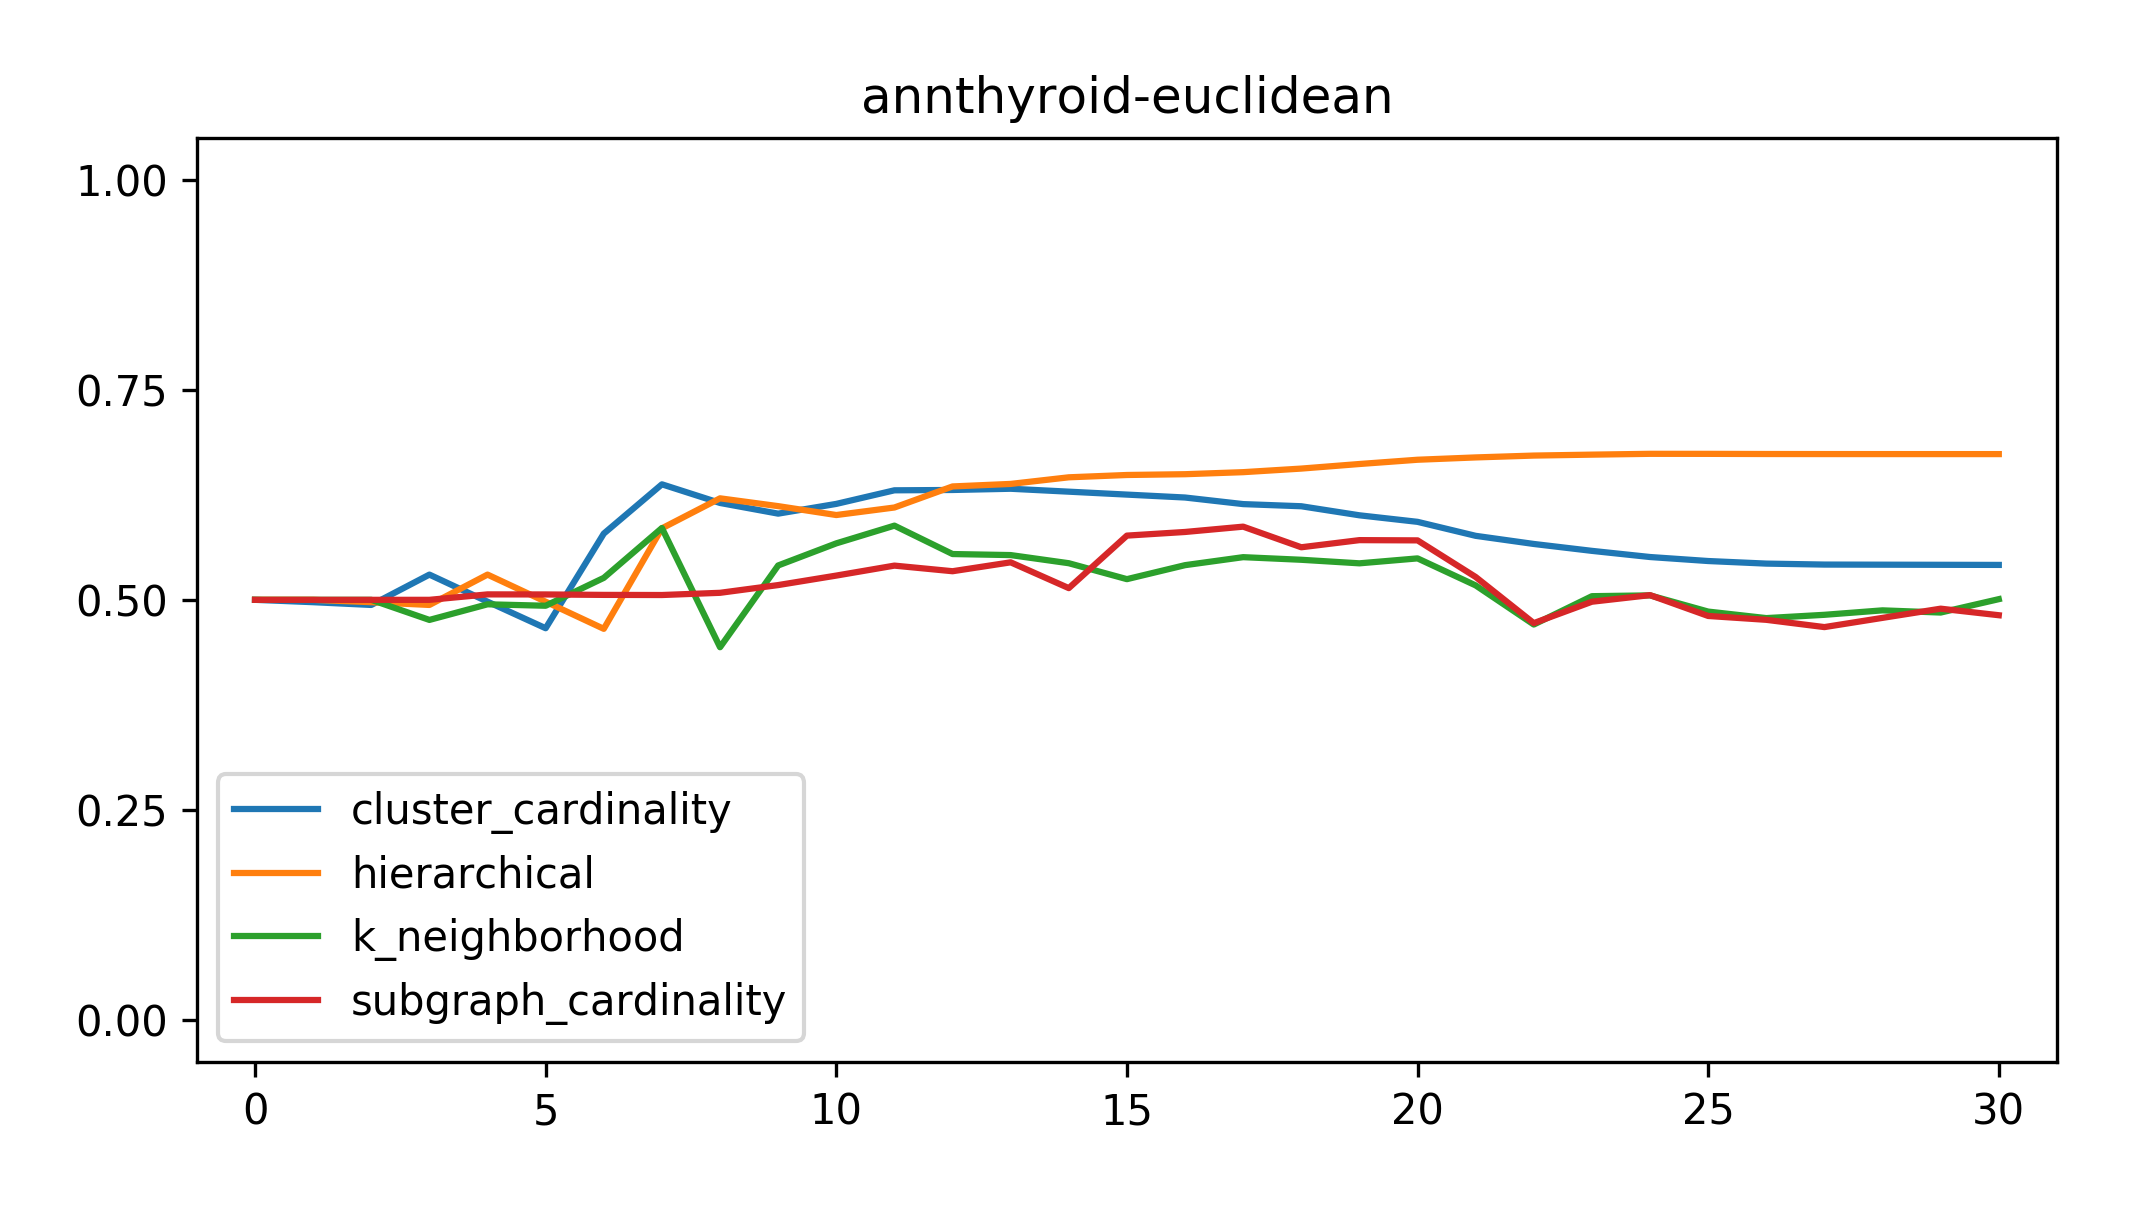
\includegraphics[width=2.2in]{kdd/static/auc_vs_depth/annthyroid-euclidean.png}
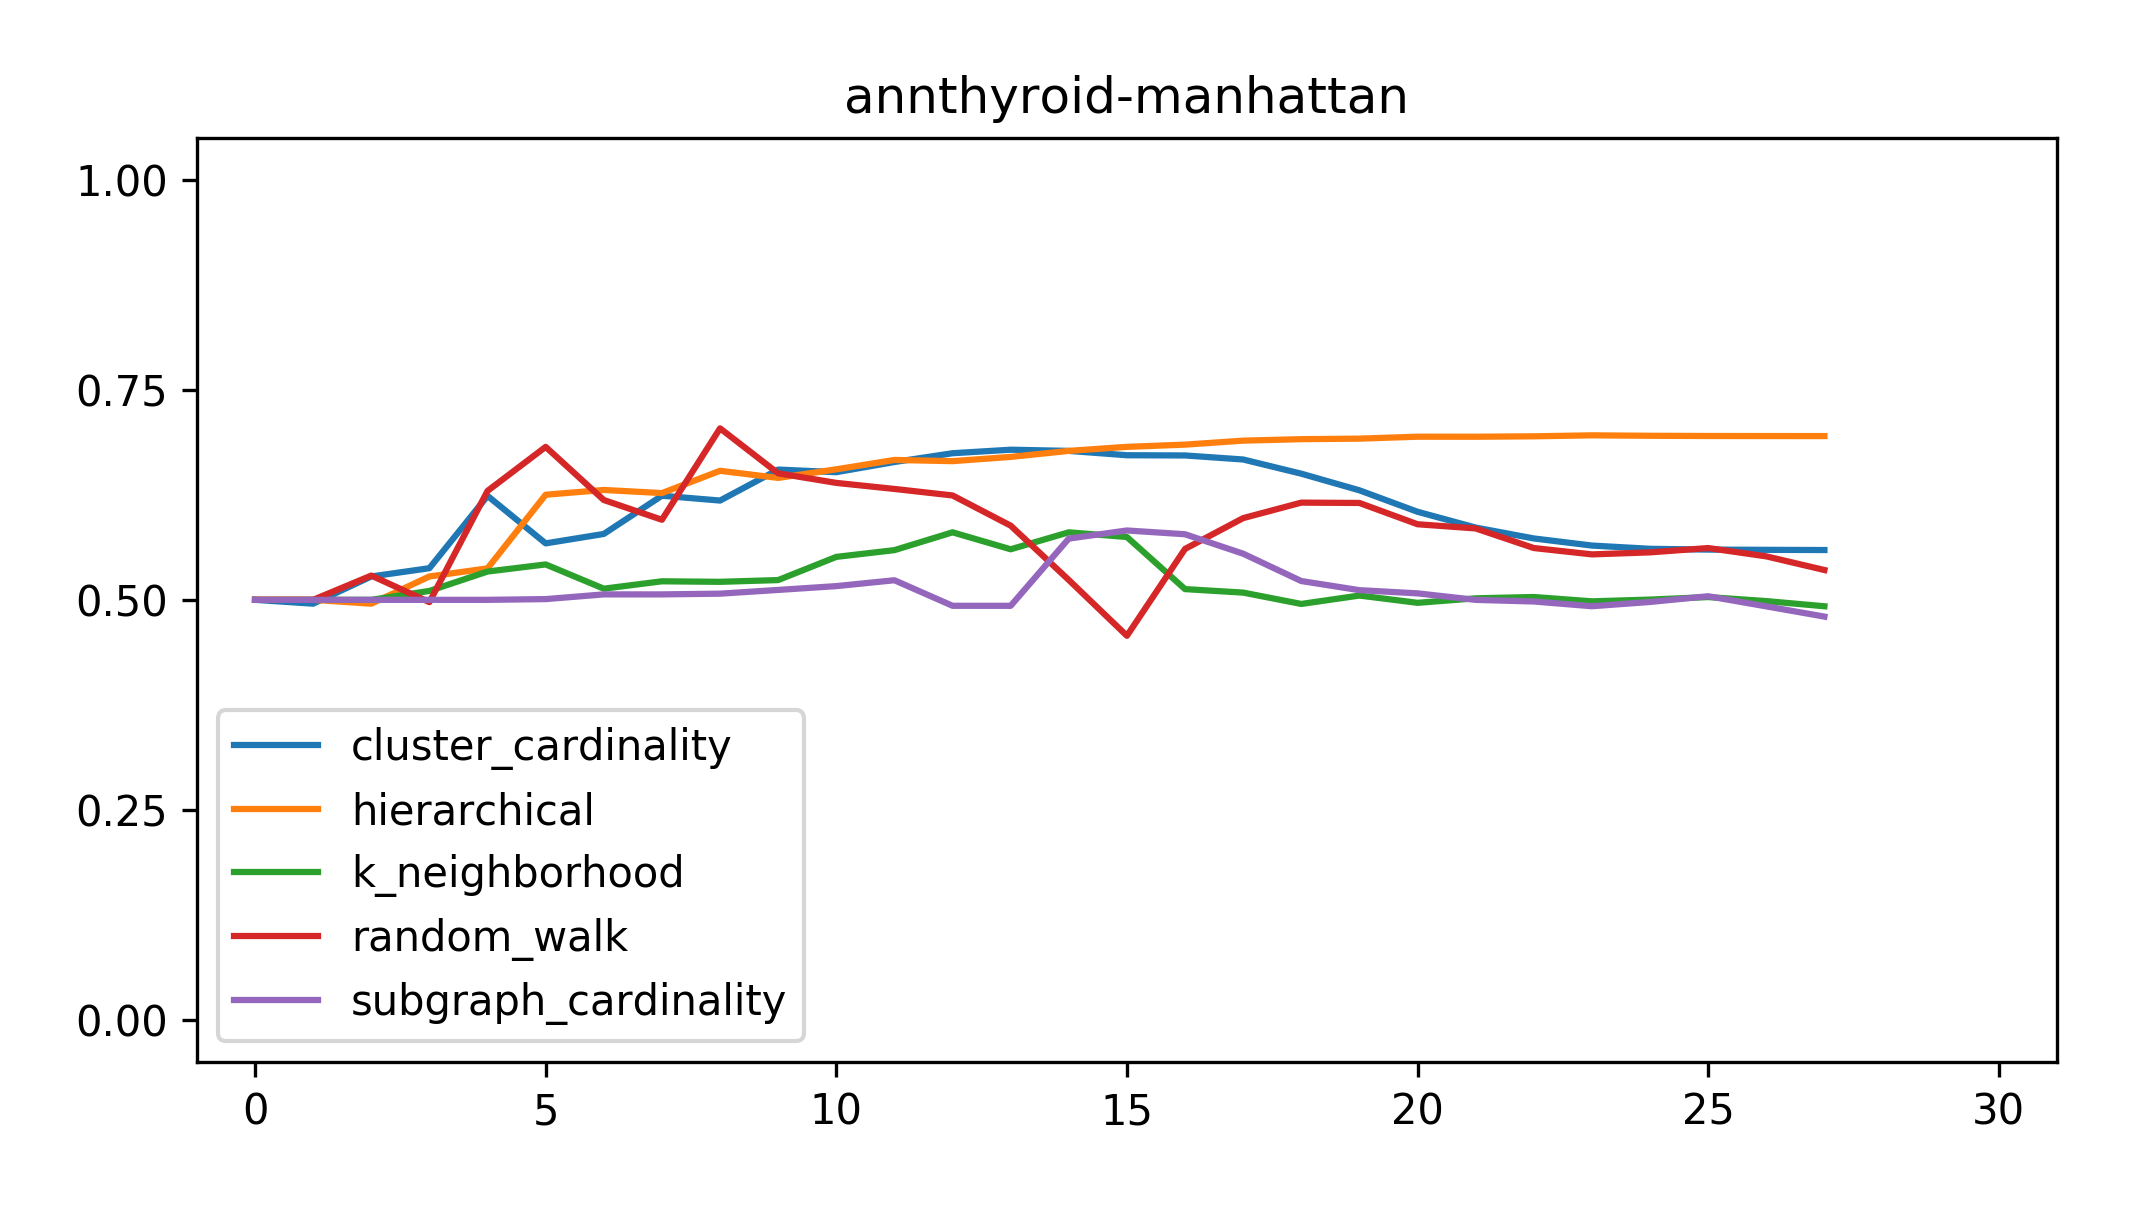
\includegraphics[width=2.2in]{kdd/static/auc_vs_depth/annthyroid-manhattan.png}

% Arrhythmia
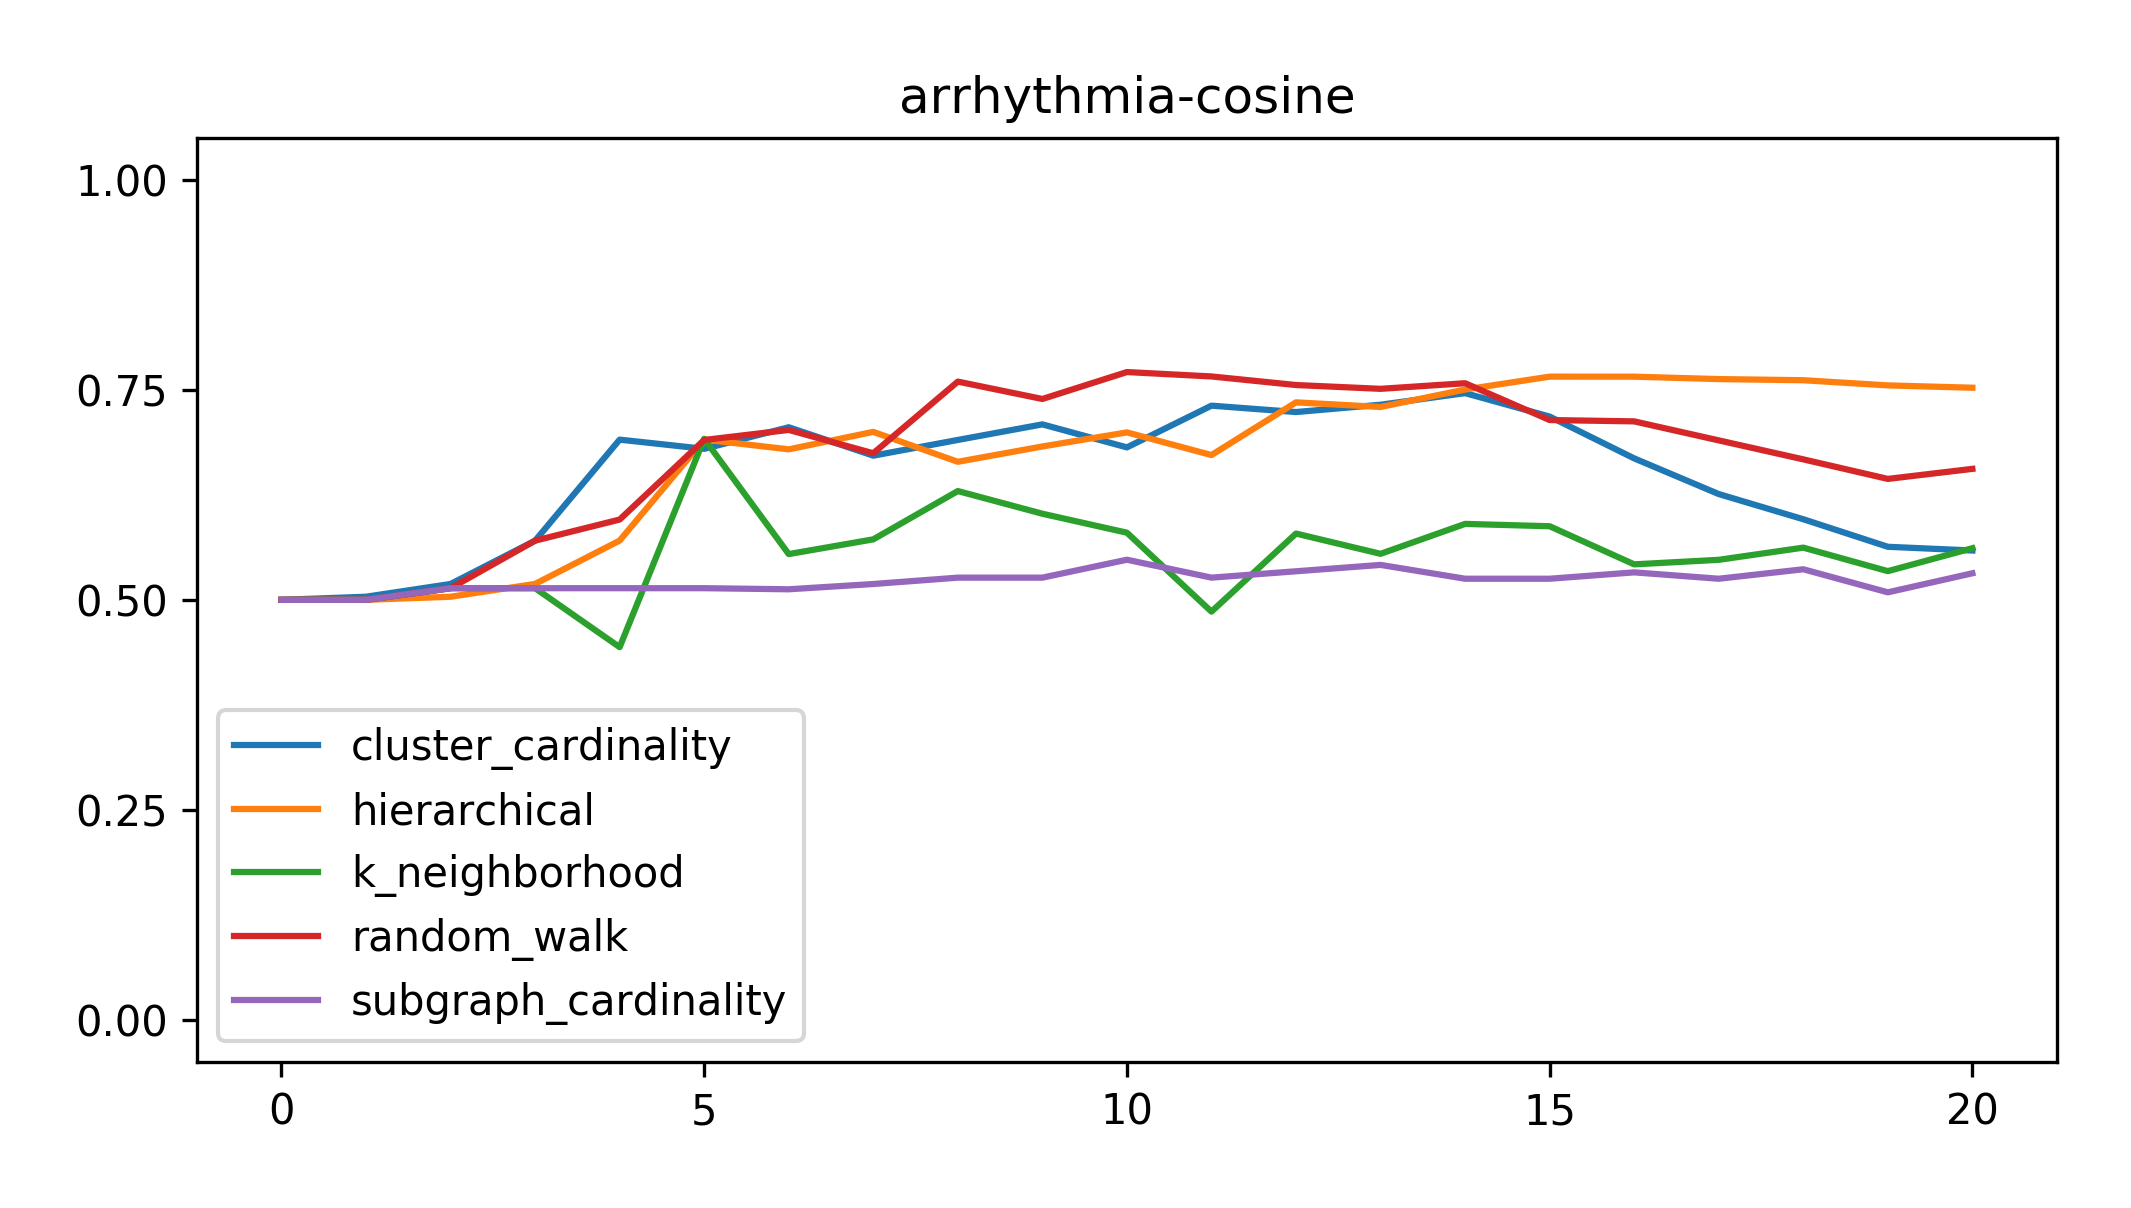
\includegraphics[width=2.2in]{kdd/static/auc_vs_depth/arrhythmia-cosine.png}
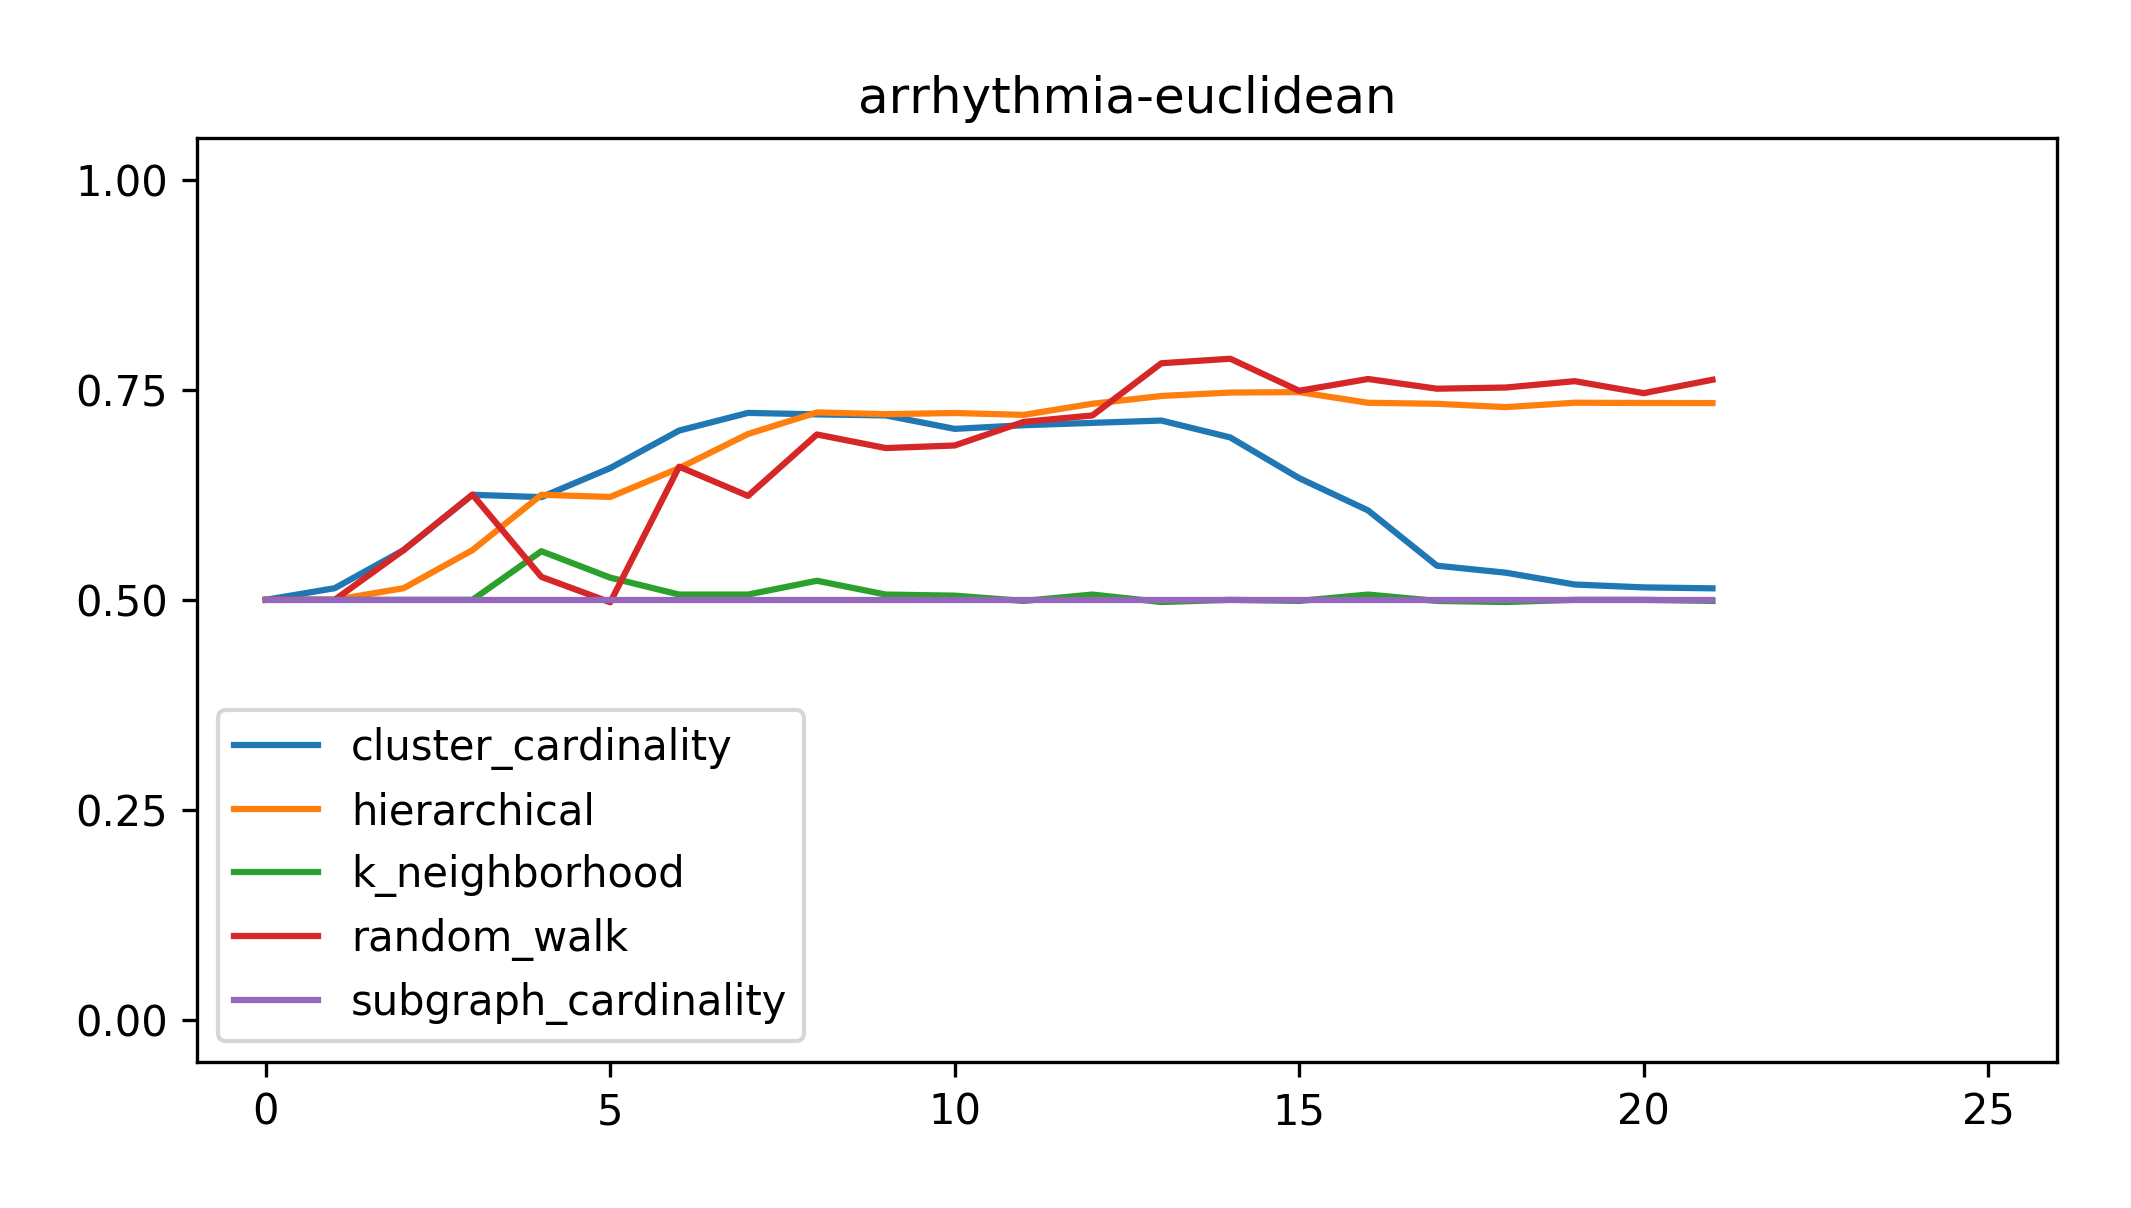
\includegraphics[width=2.2in]{kdd/static/auc_vs_depth/arrhythmia-euclidean.png}
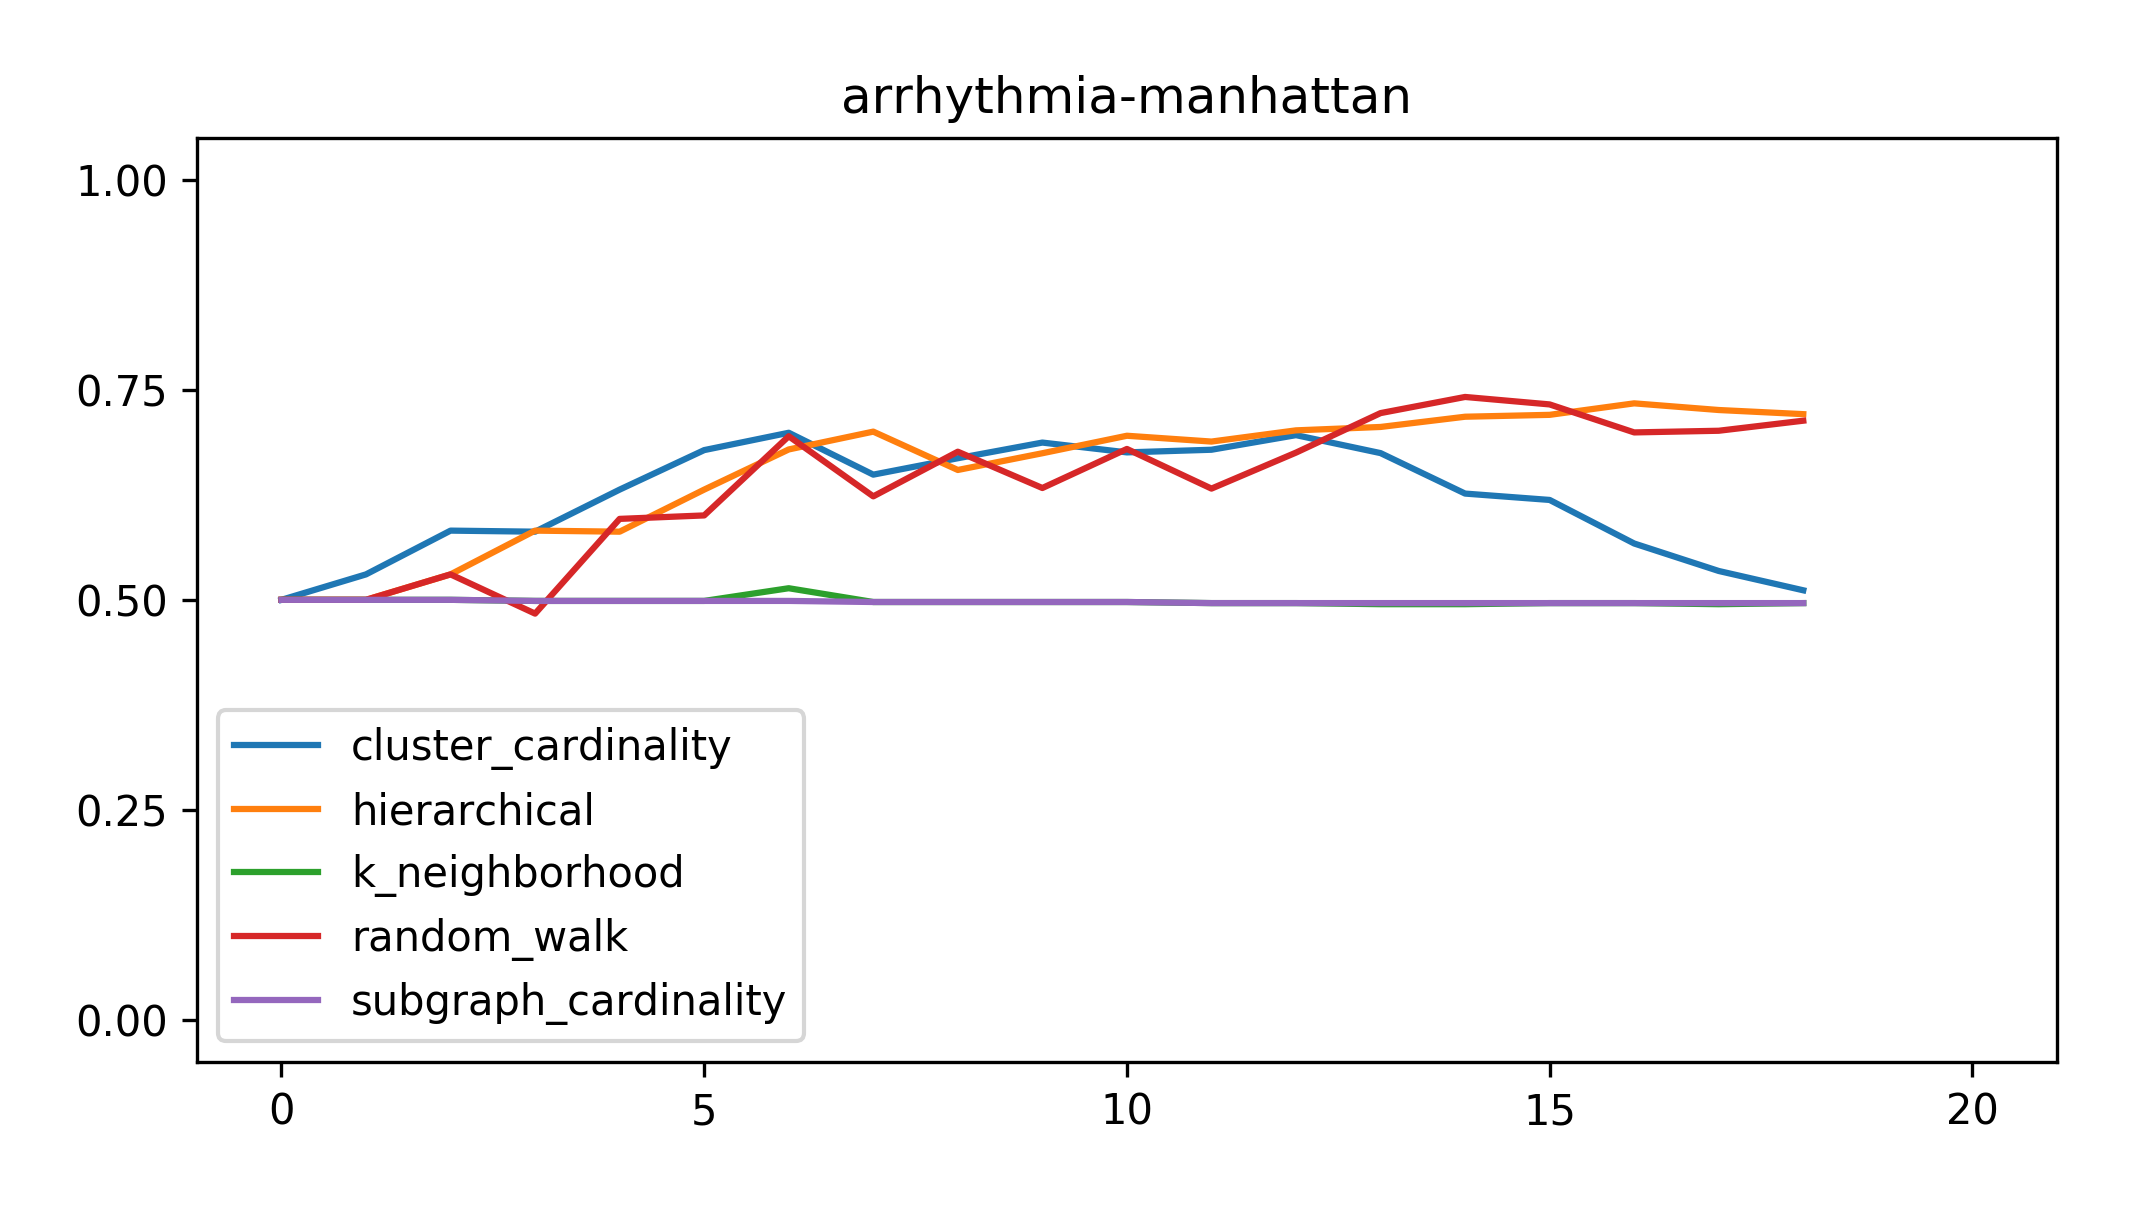
\includegraphics[width=2.2in]{kdd/static/auc_vs_depth/arrhythmia-manhattan.png}

% BreastW
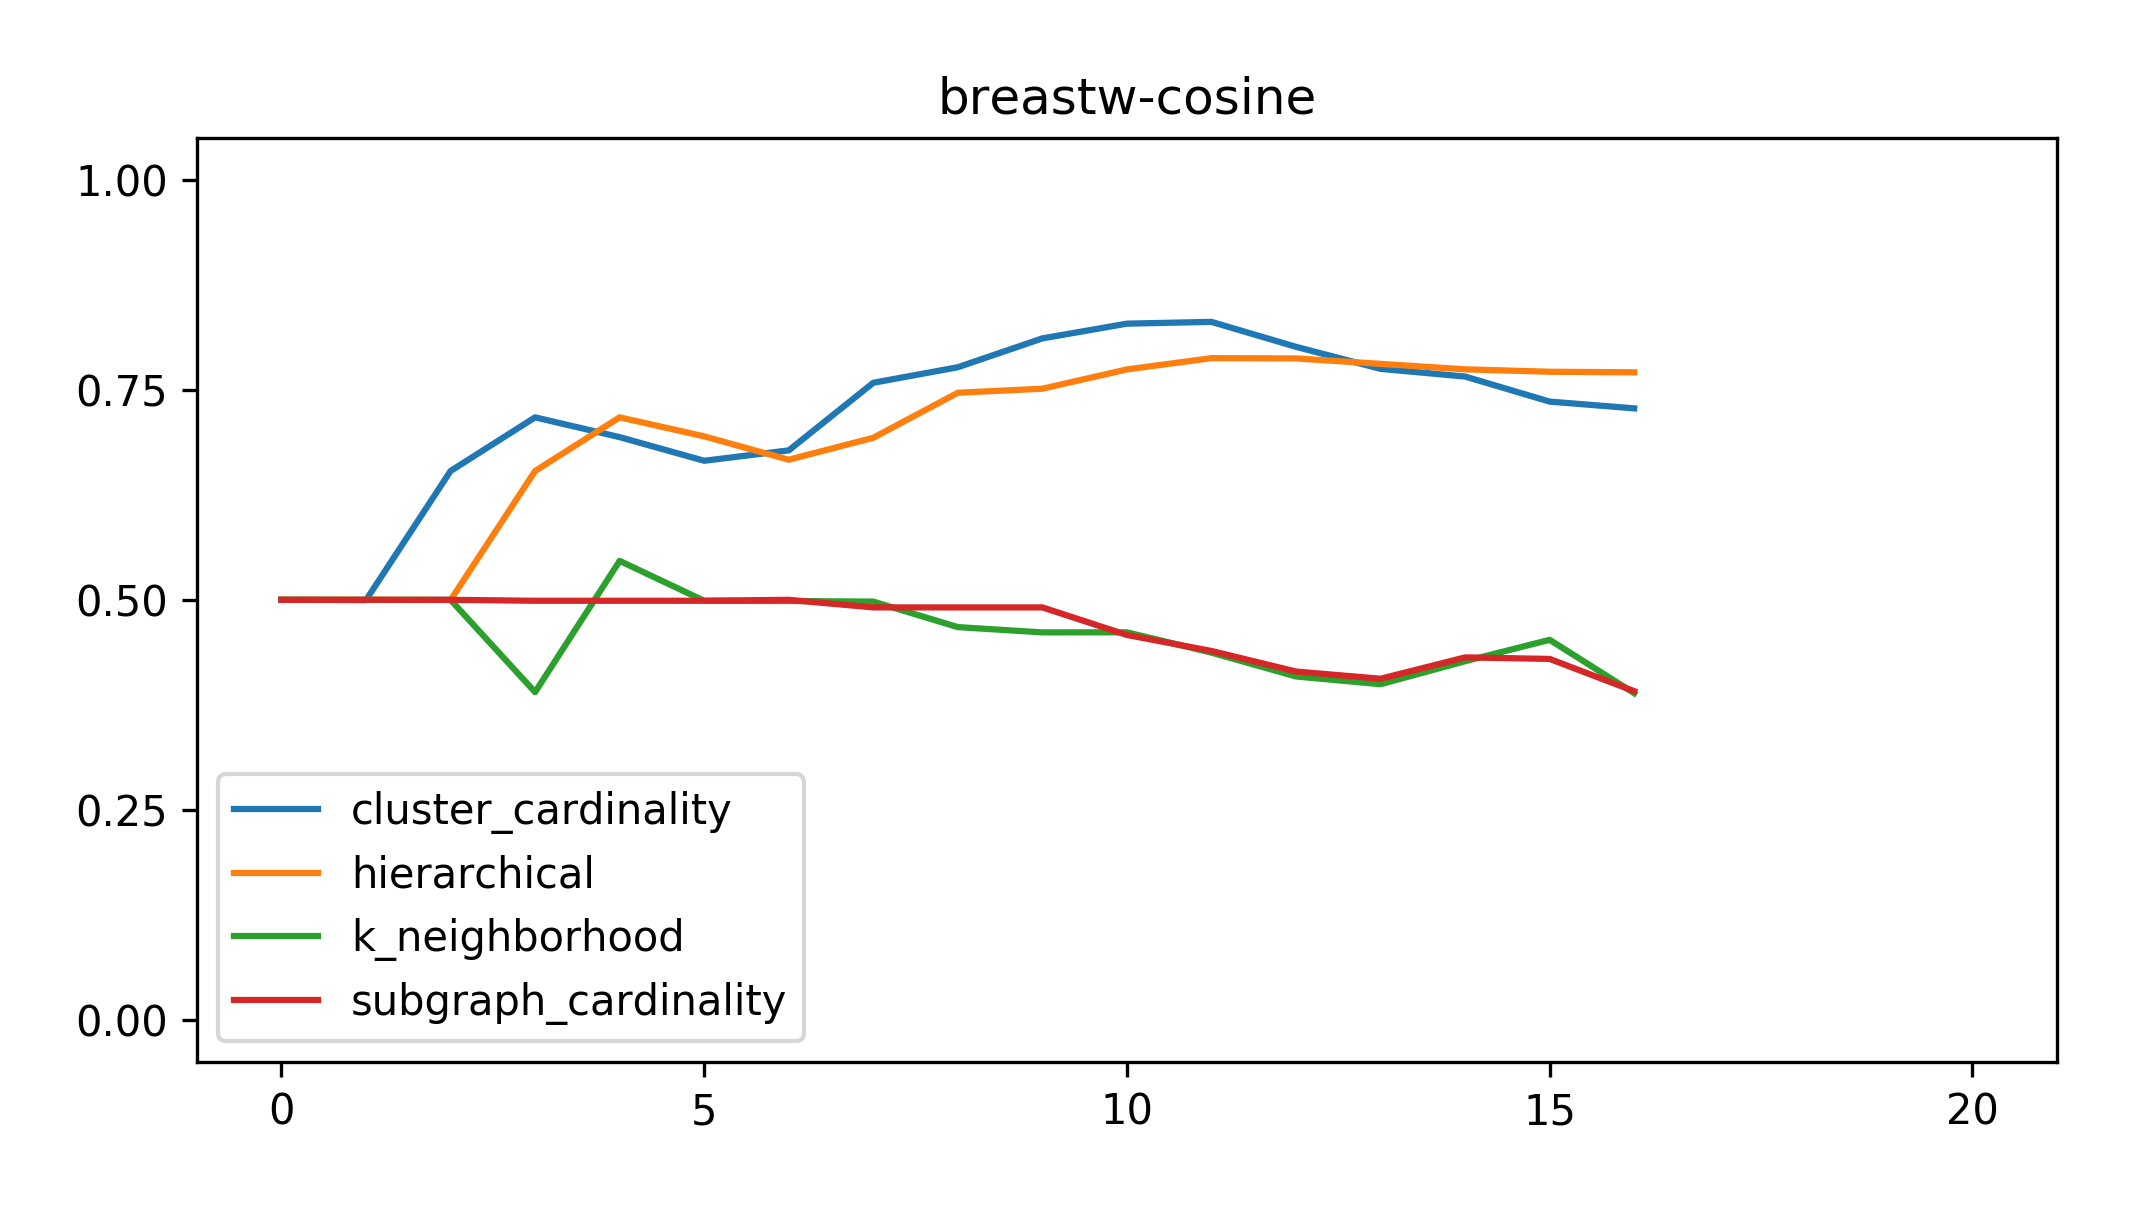
\includegraphics[width=2.2in]{kdd/static/auc_vs_depth/breastw-cosine.png}
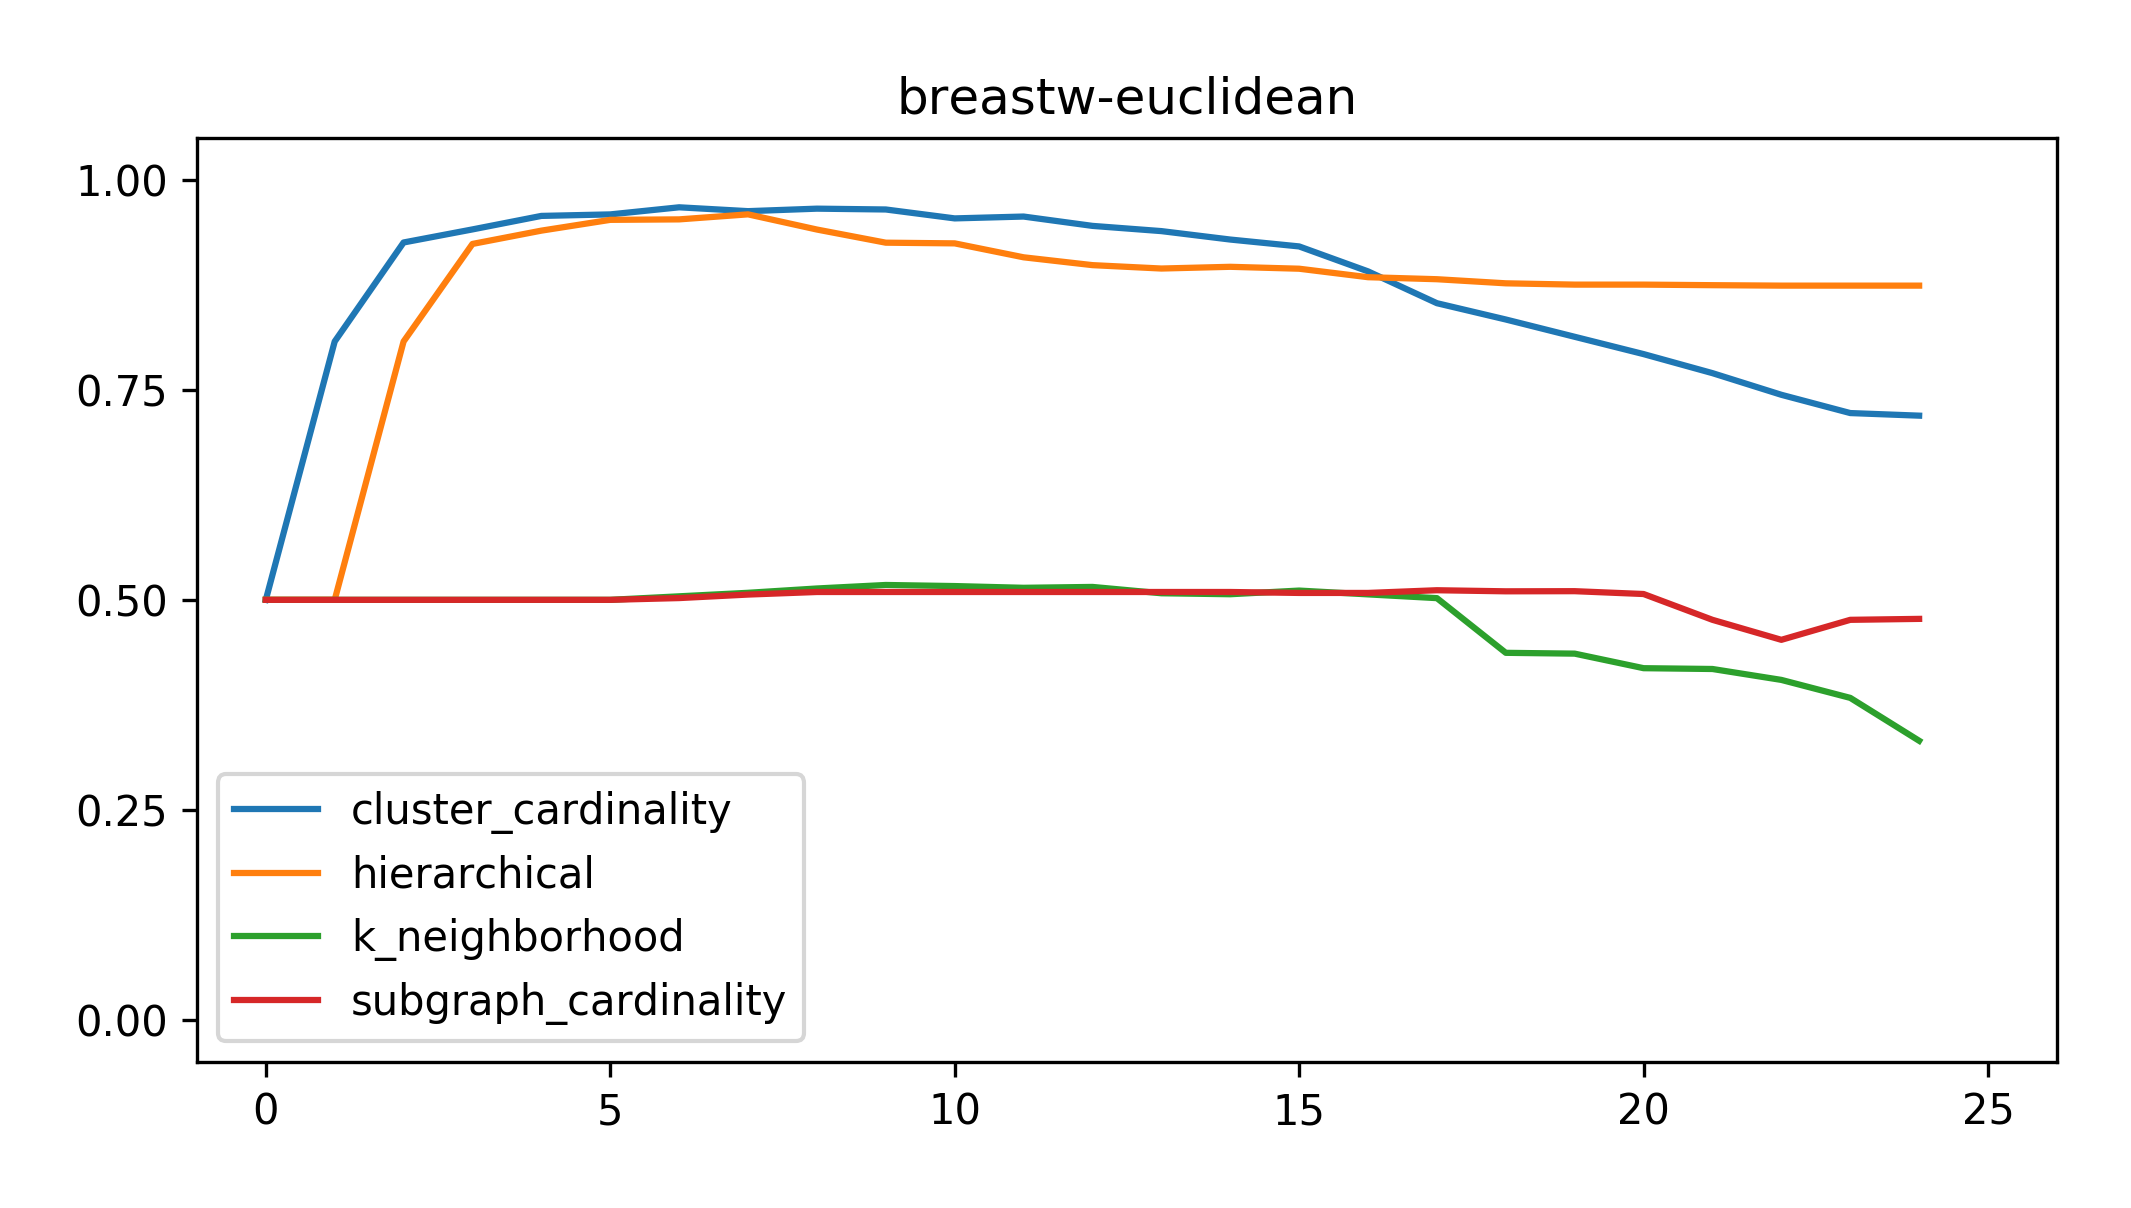
\includegraphics[width=2.2in]{kdd/static/auc_vs_depth/breastw-euclidean.png}
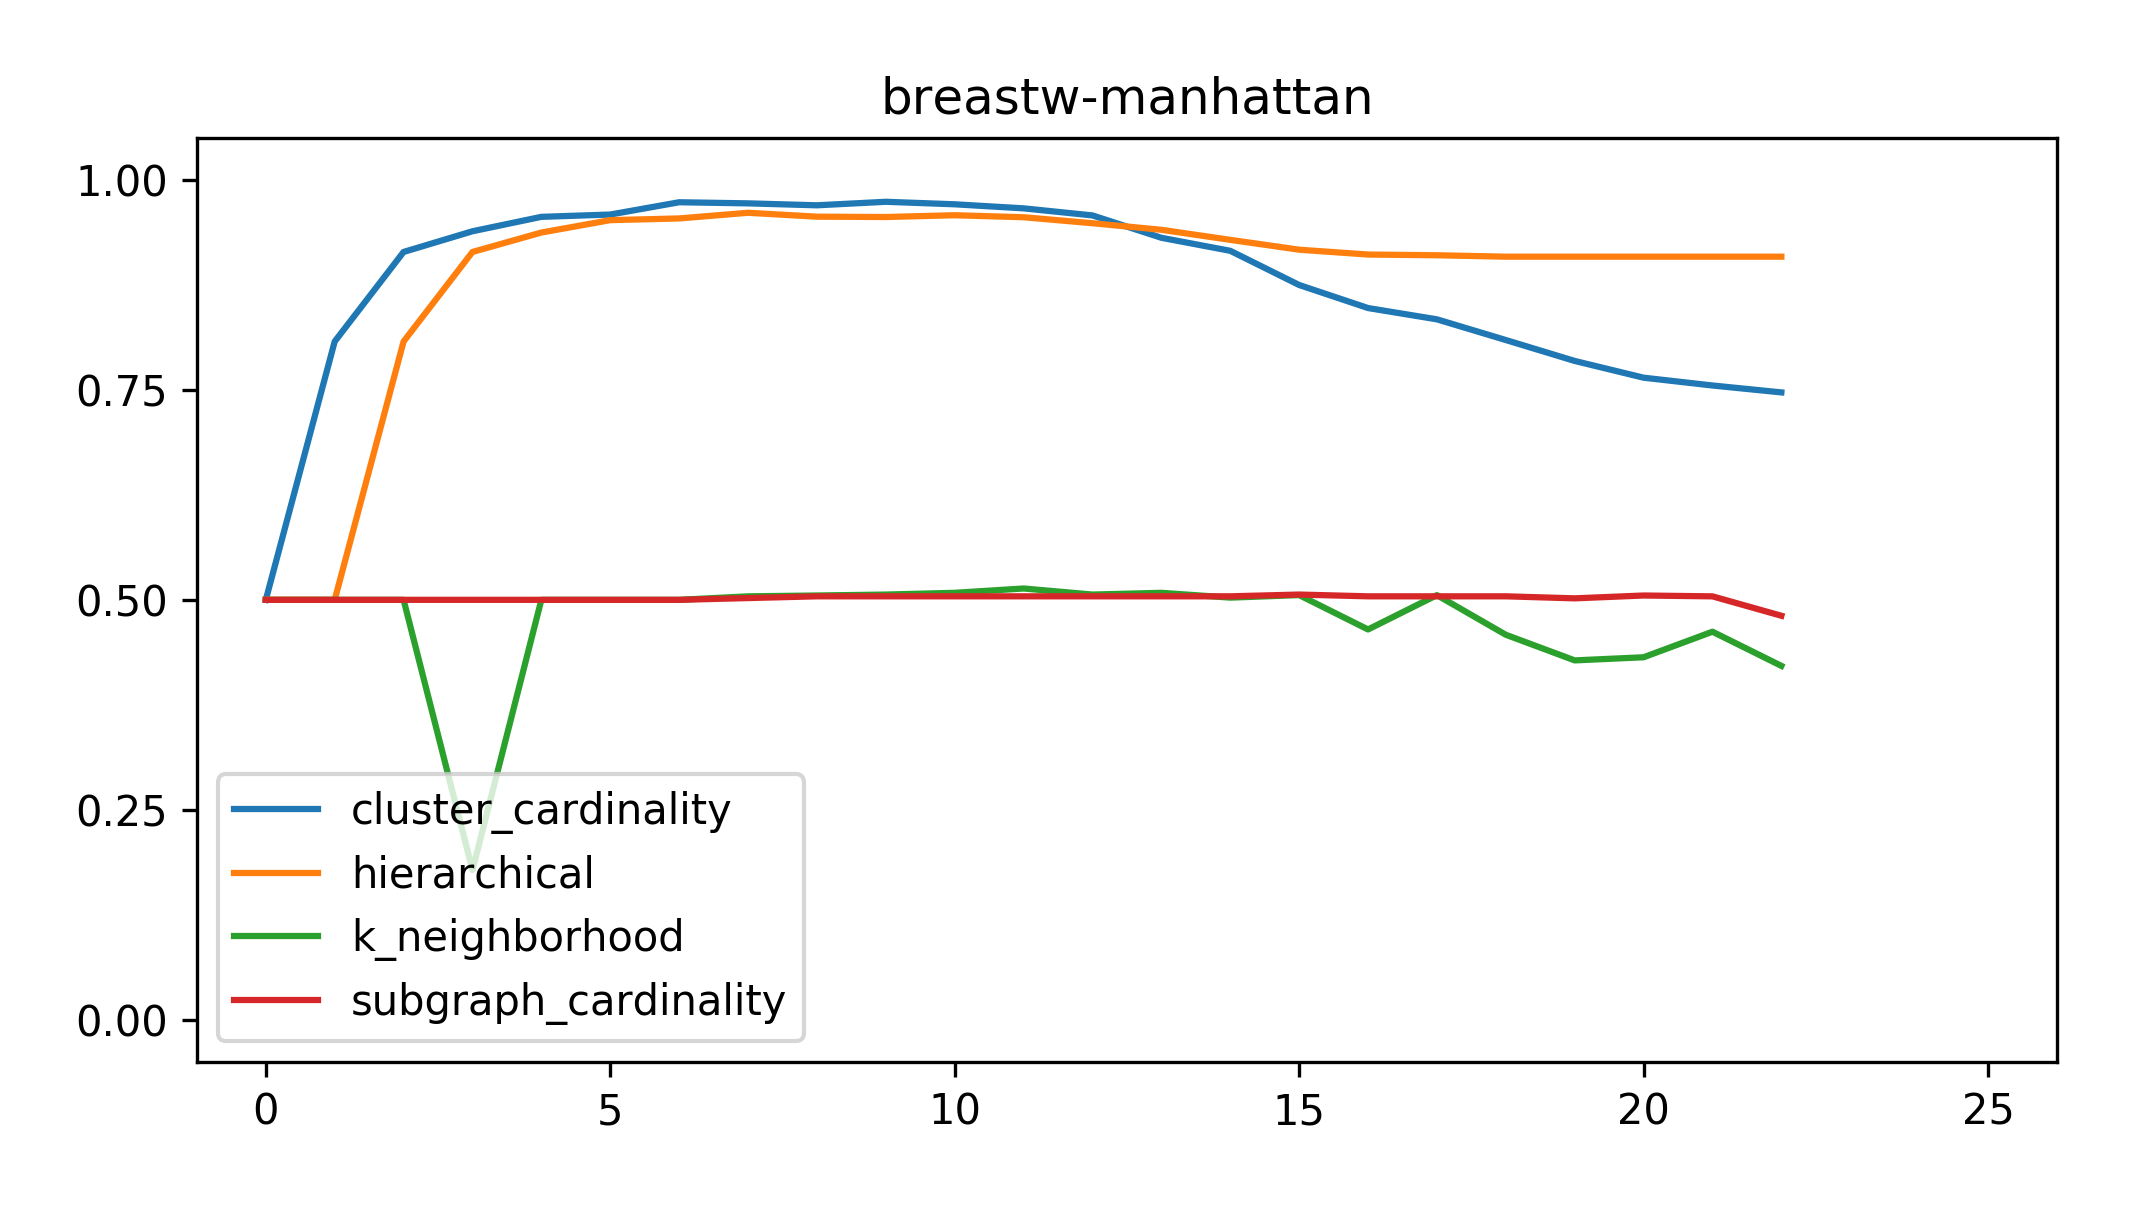
\includegraphics[width=2.2in]{kdd/static/auc_vs_depth/breastw-manhattan.png}

% Cardio
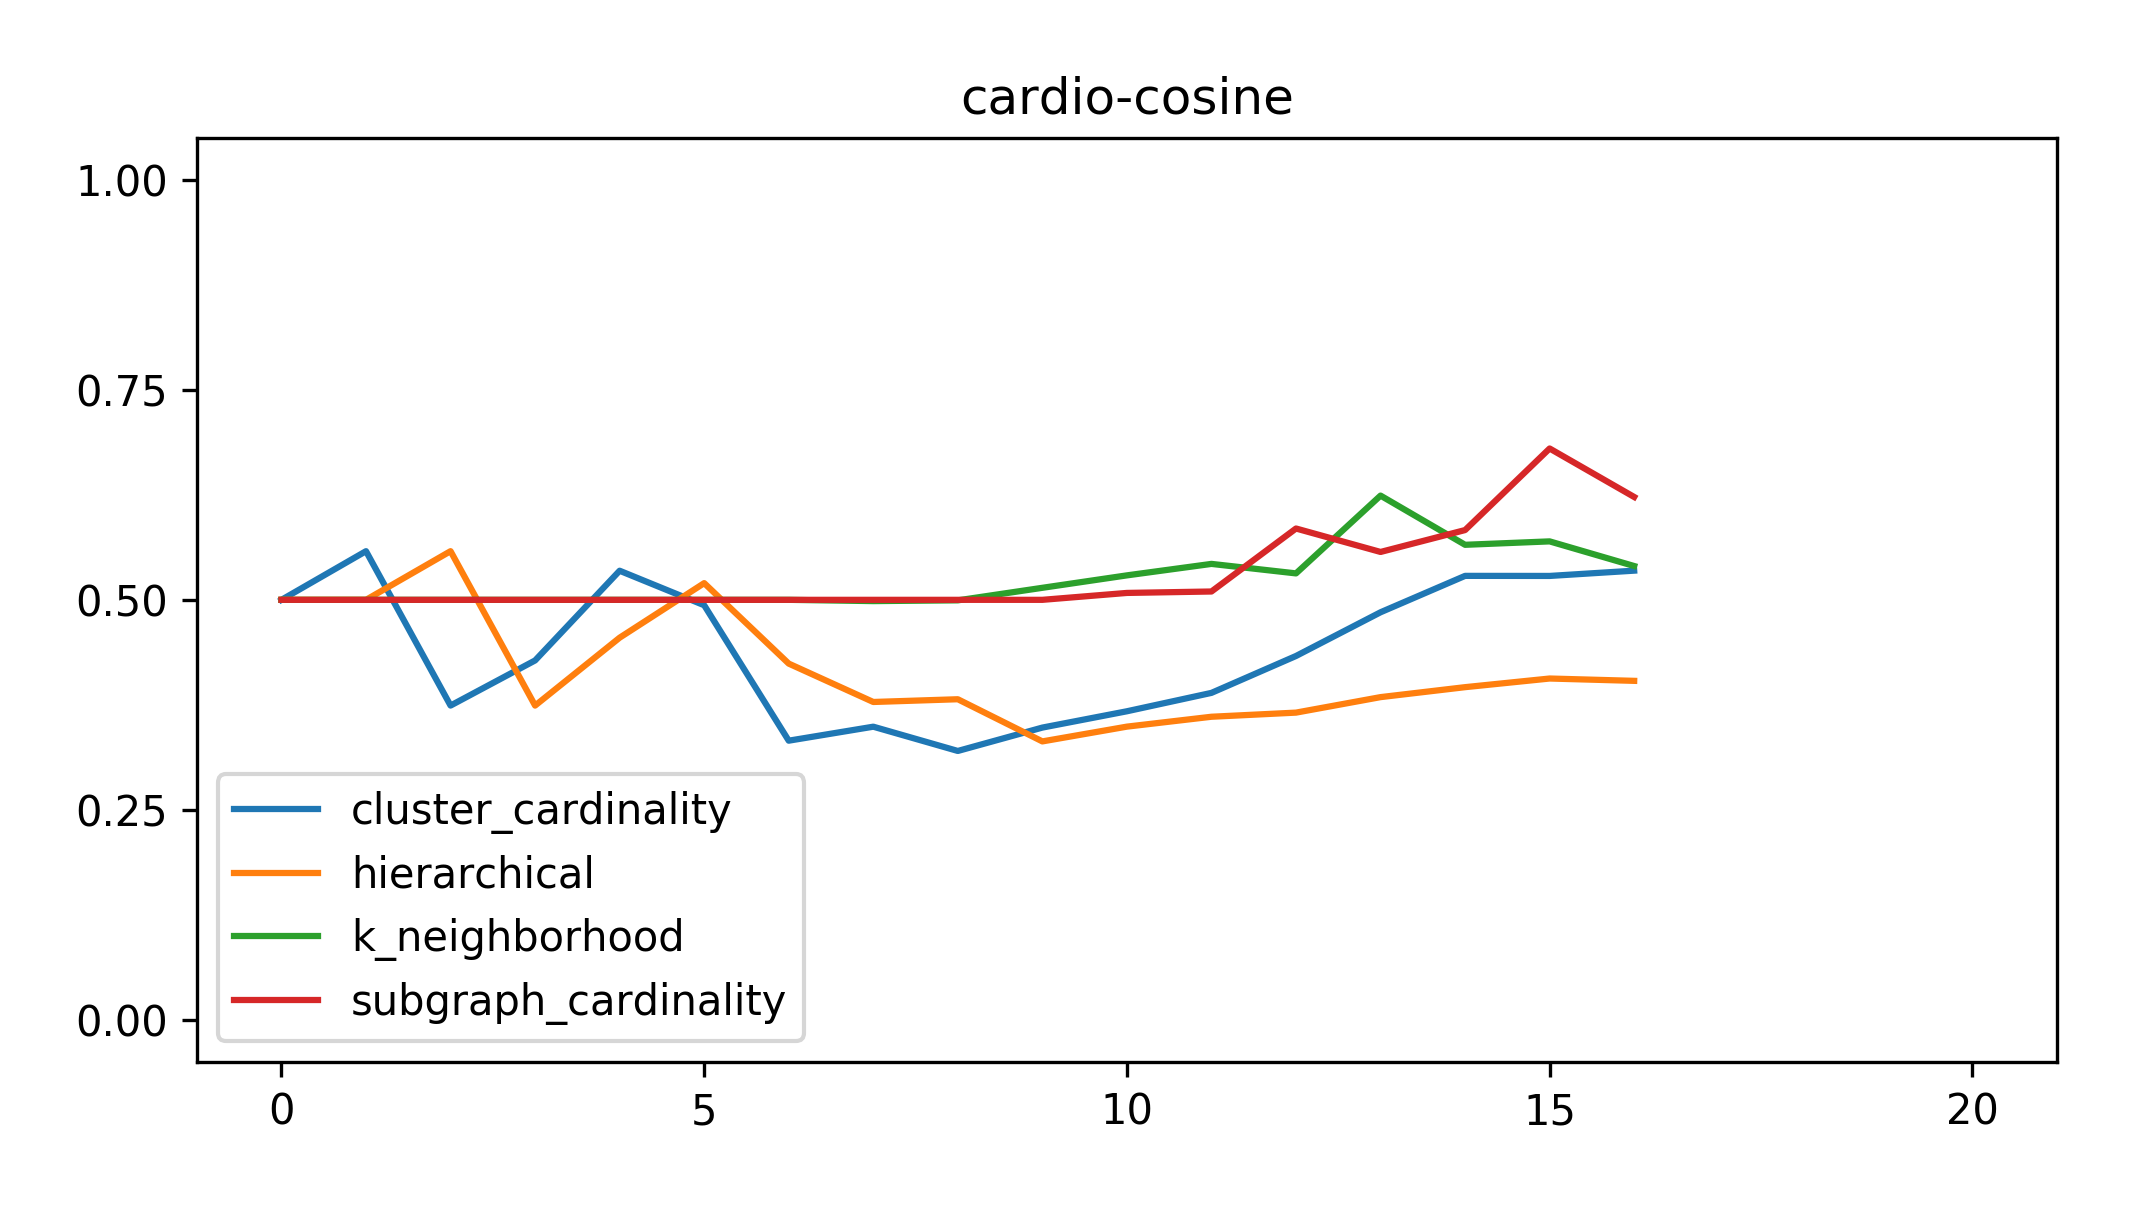
\includegraphics[width=2.2in]{kdd/static/auc_vs_depth/cardio-cosine.png}
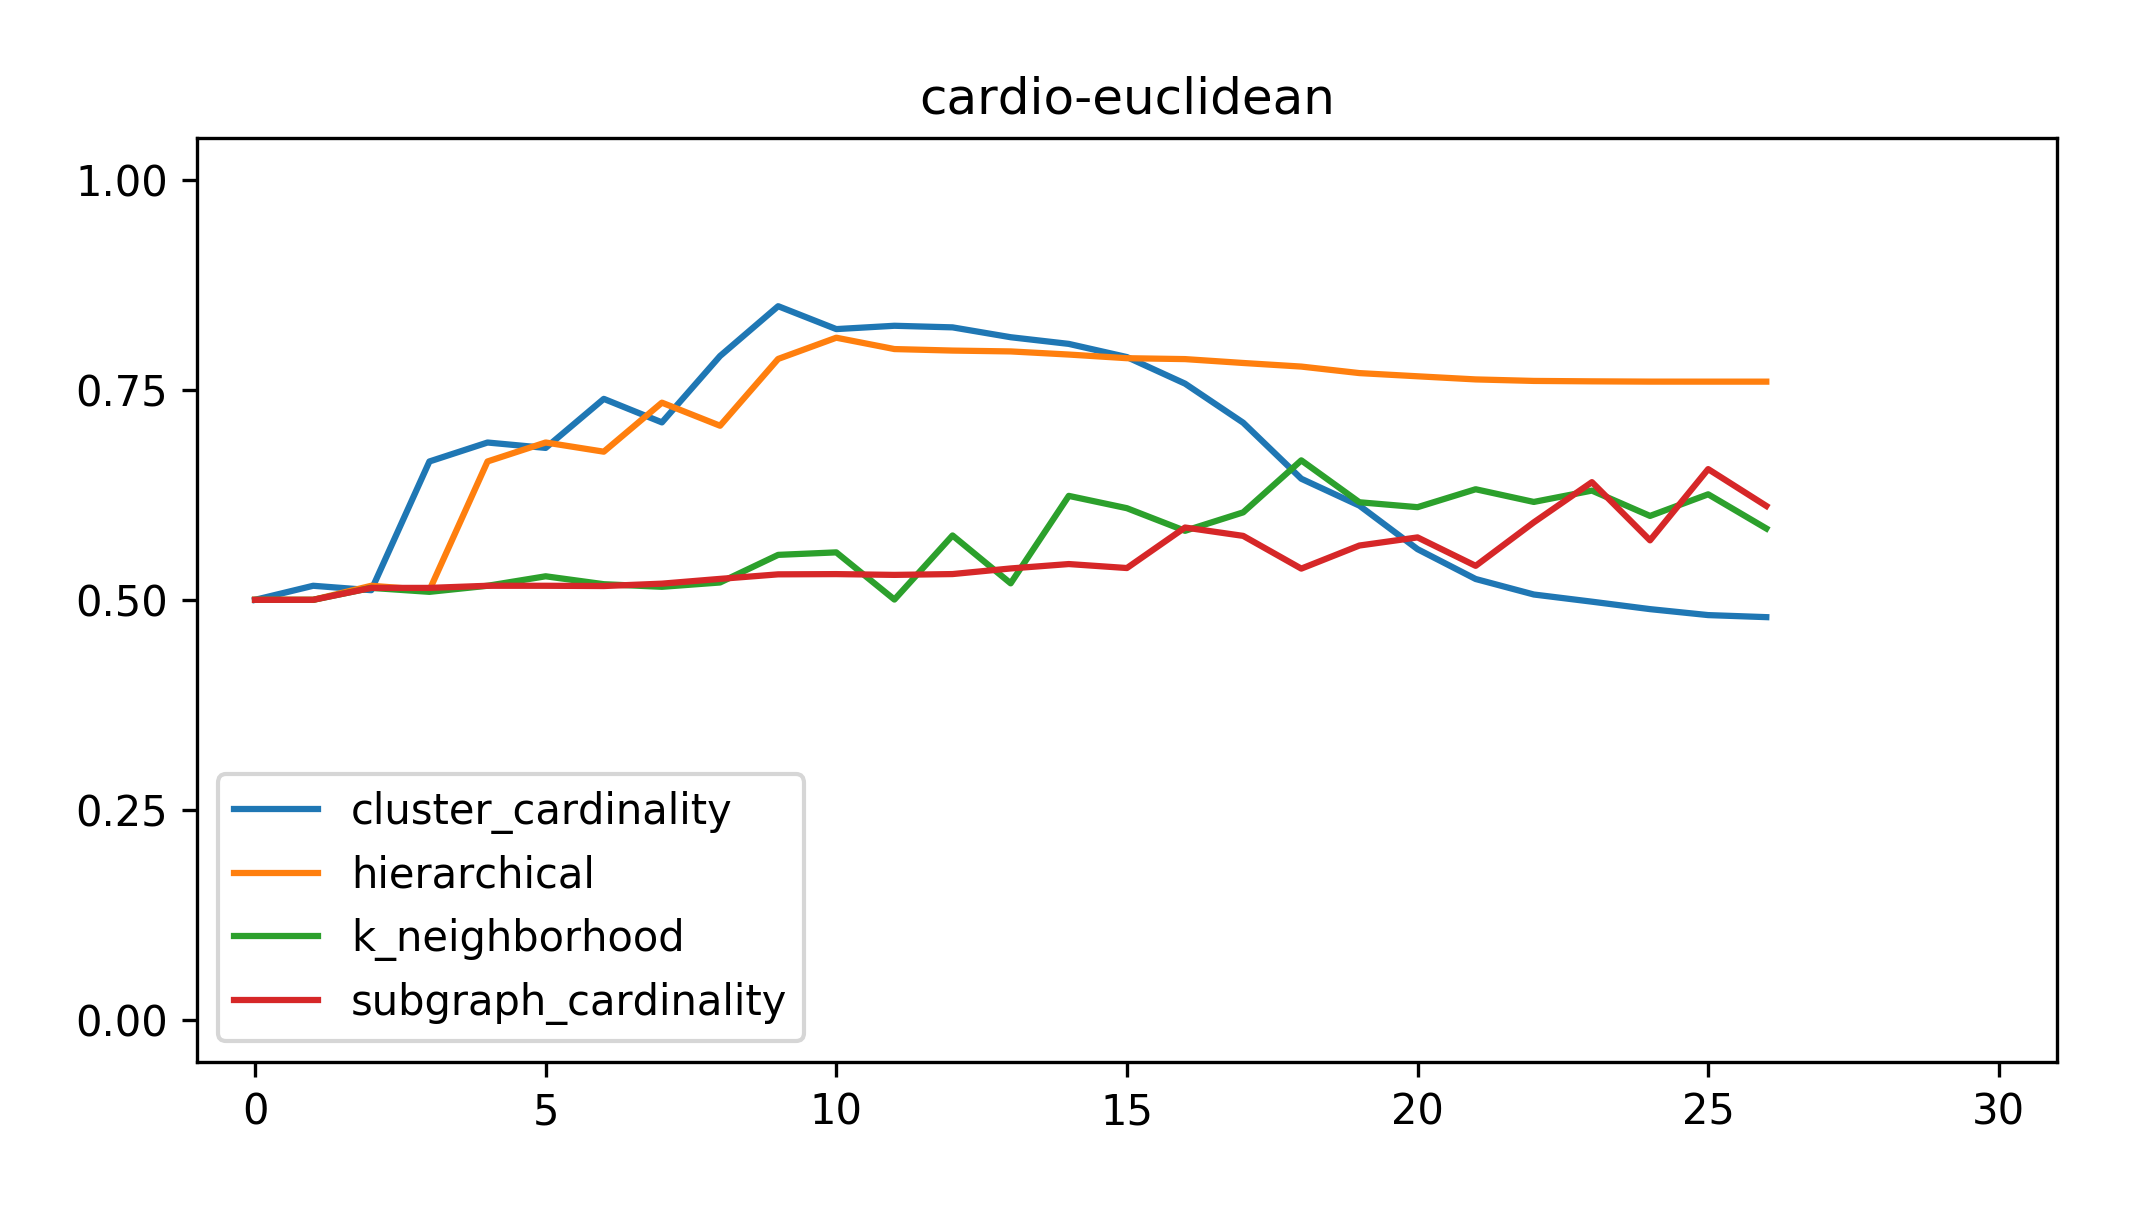
\includegraphics[width=2.2in]{kdd/static/auc_vs_depth/cardio-euclidean.png}
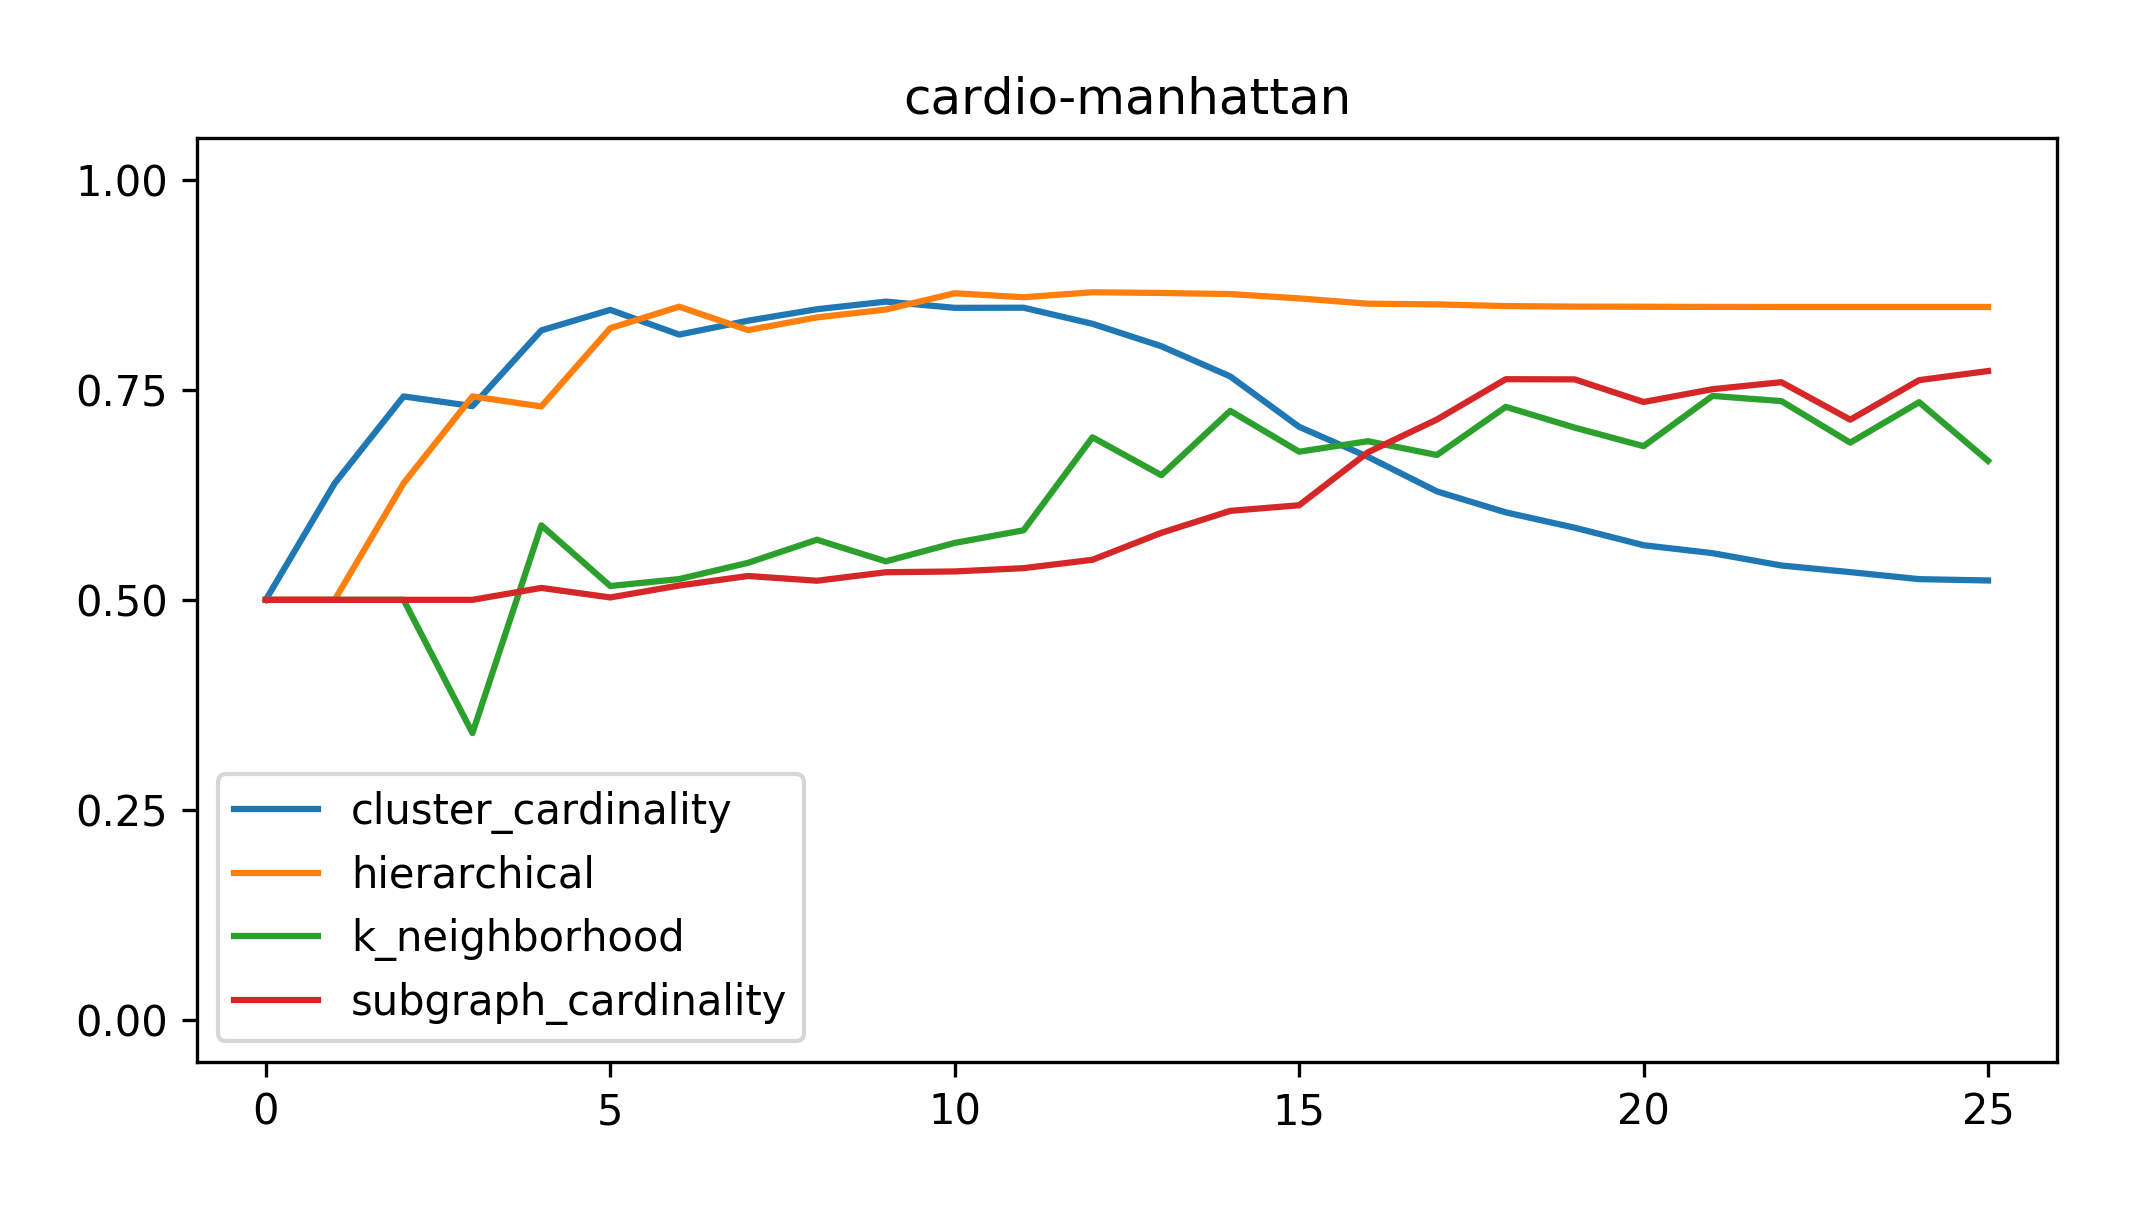
\includegraphics[width=2.2in]{kdd/static/auc_vs_depth/cardio-manhattan.png}

% Glass
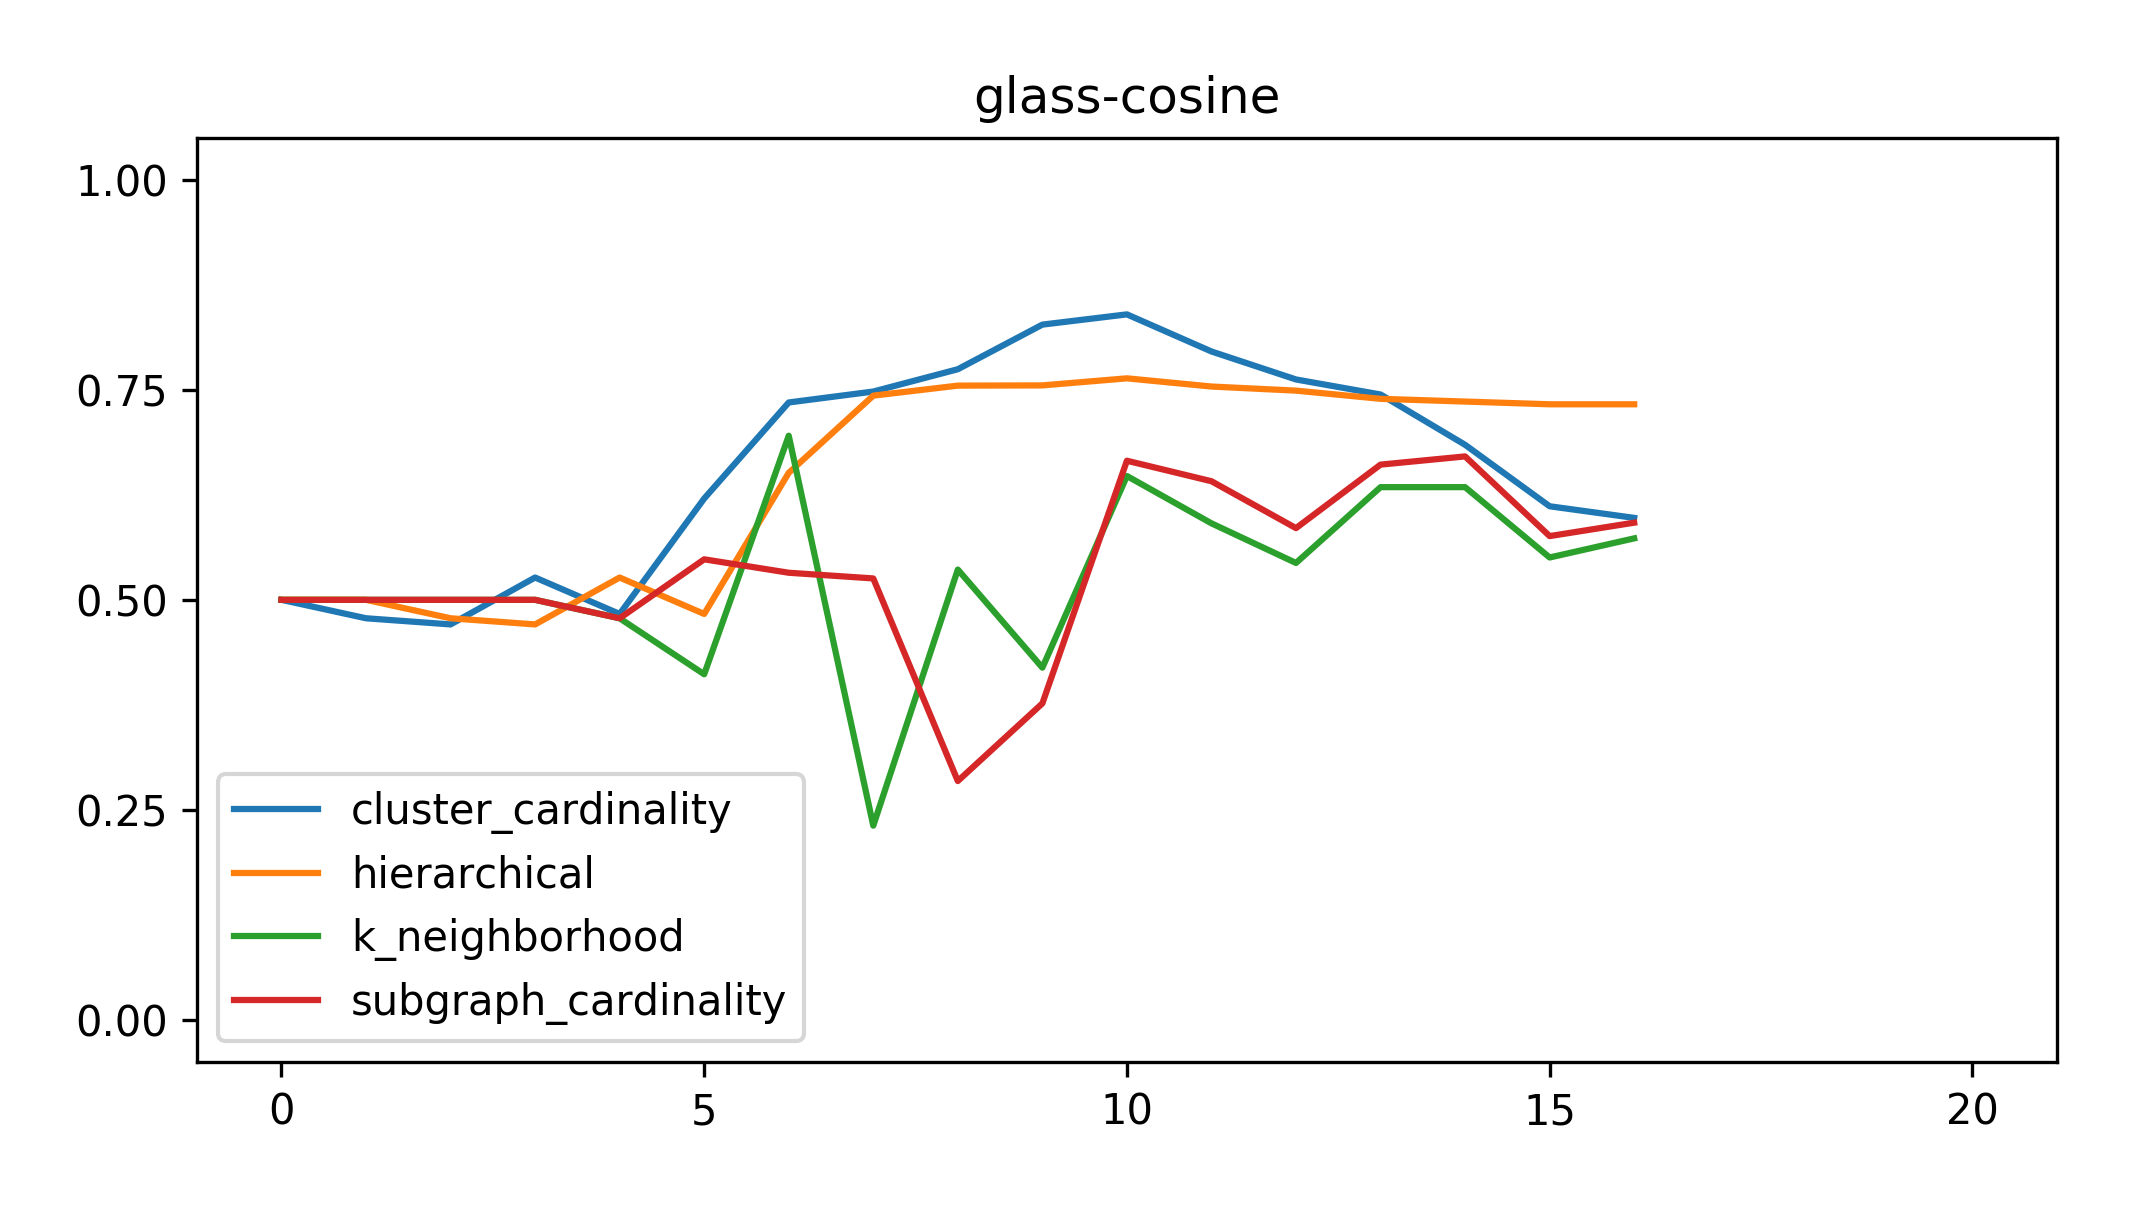
\includegraphics[width=2.2in]{kdd/static/auc_vs_depth/glass-cosine.png}
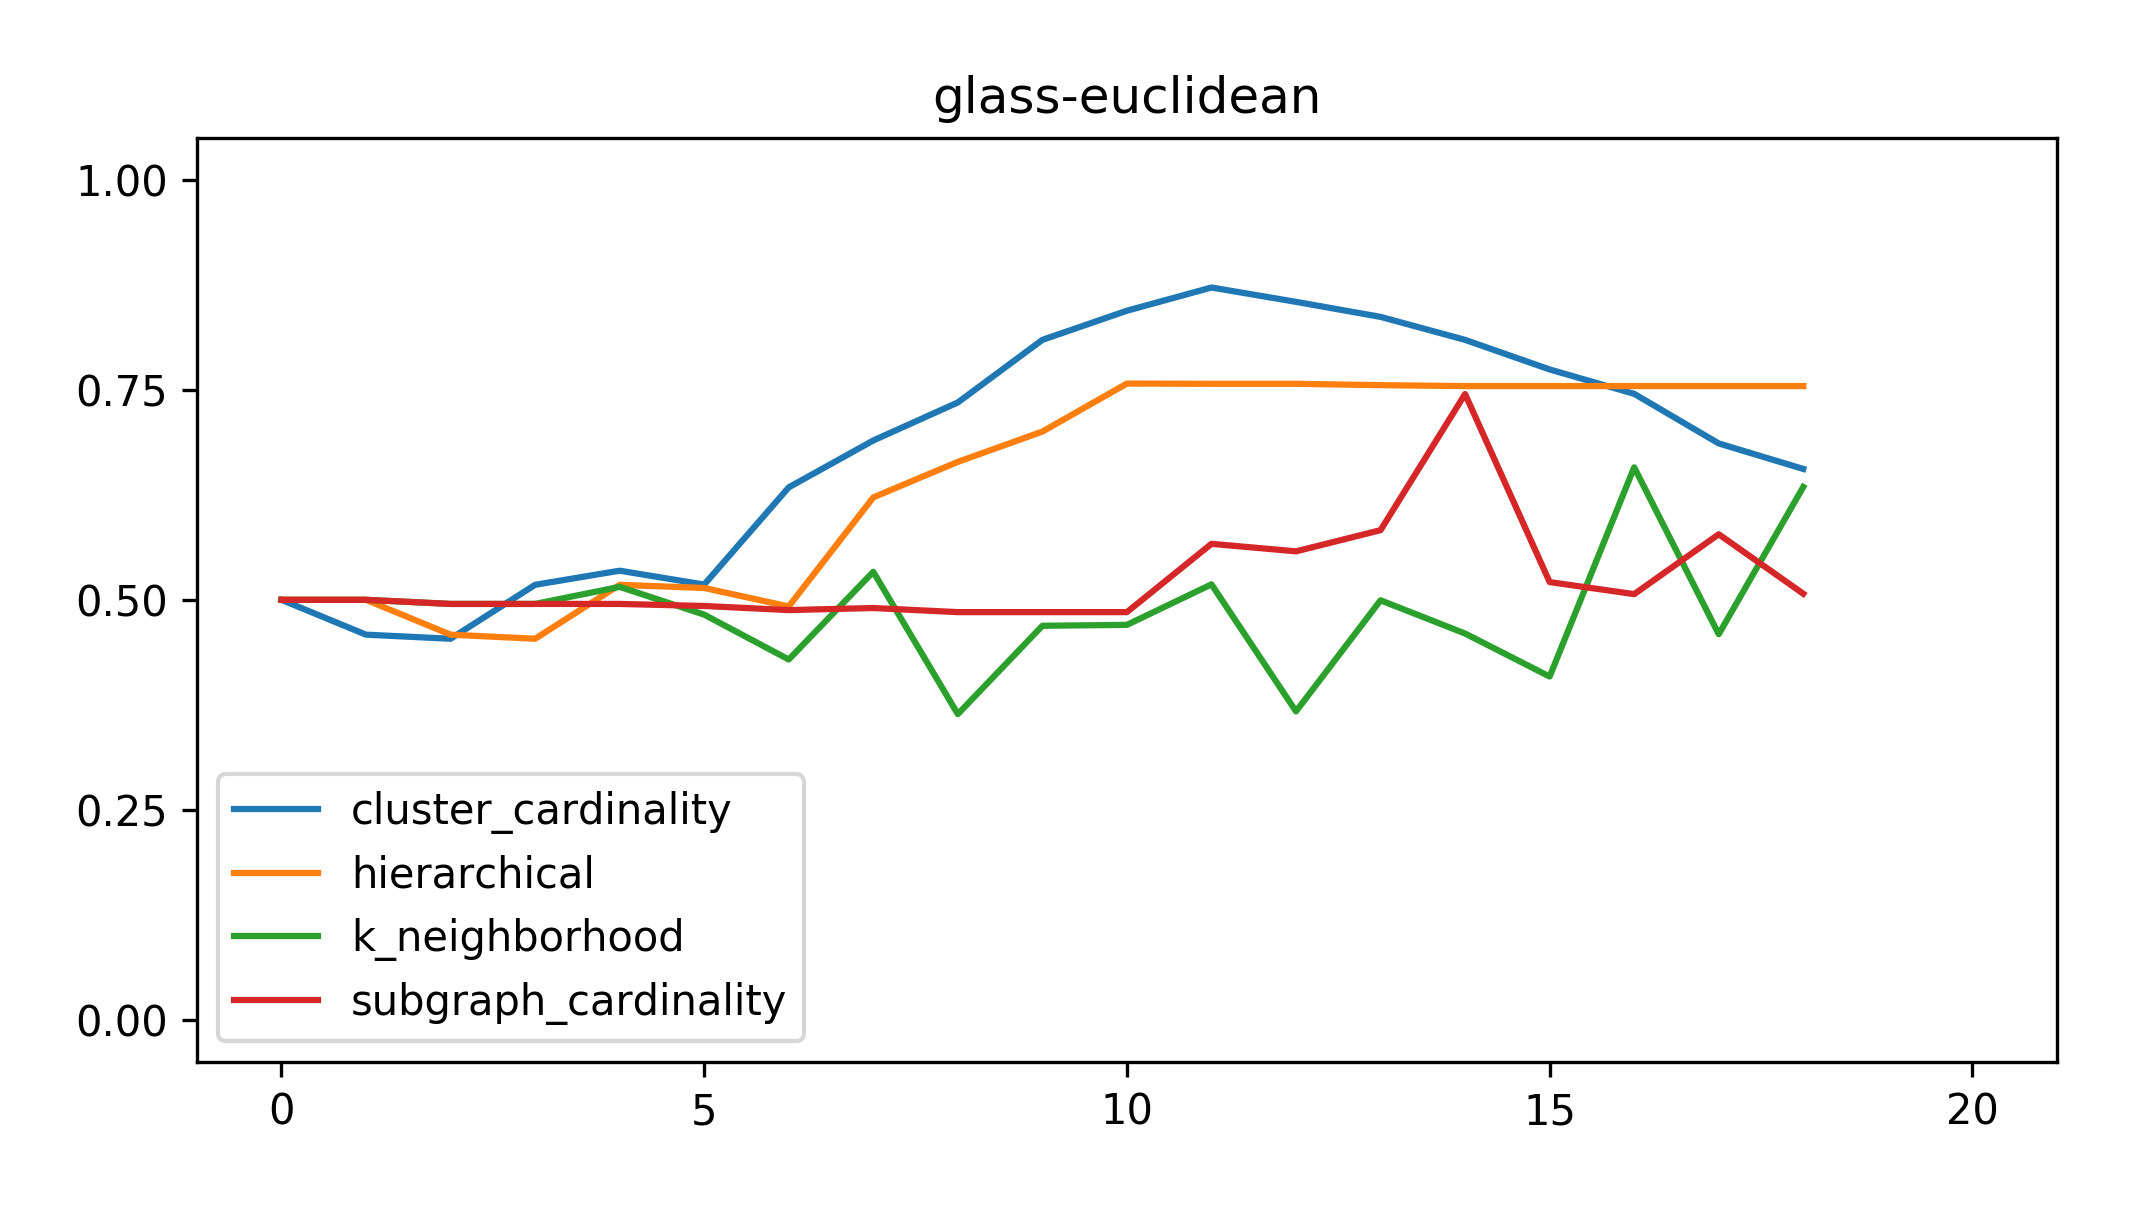
\includegraphics[width=2.2in]{kdd/static/auc_vs_depth/glass-euclidean.png}
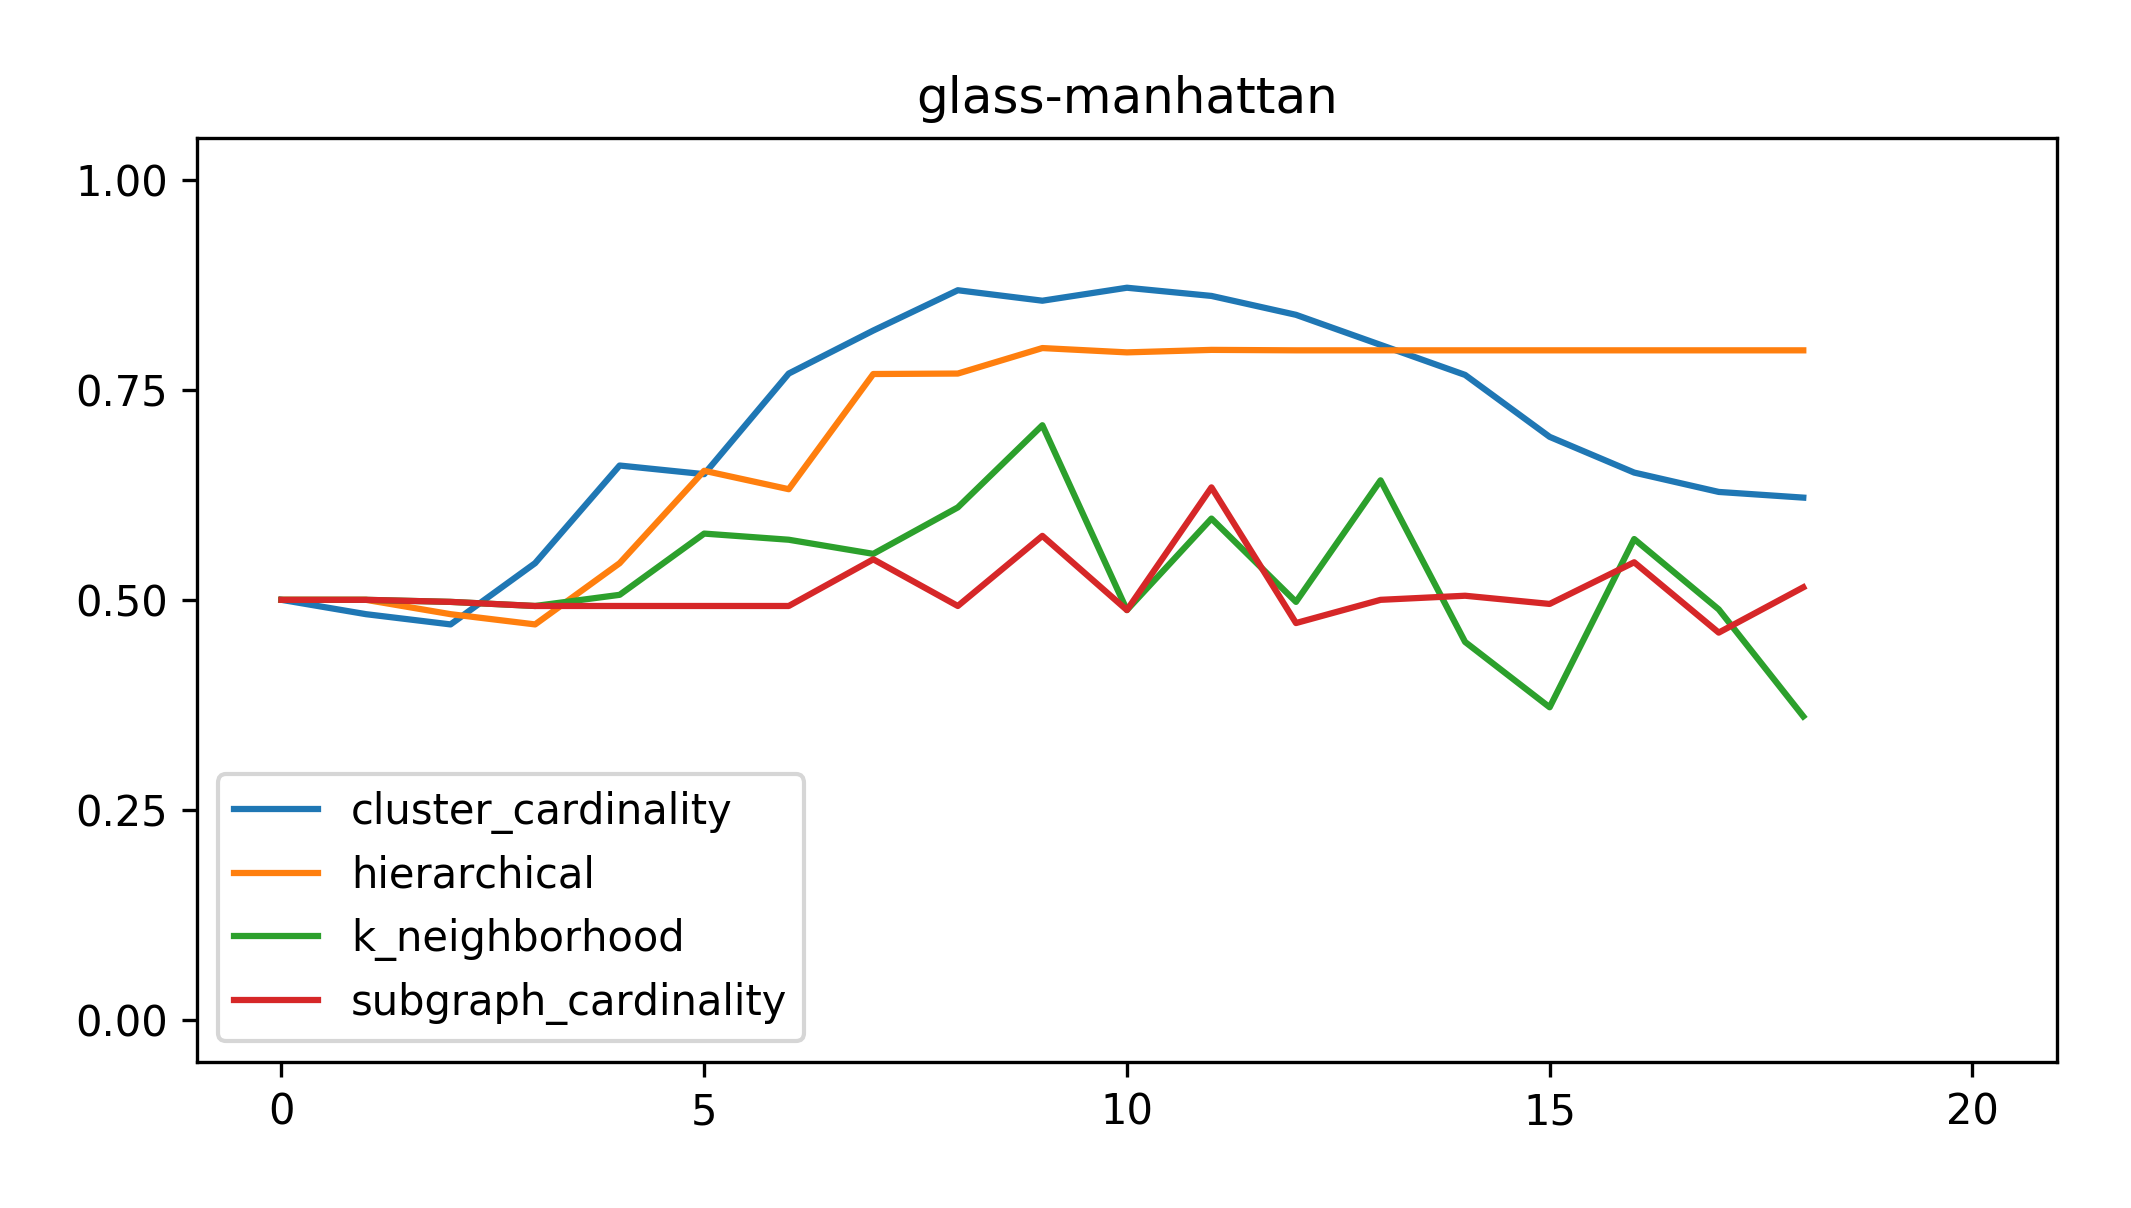
\includegraphics[width=2.2in]{kdd/static/auc_vs_depth/glass-manhattan.png}

% Ionosphere
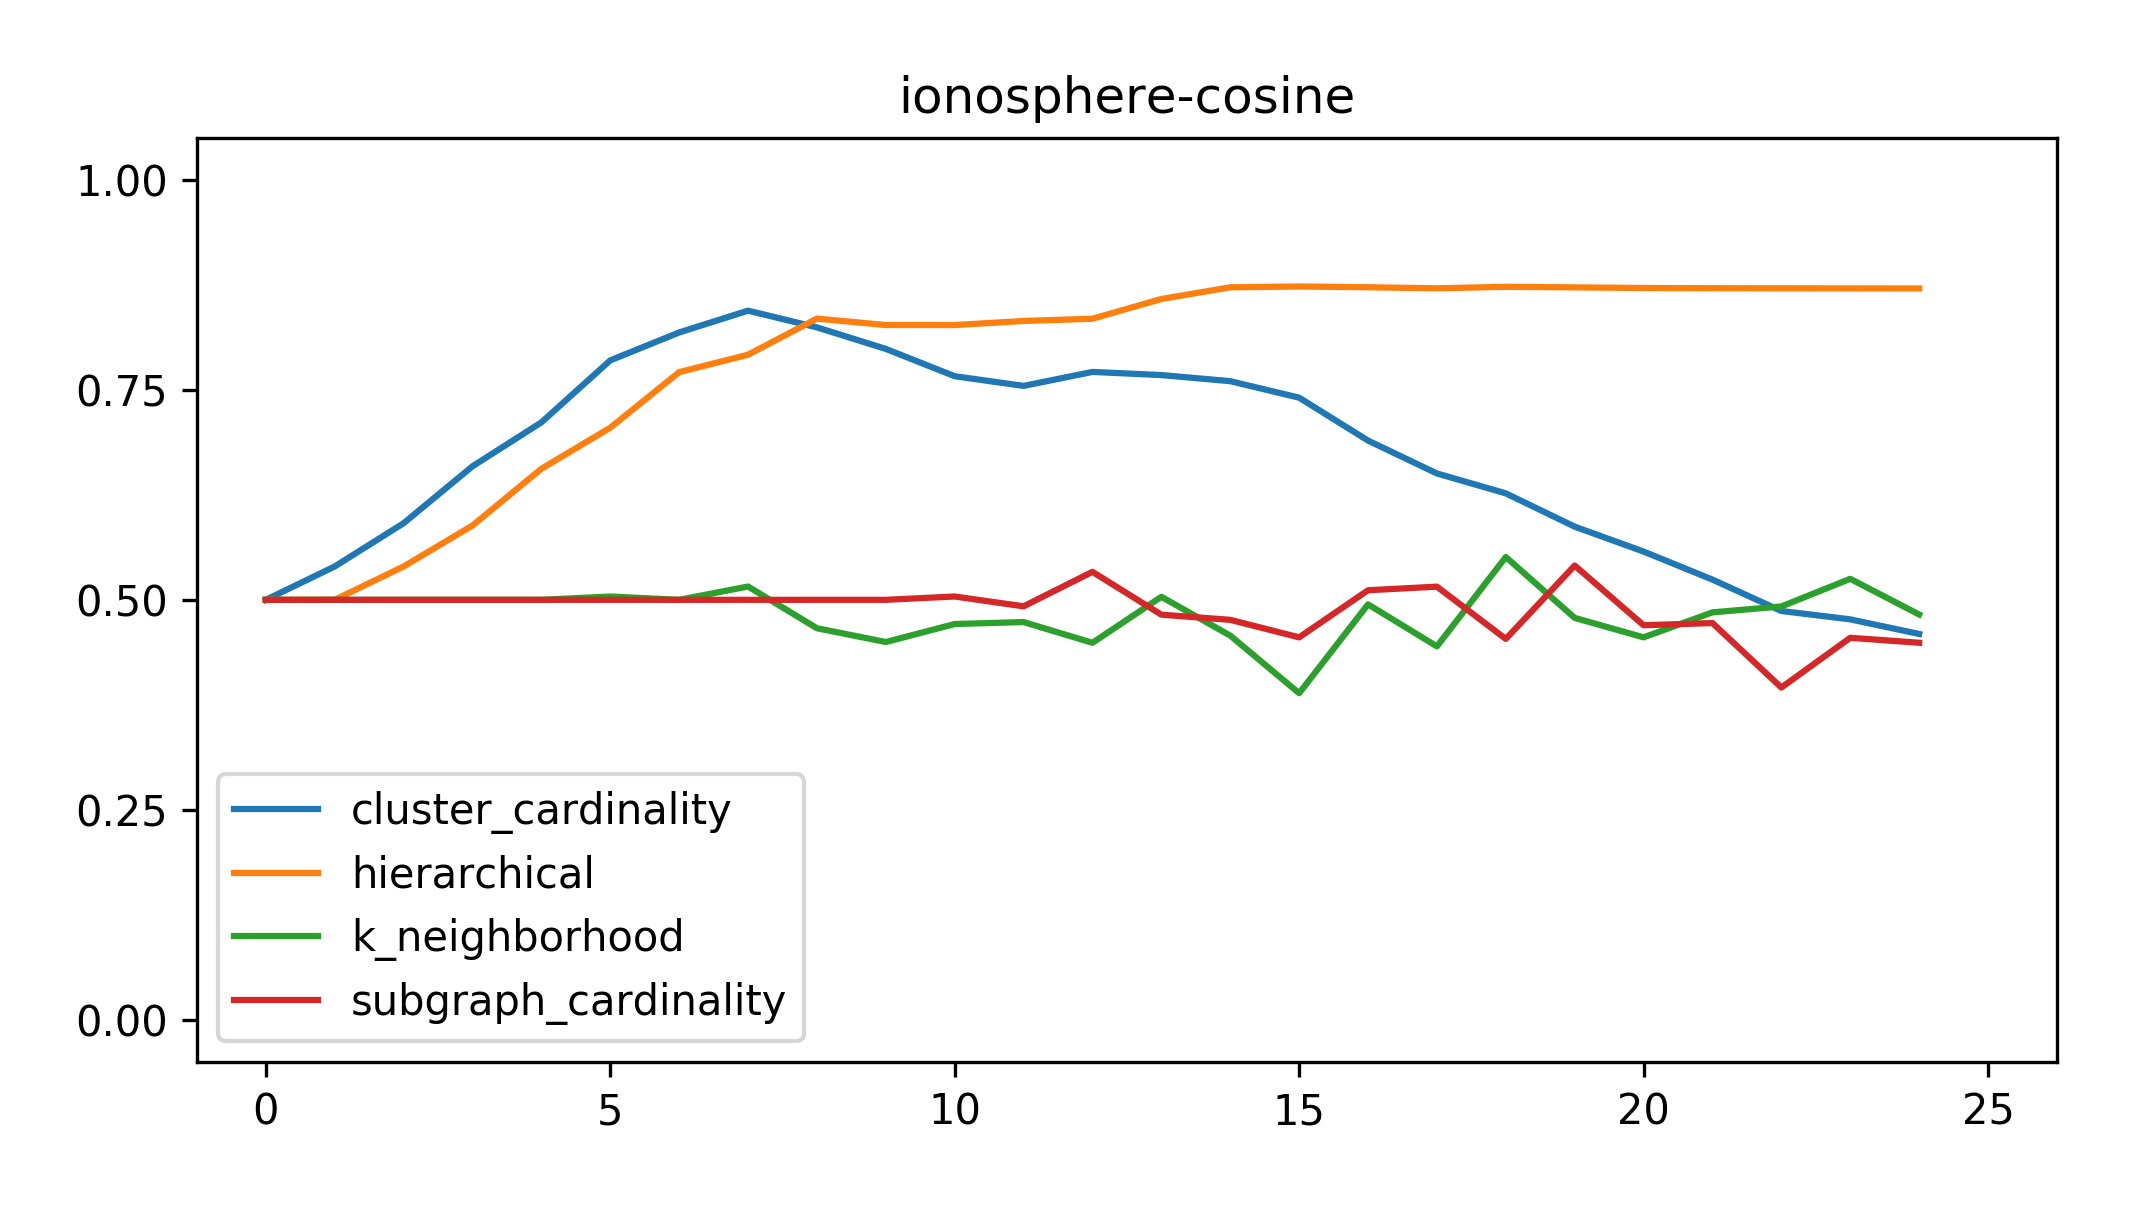
\includegraphics[width=2.2in]{kdd/static/auc_vs_depth/ionosphere-cosine.png}
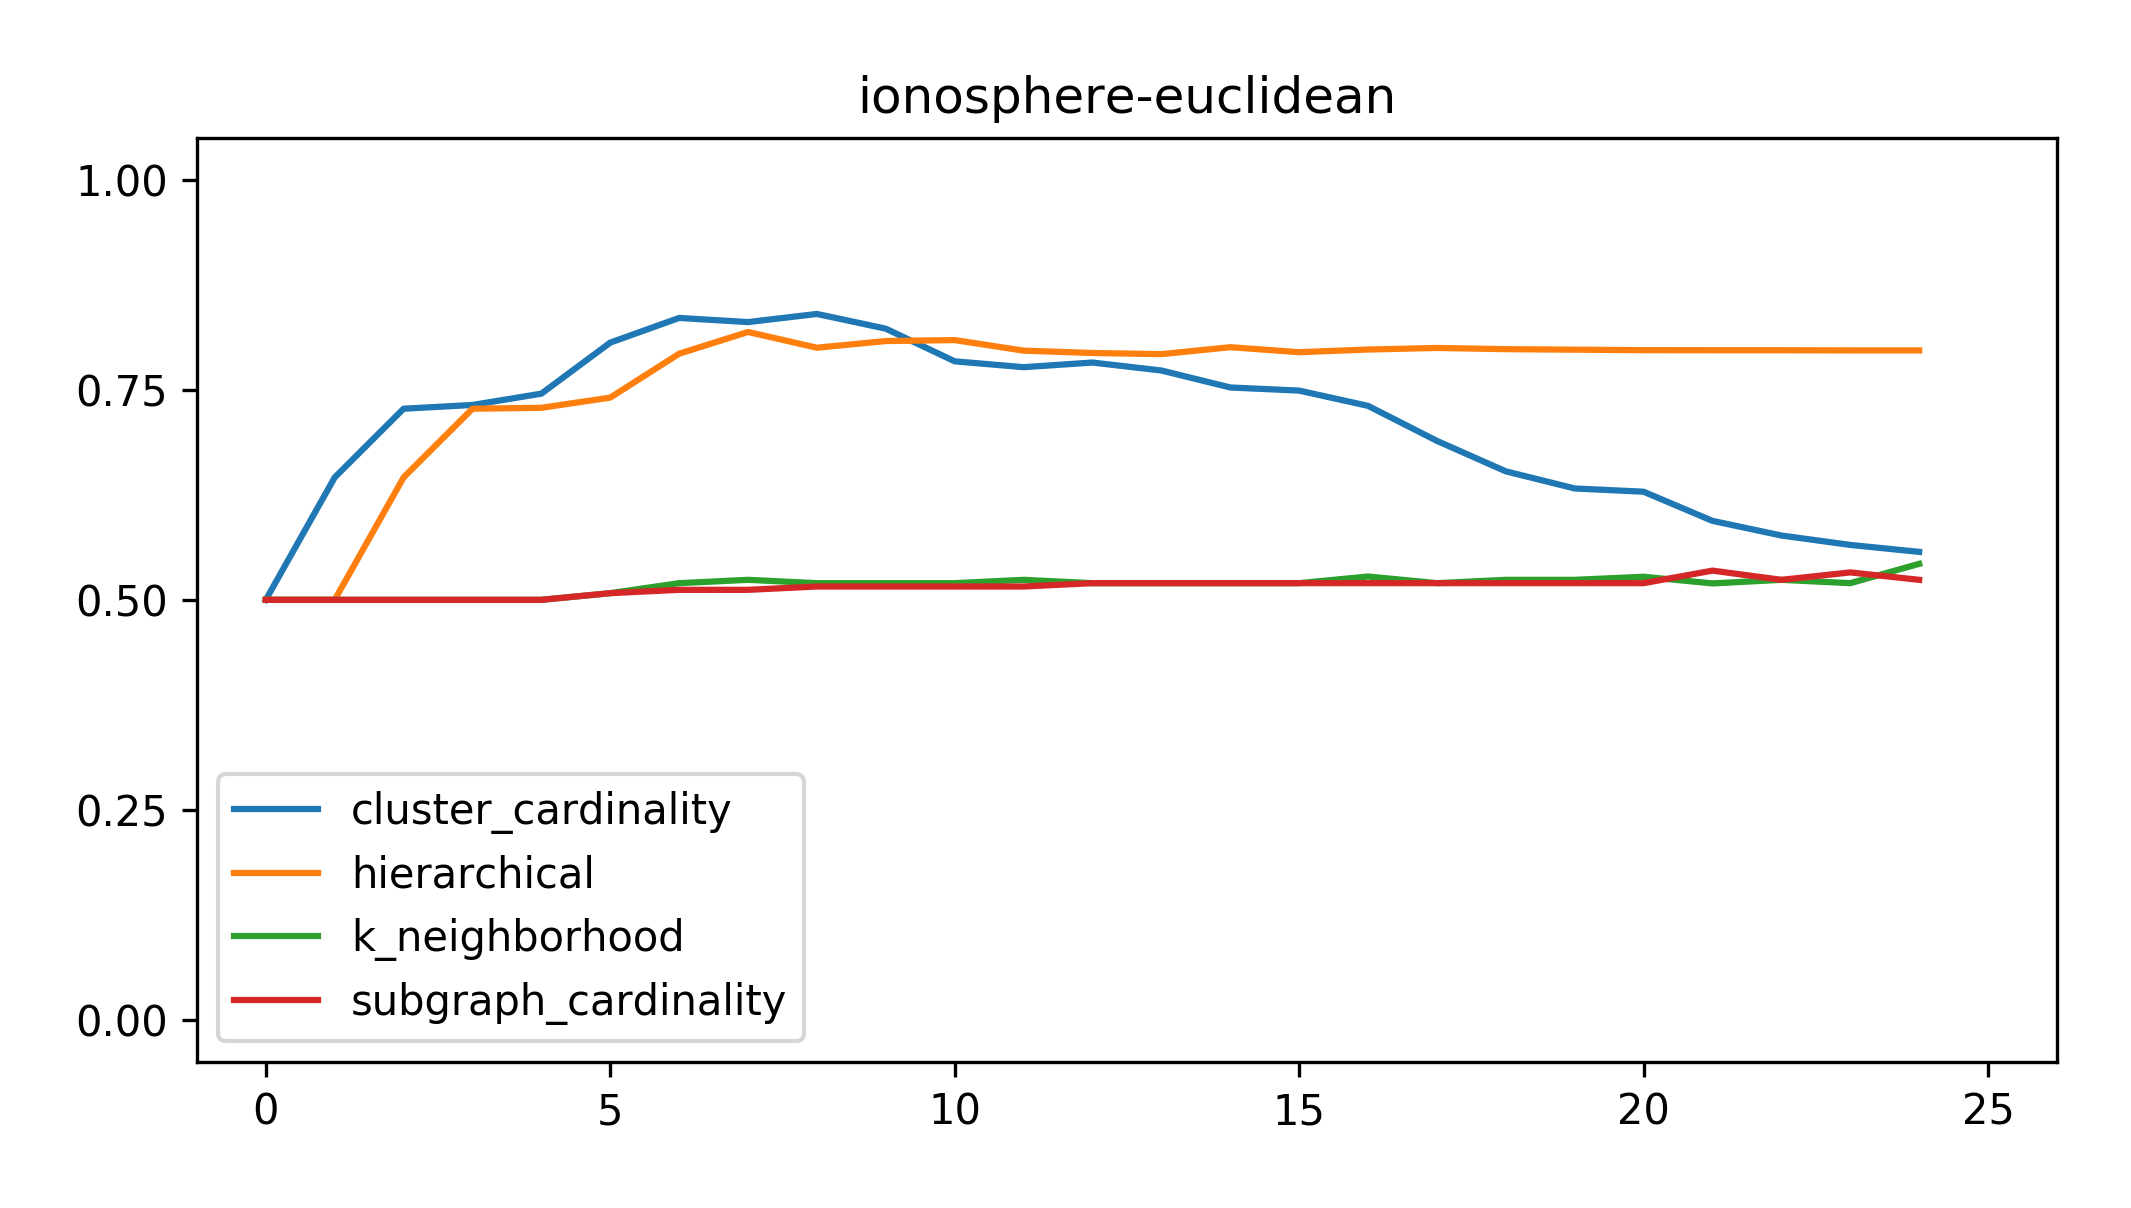
\includegraphics[width=2.2in]{kdd/static/auc_vs_depth/ionosphere-euclidean.png}
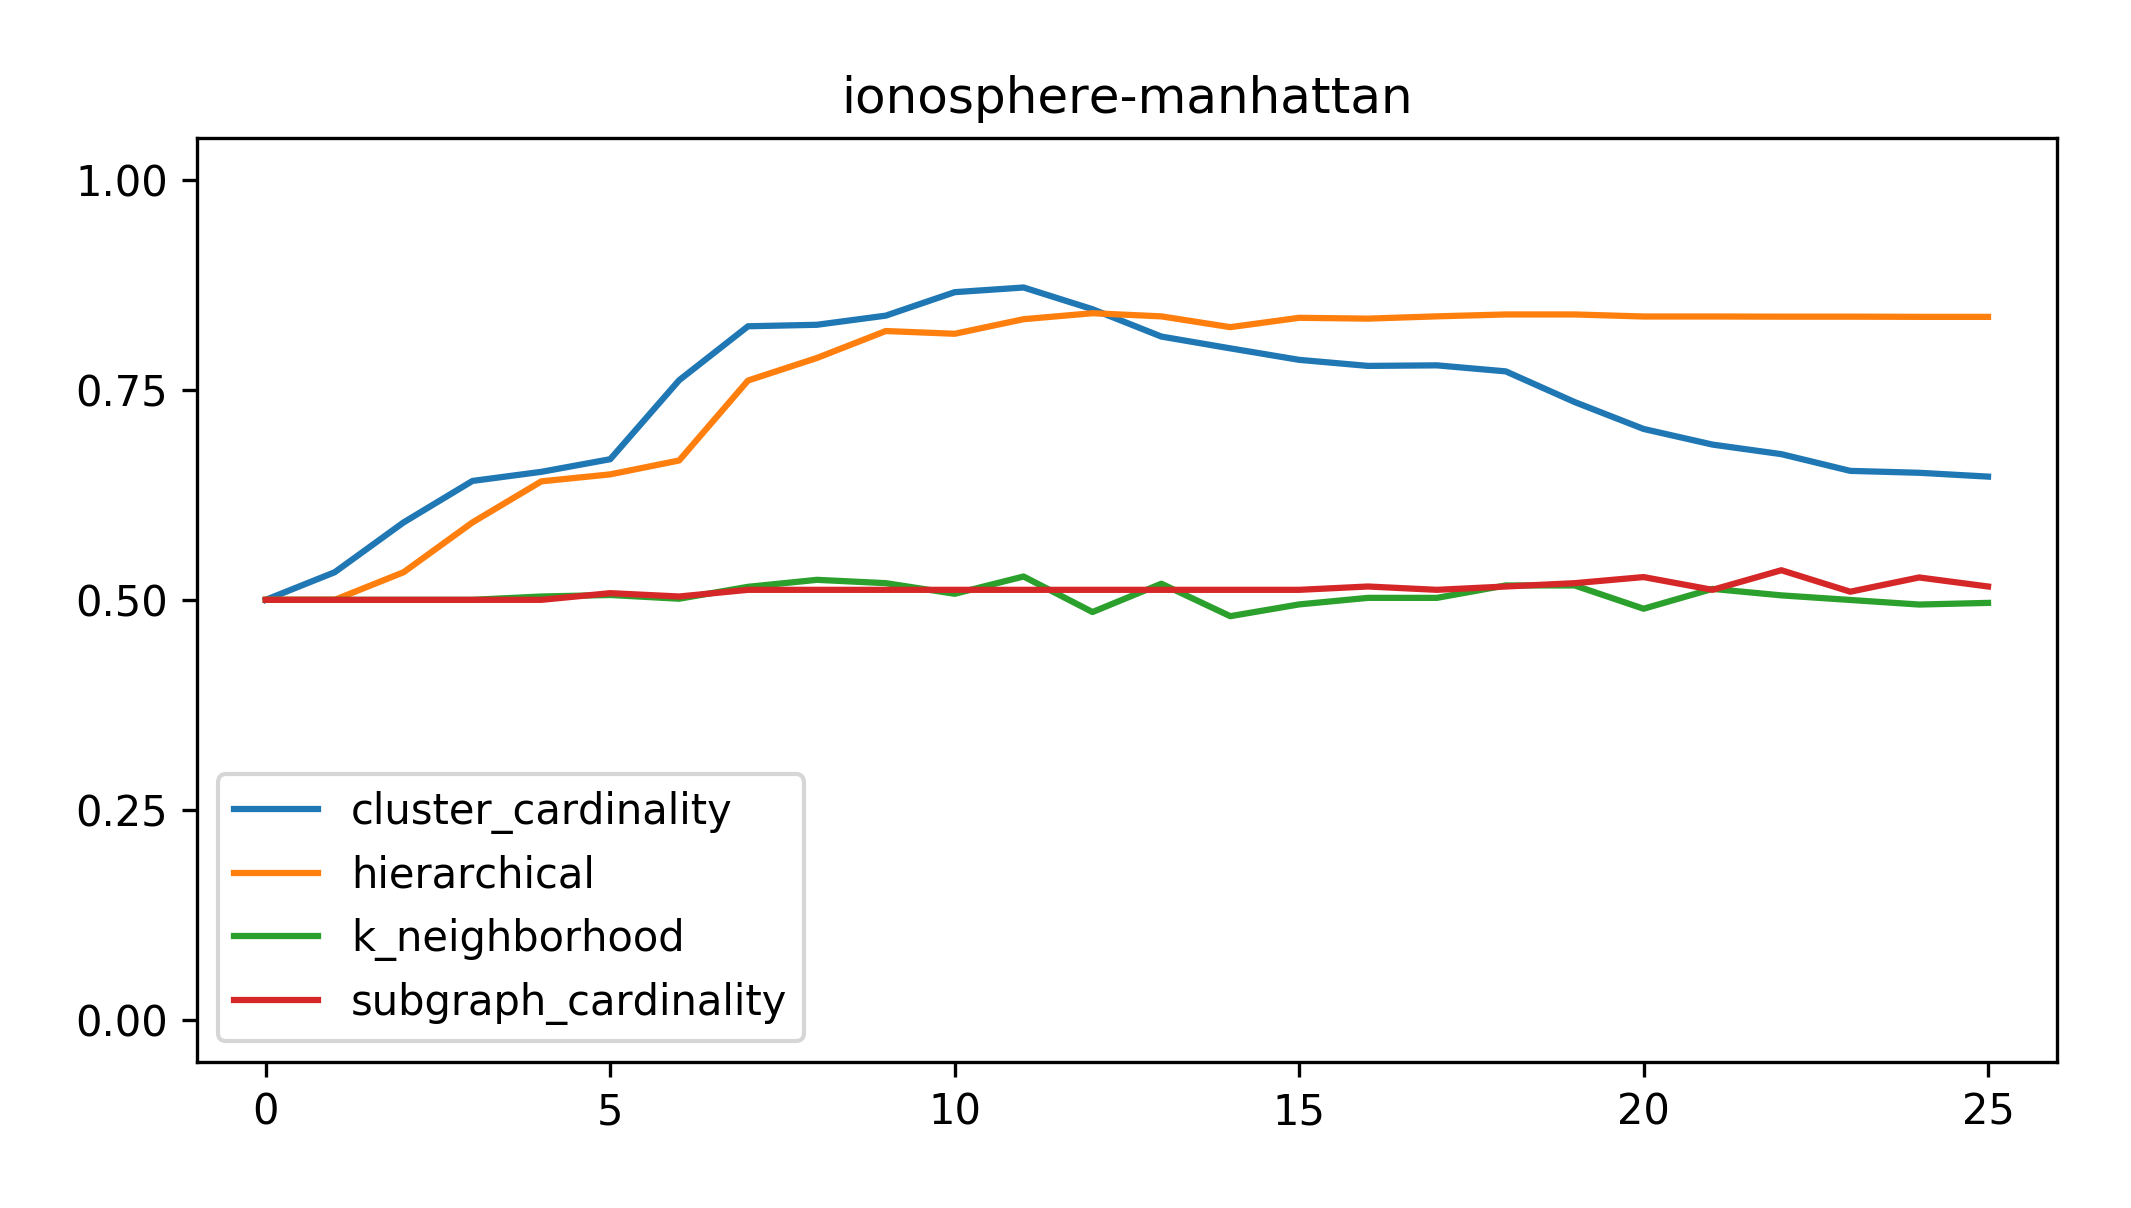
\includegraphics[width=2.2in]{kdd/static/auc_vs_depth/ionosphere-manhattan.png}

\caption{
Plots of ROC-AUC vs Depth for our mearures of Anomolousness.
}

\label{results:datasets_1}
\end{figure*}

\begin{figure*}[!t]
\centering
% Lympho
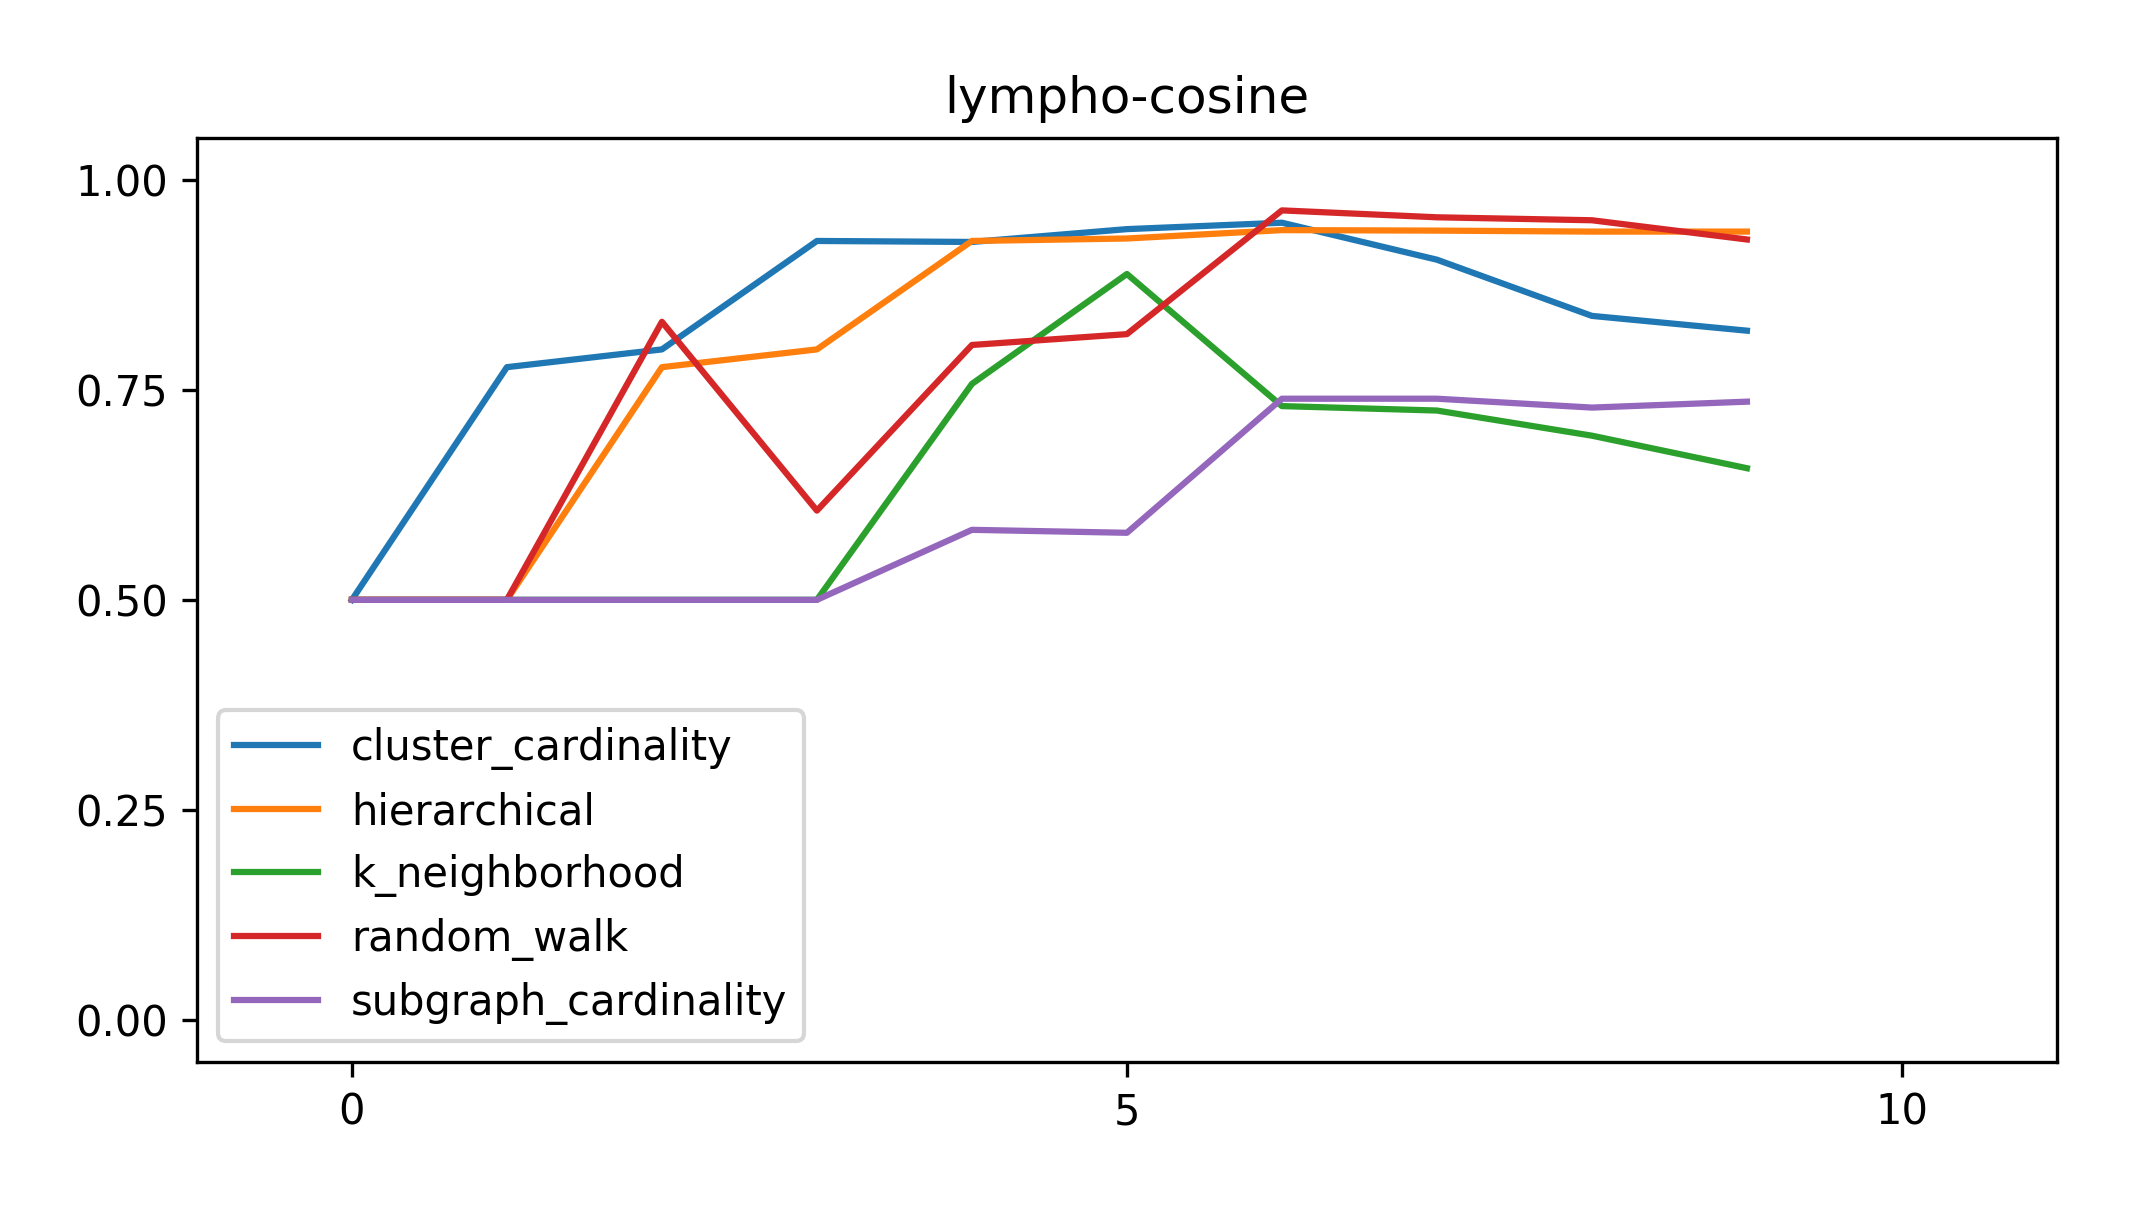
\includegraphics[width=2.2in]{kdd/static/auc_vs_depth/lympho-cosine.png}
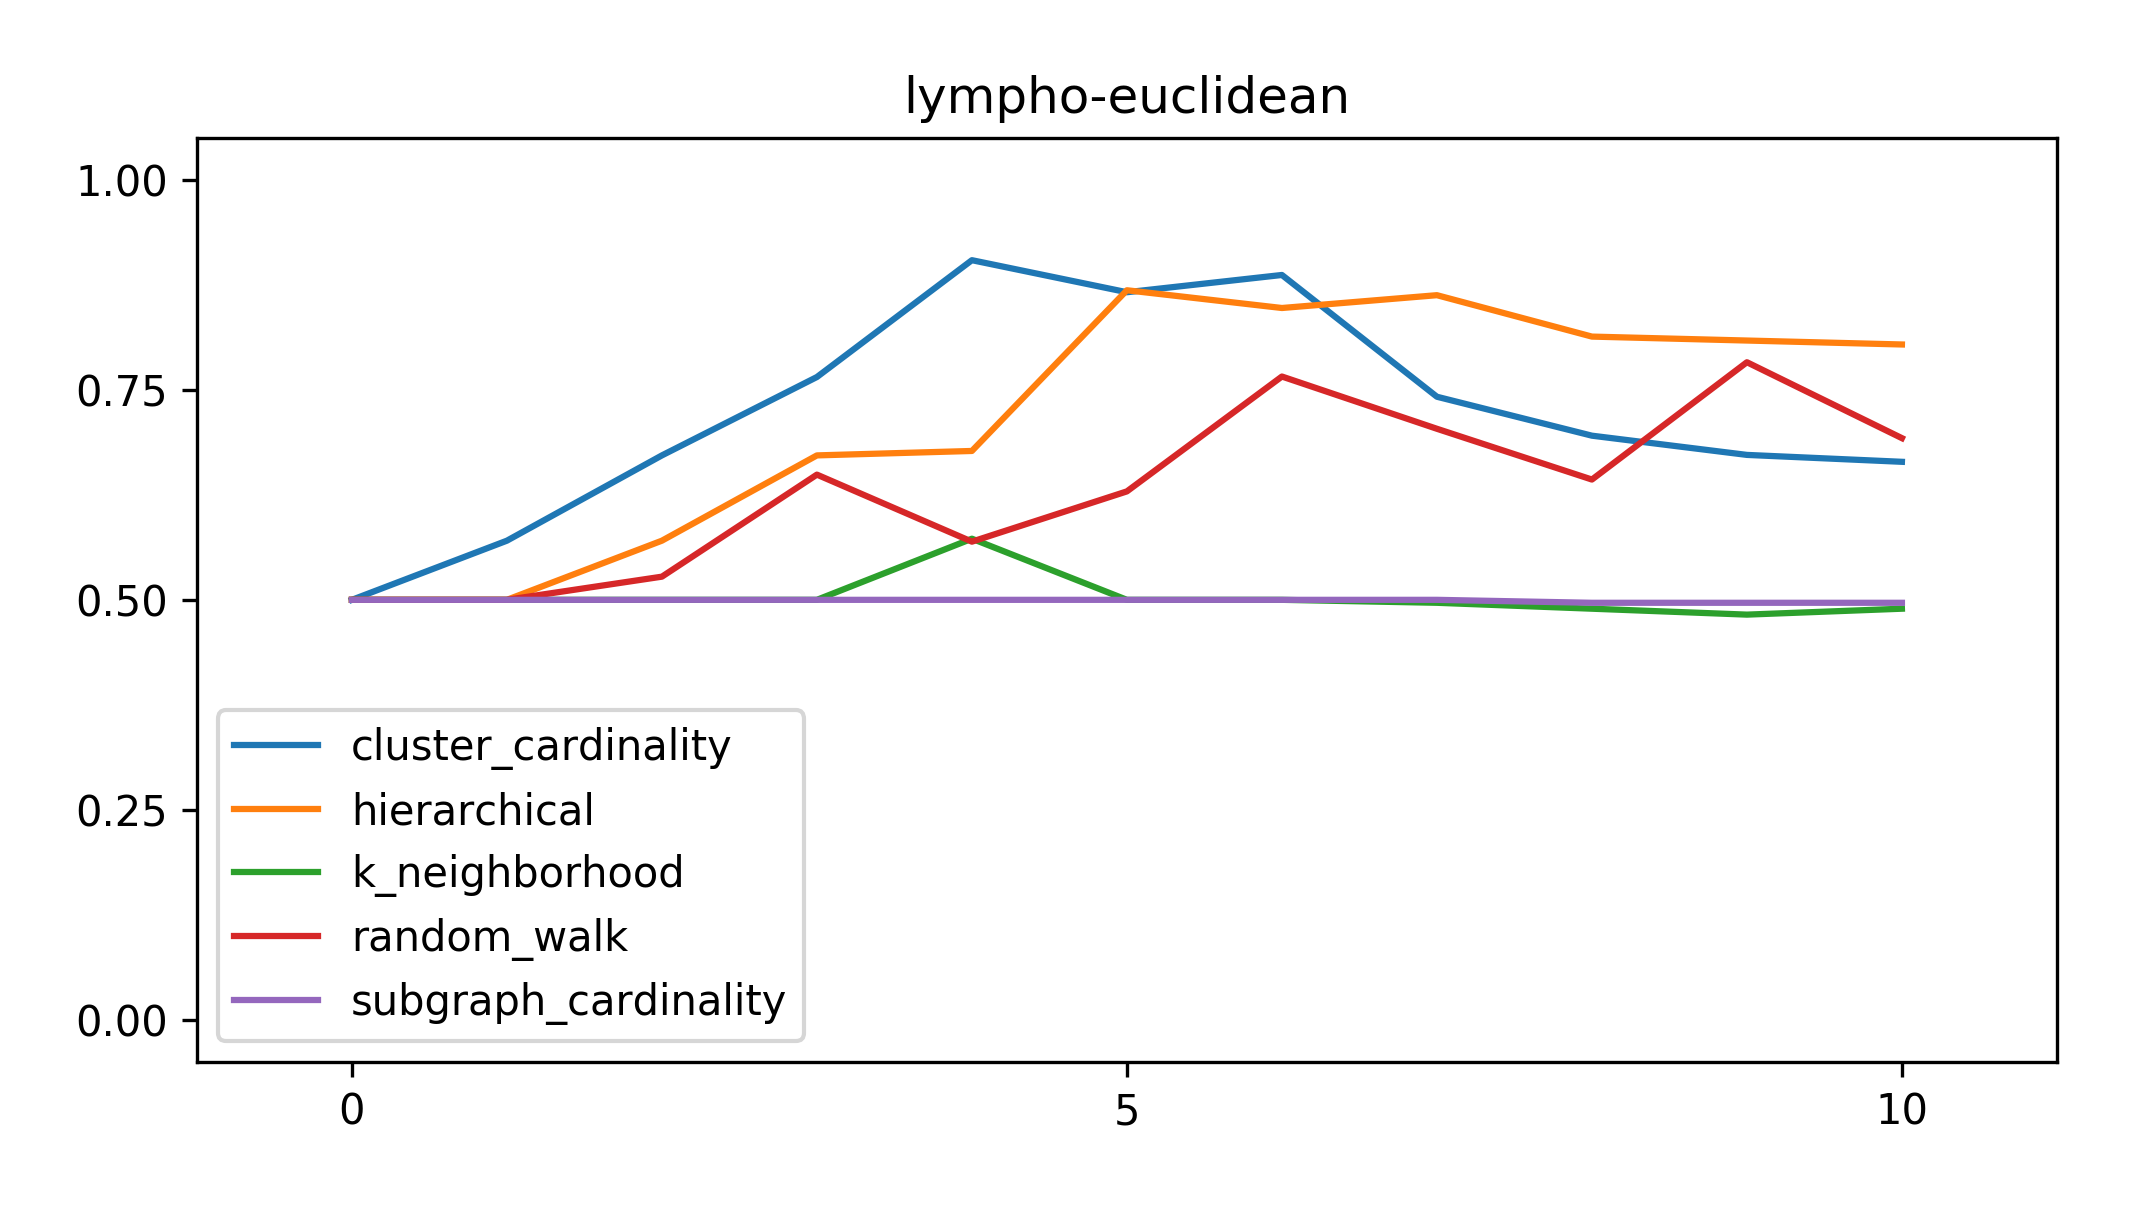
\includegraphics[width=2.2in]{kdd/static/auc_vs_depth/lympho-euclidean.png}
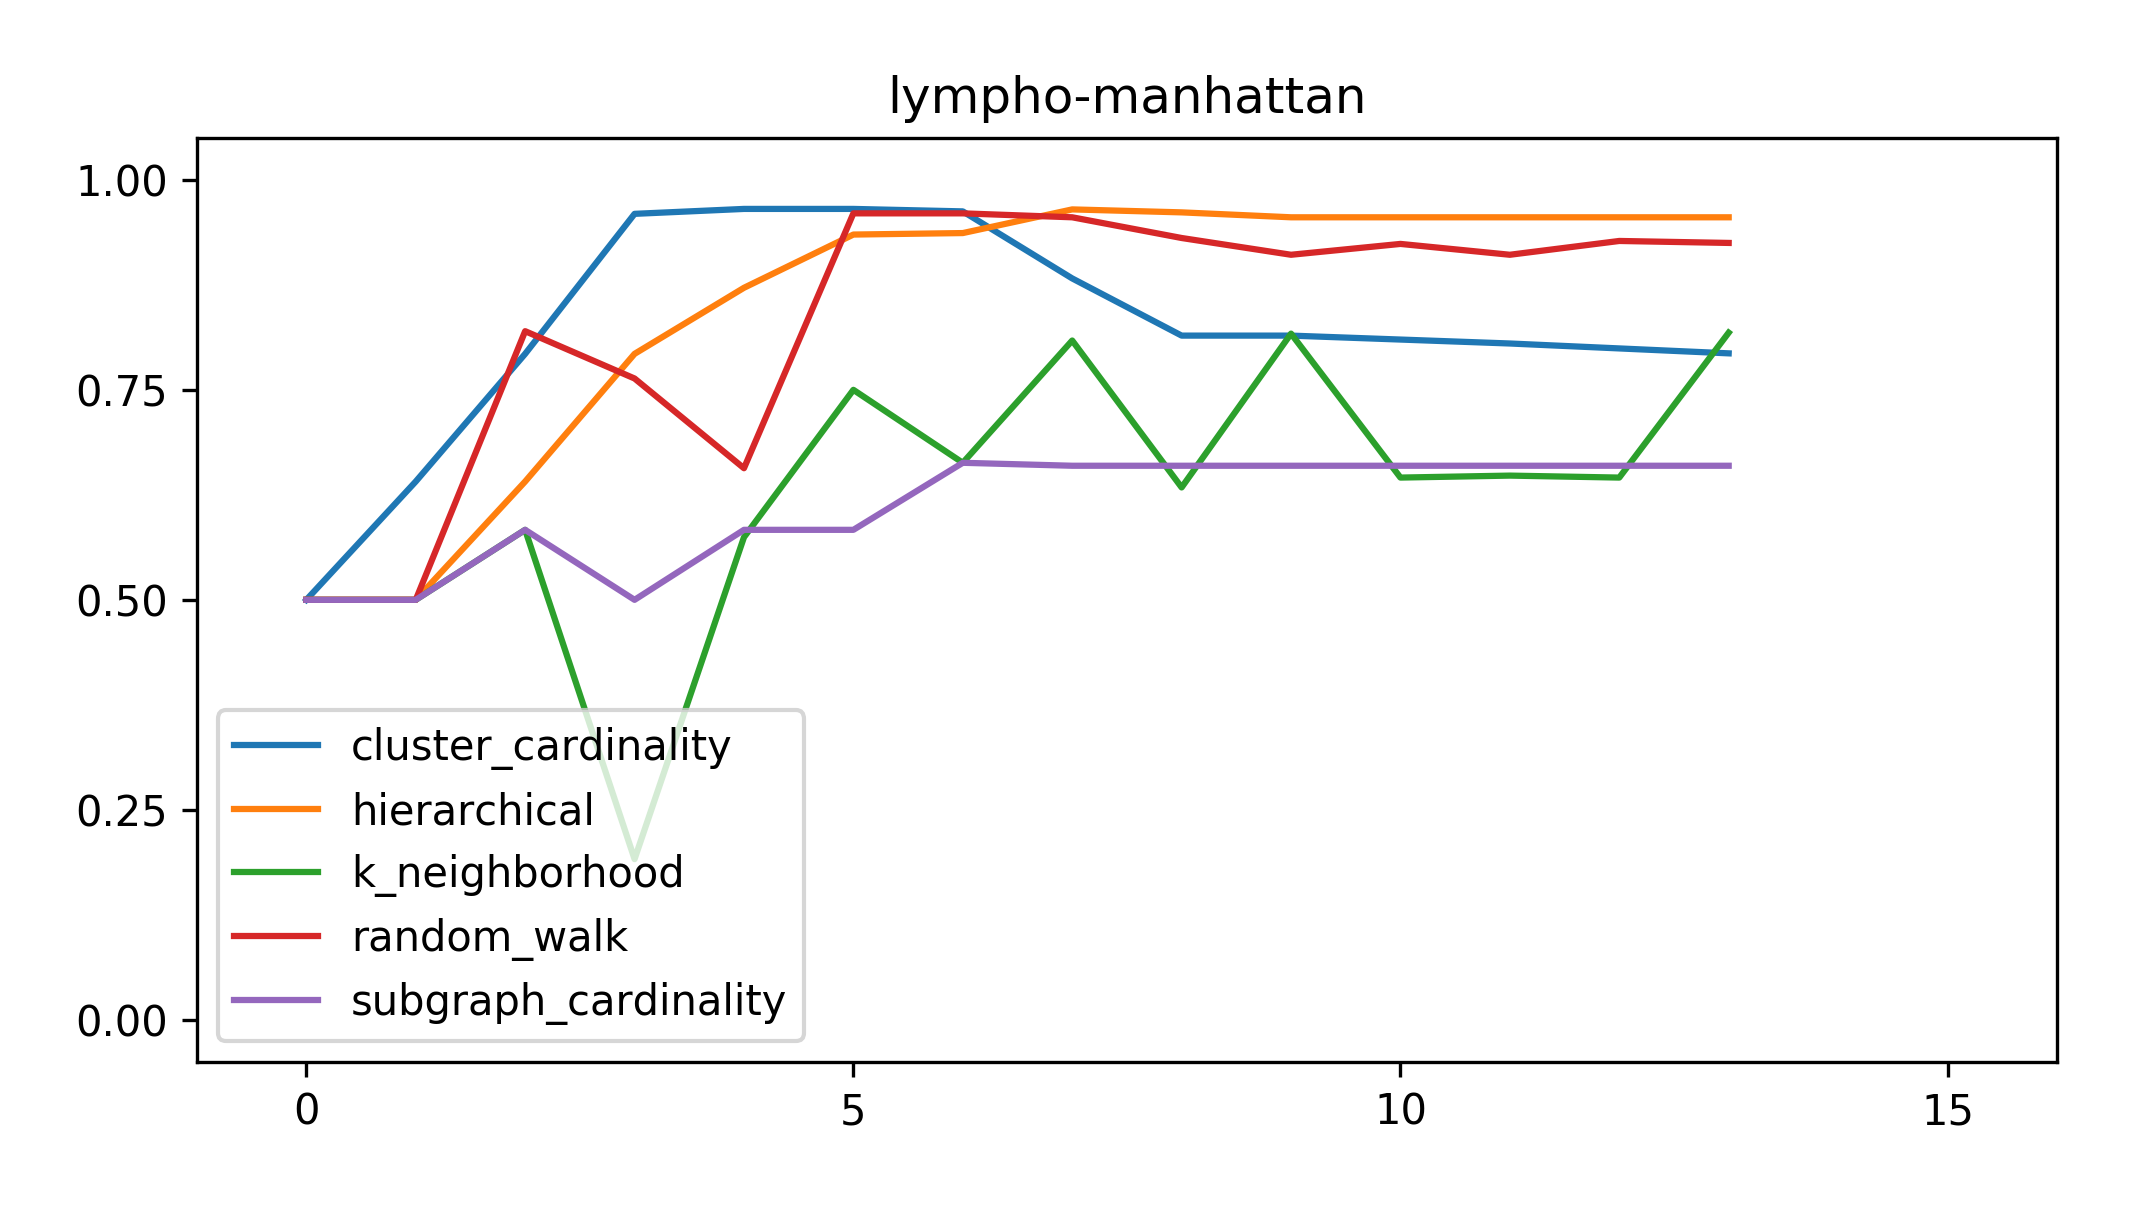
\includegraphics[width=2.2in]{kdd/static/auc_vs_depth/lympho-manhattan.png}

% Mnist
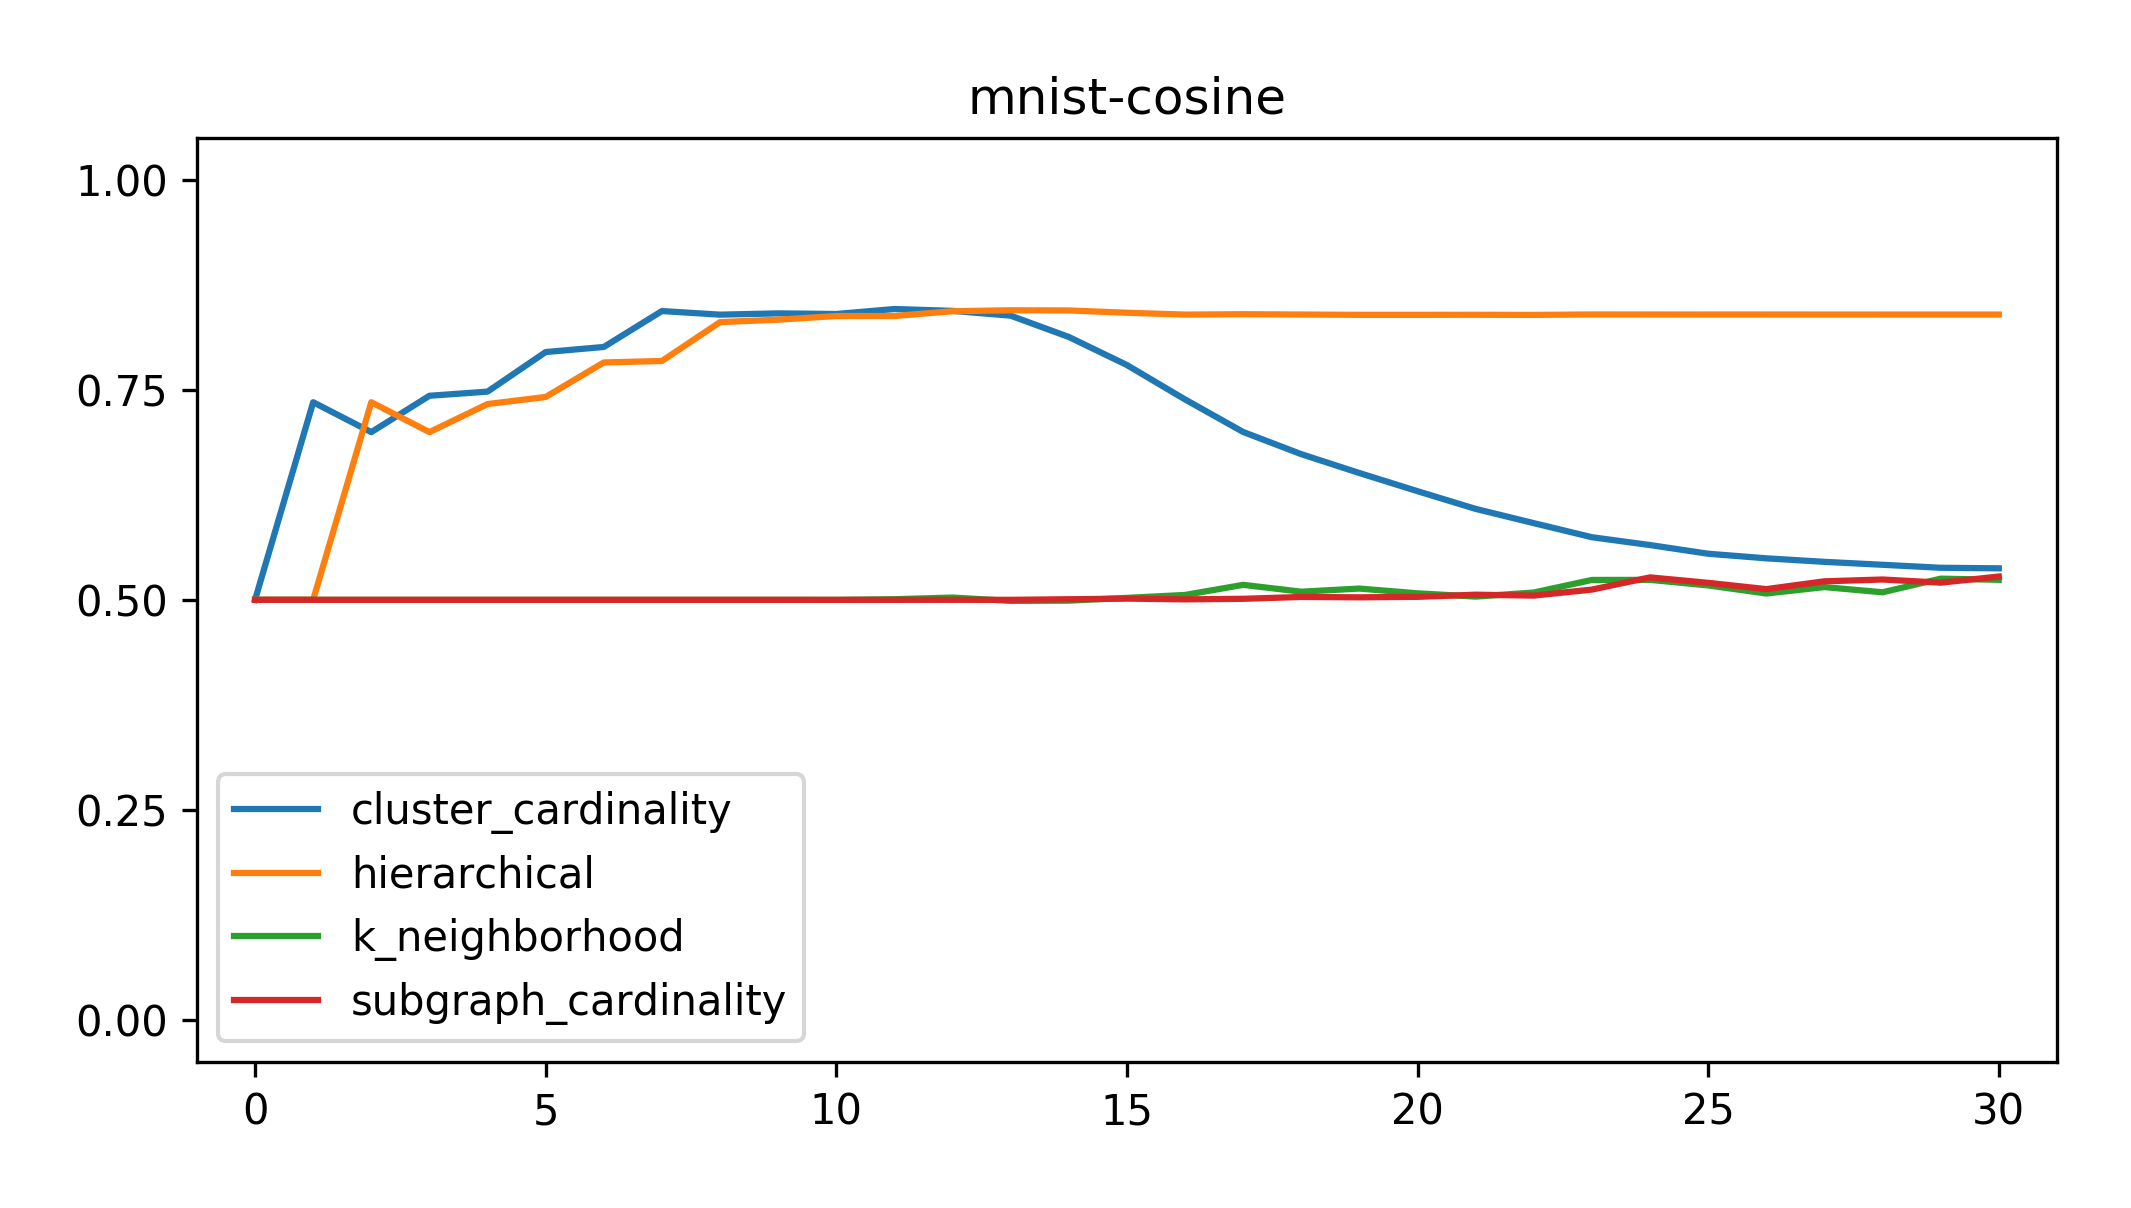
\includegraphics[width=2.2in]{kdd/static/auc_vs_depth/mnist-cosine.png}
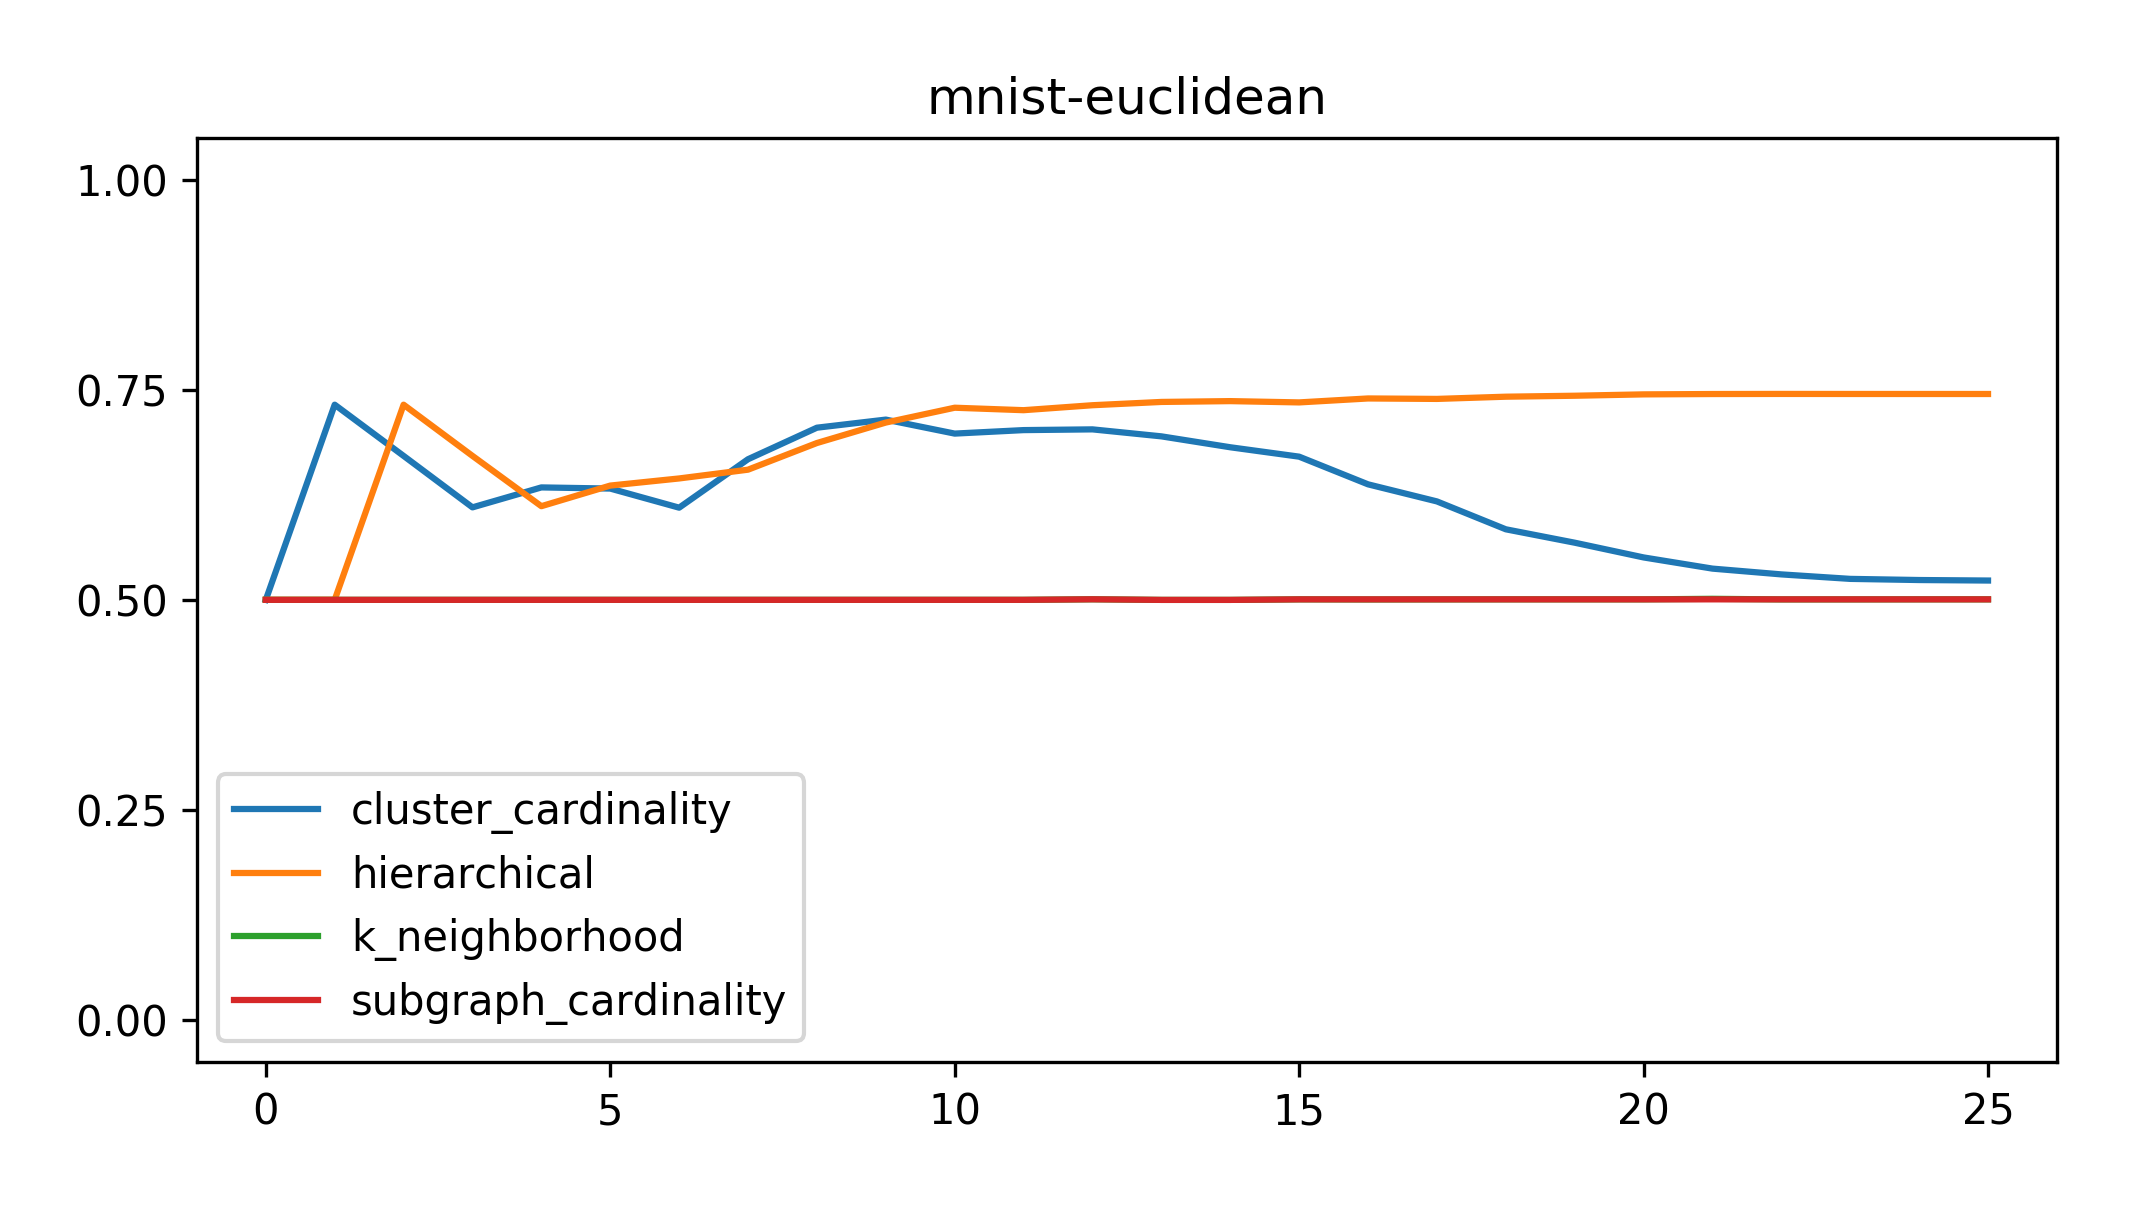
\includegraphics[width=2.2in]{kdd/static/auc_vs_depth/mnist-euclidean.png}
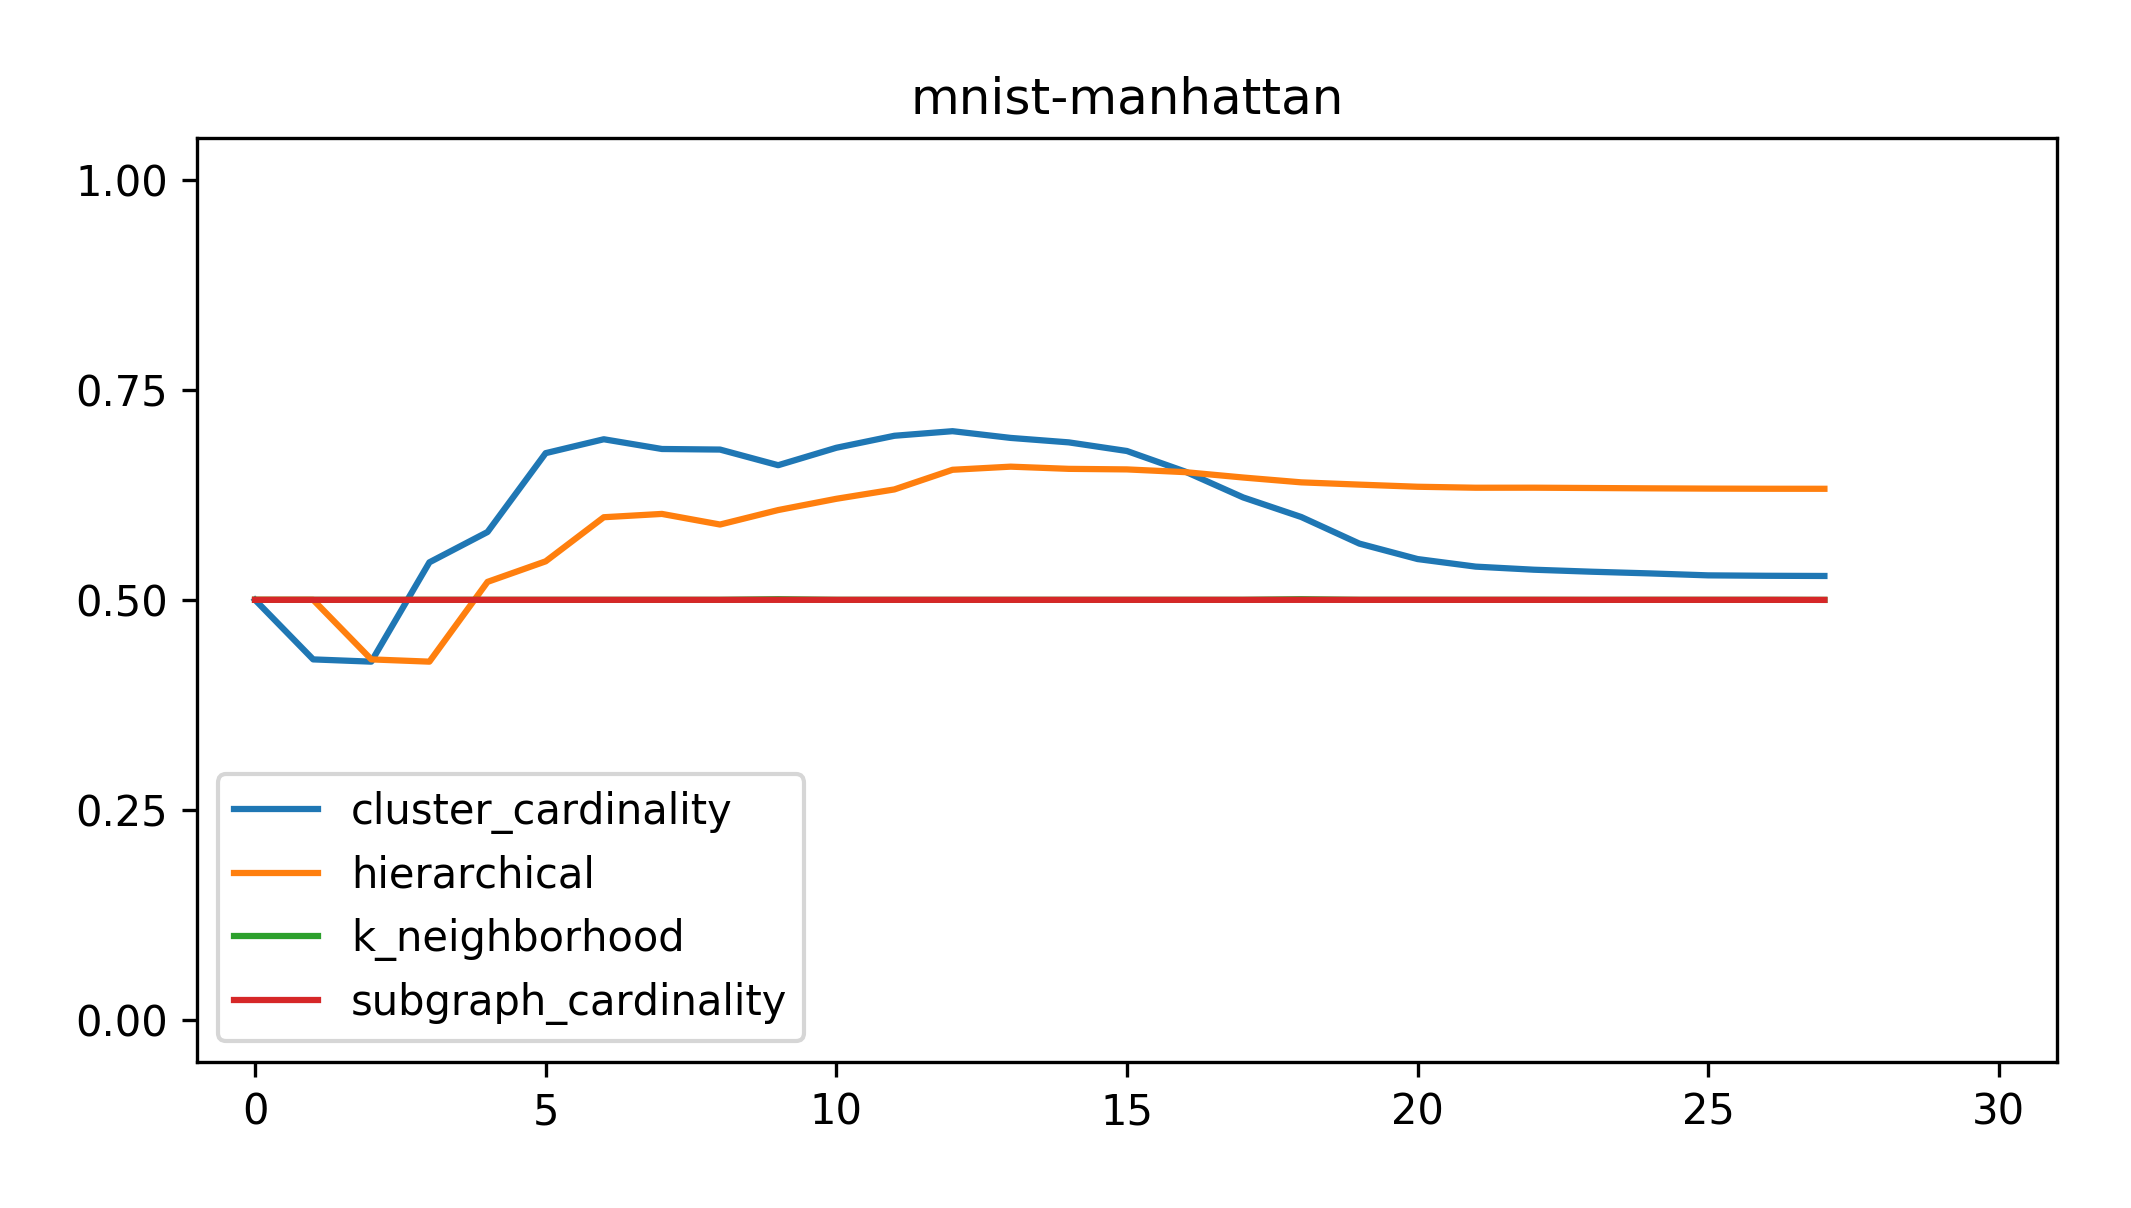
\includegraphics[width=2.2in]{kdd/static/auc_vs_depth/mnist-manhattan.png}

% Musk
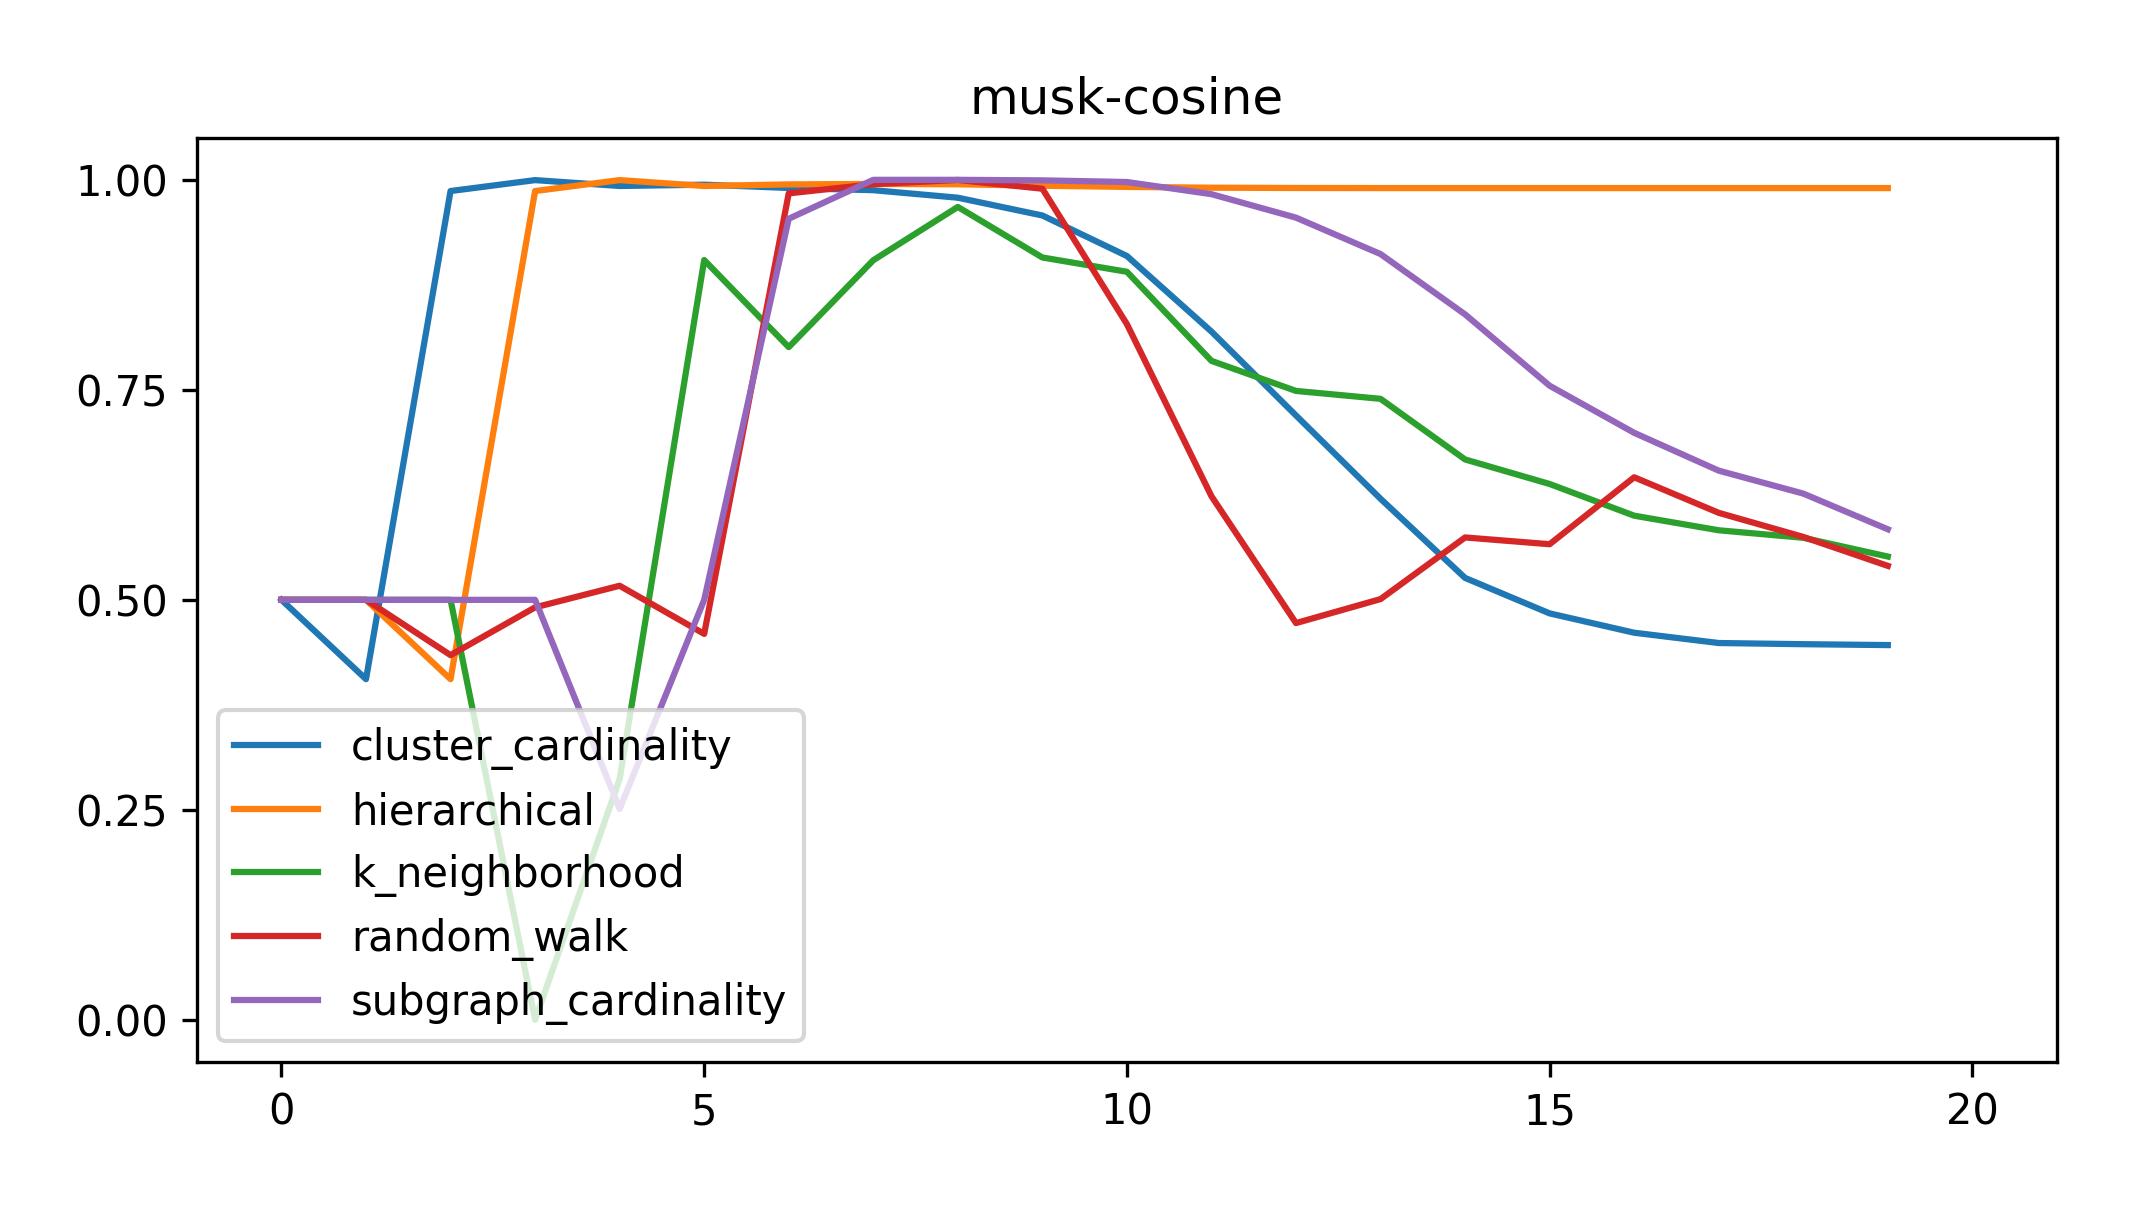
\includegraphics[width=2.2in]{kdd/static/auc_vs_depth/musk-cosine.png}
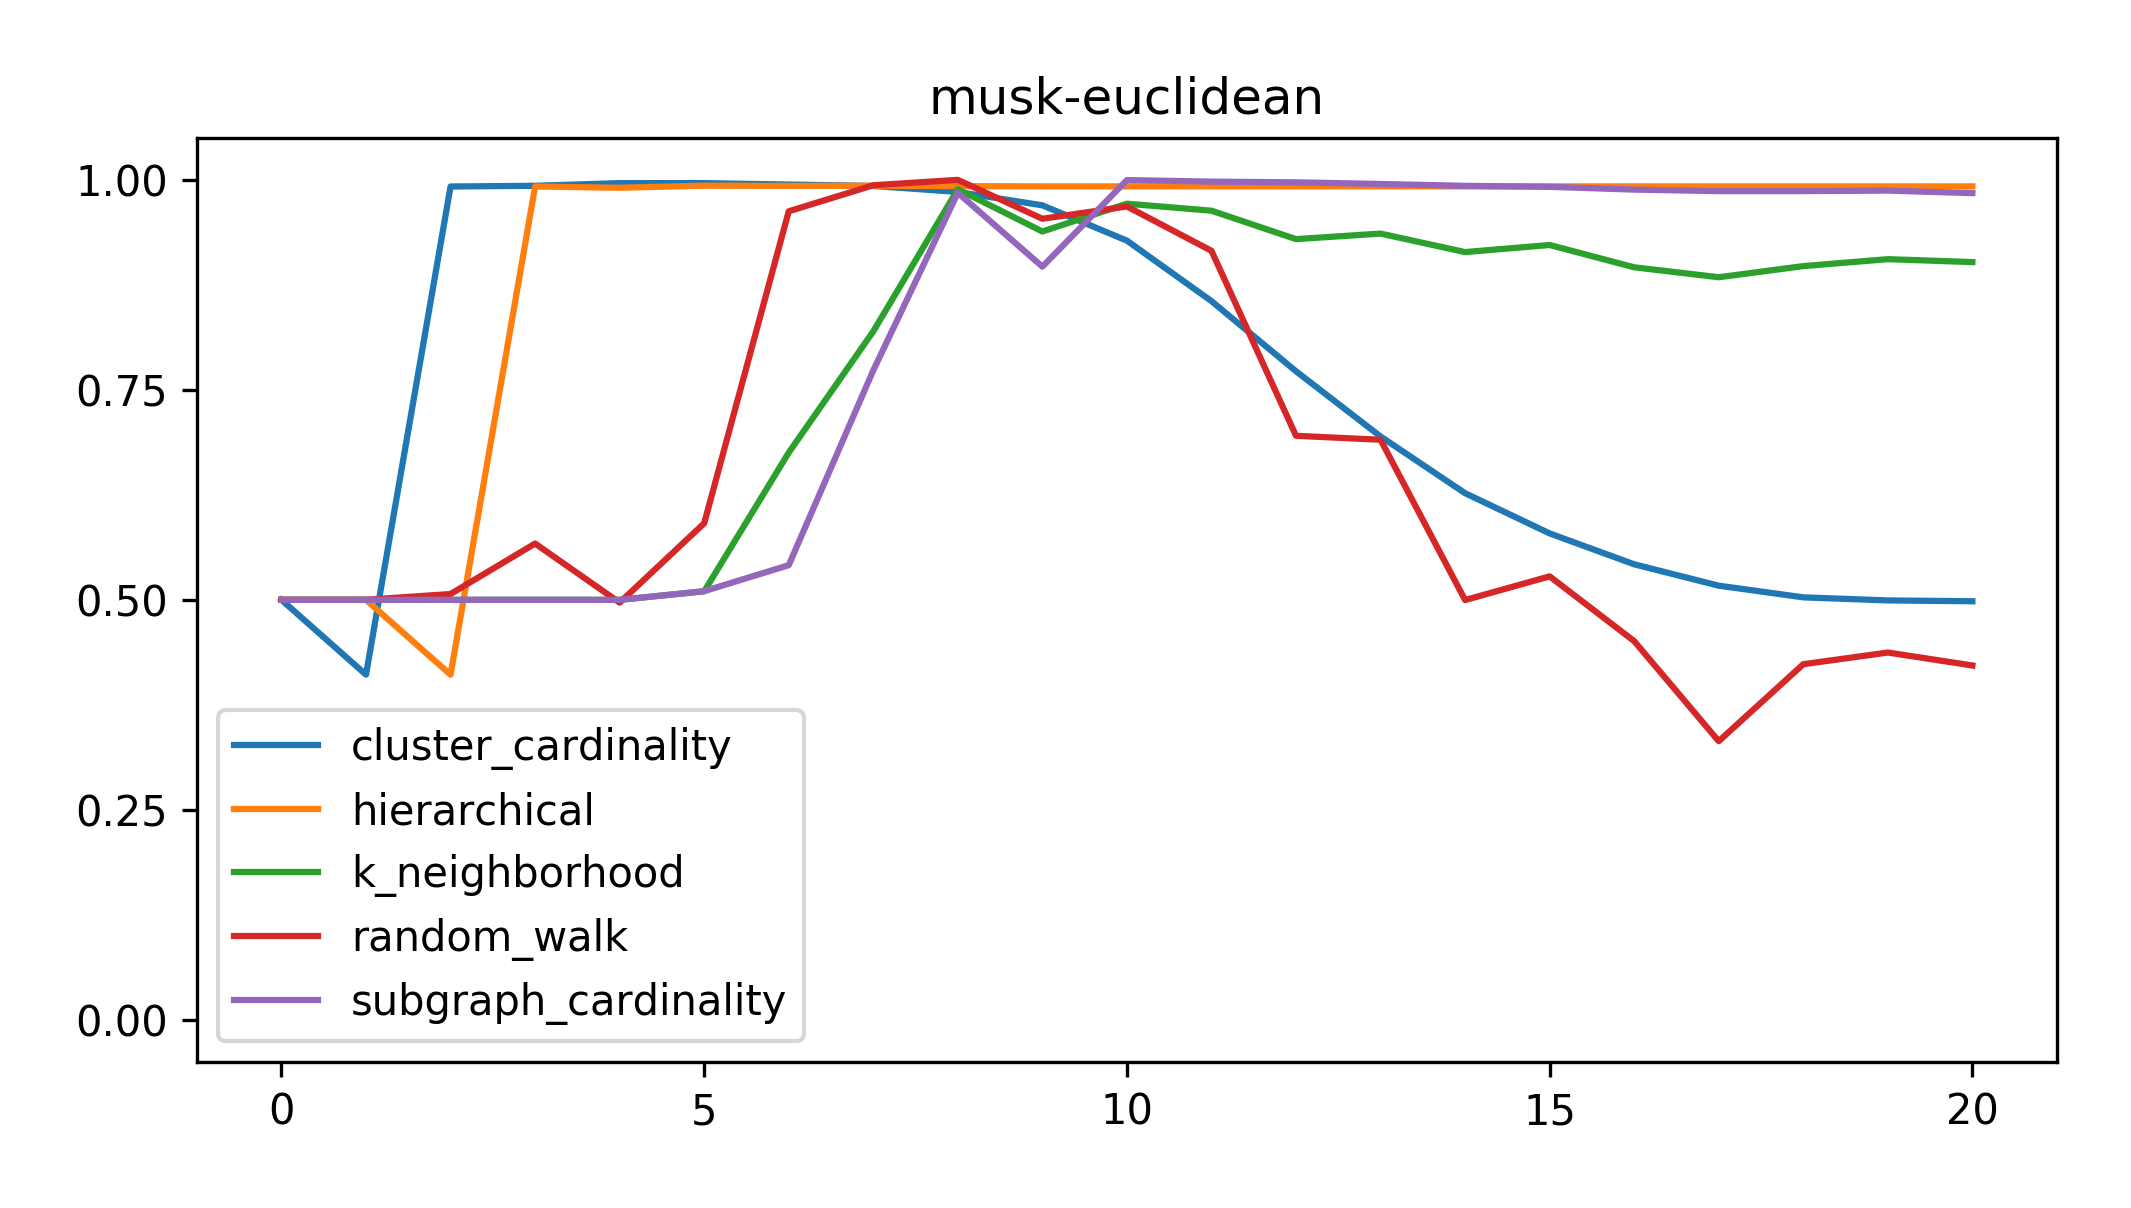
\includegraphics[width=2.2in]{kdd/static/auc_vs_depth/musk-euclidean.png}
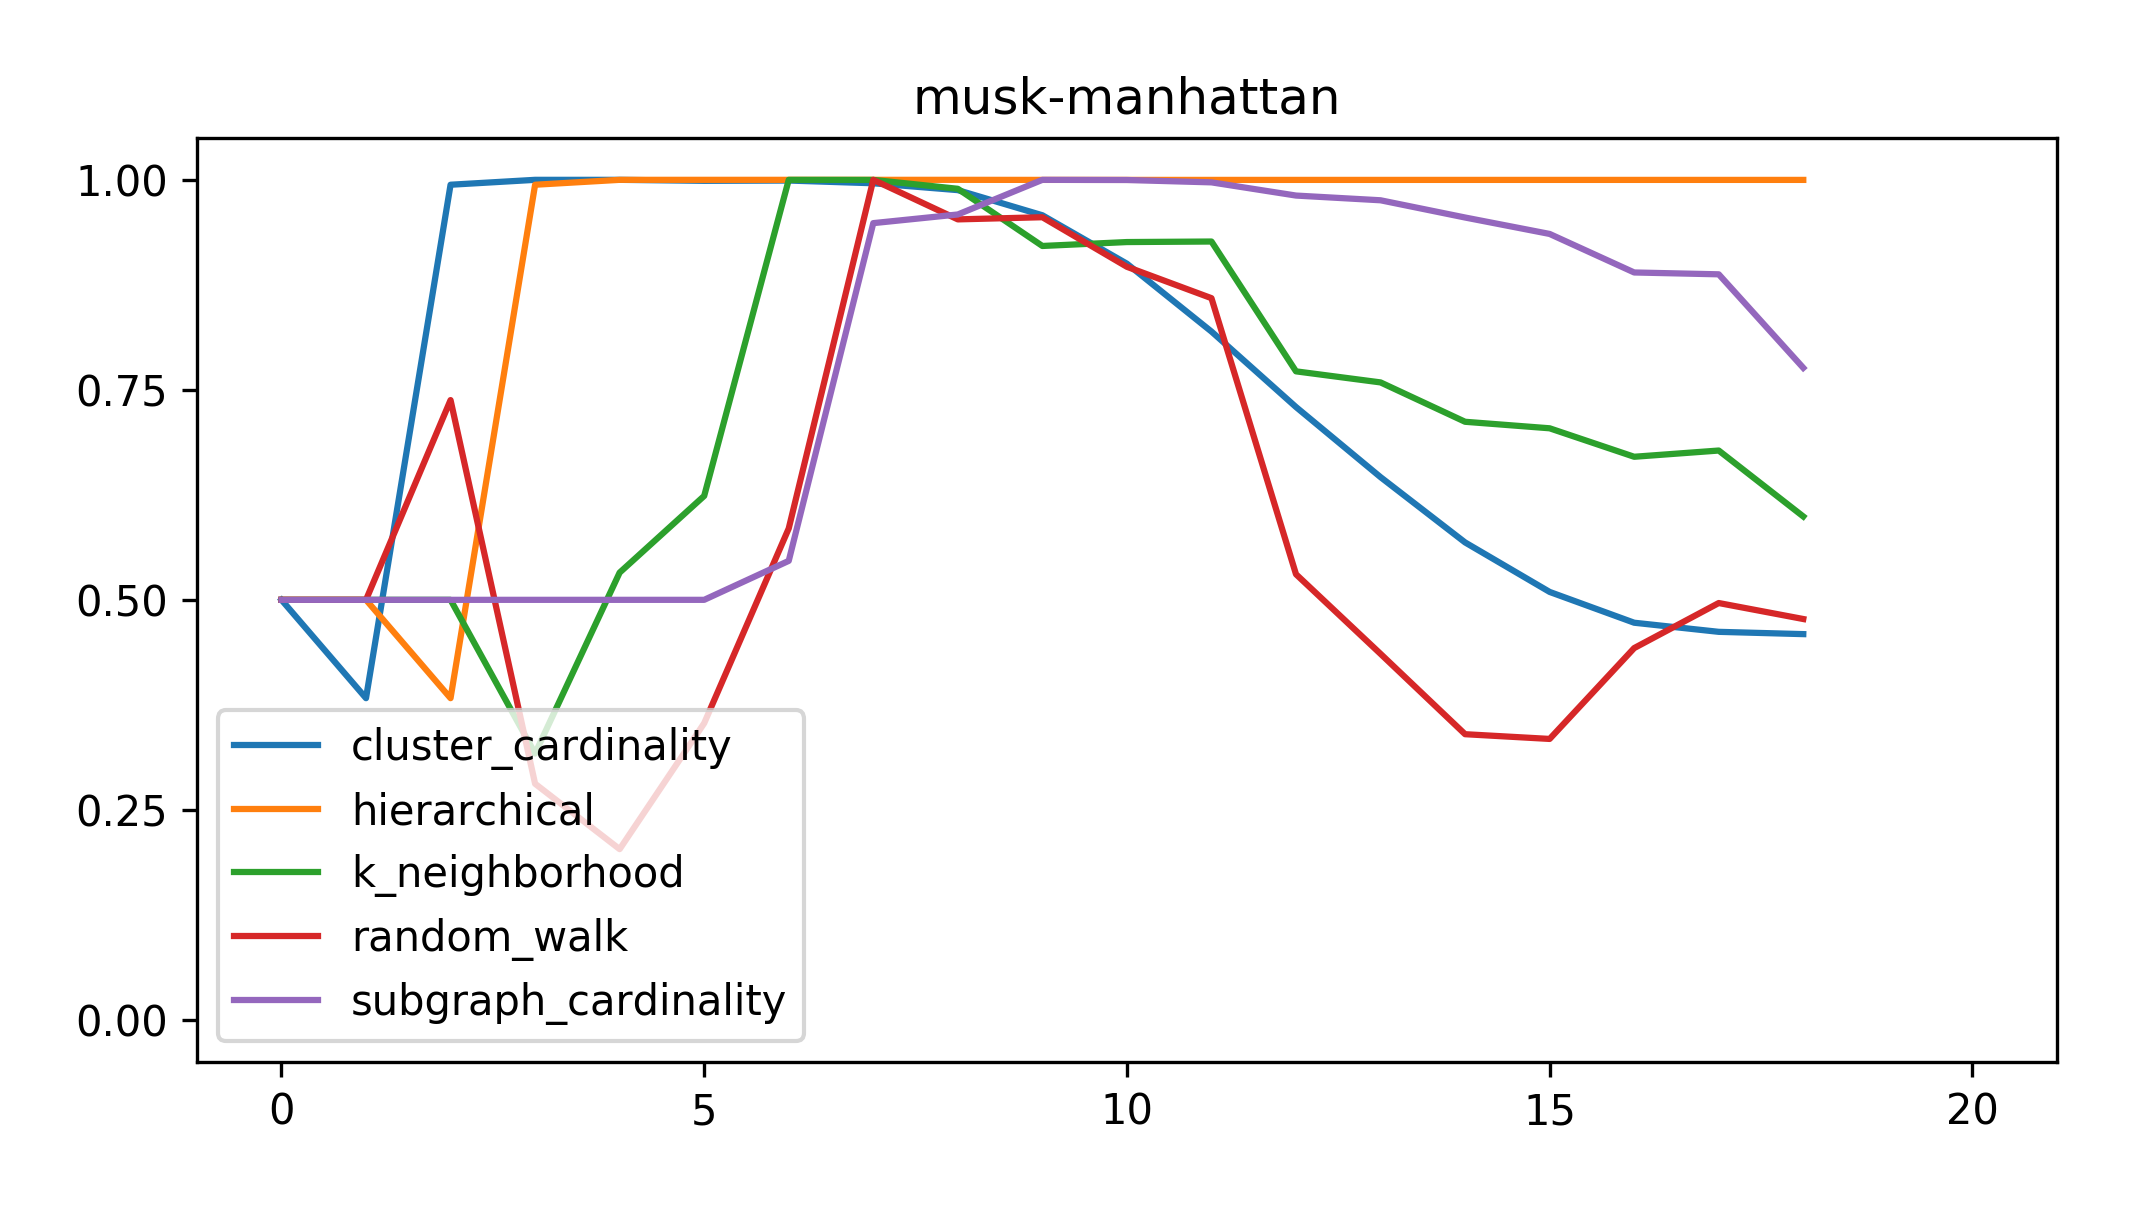
\includegraphics[width=2.2in]{kdd/static/auc_vs_depth/musk-manhattan.png}

% Optdigits
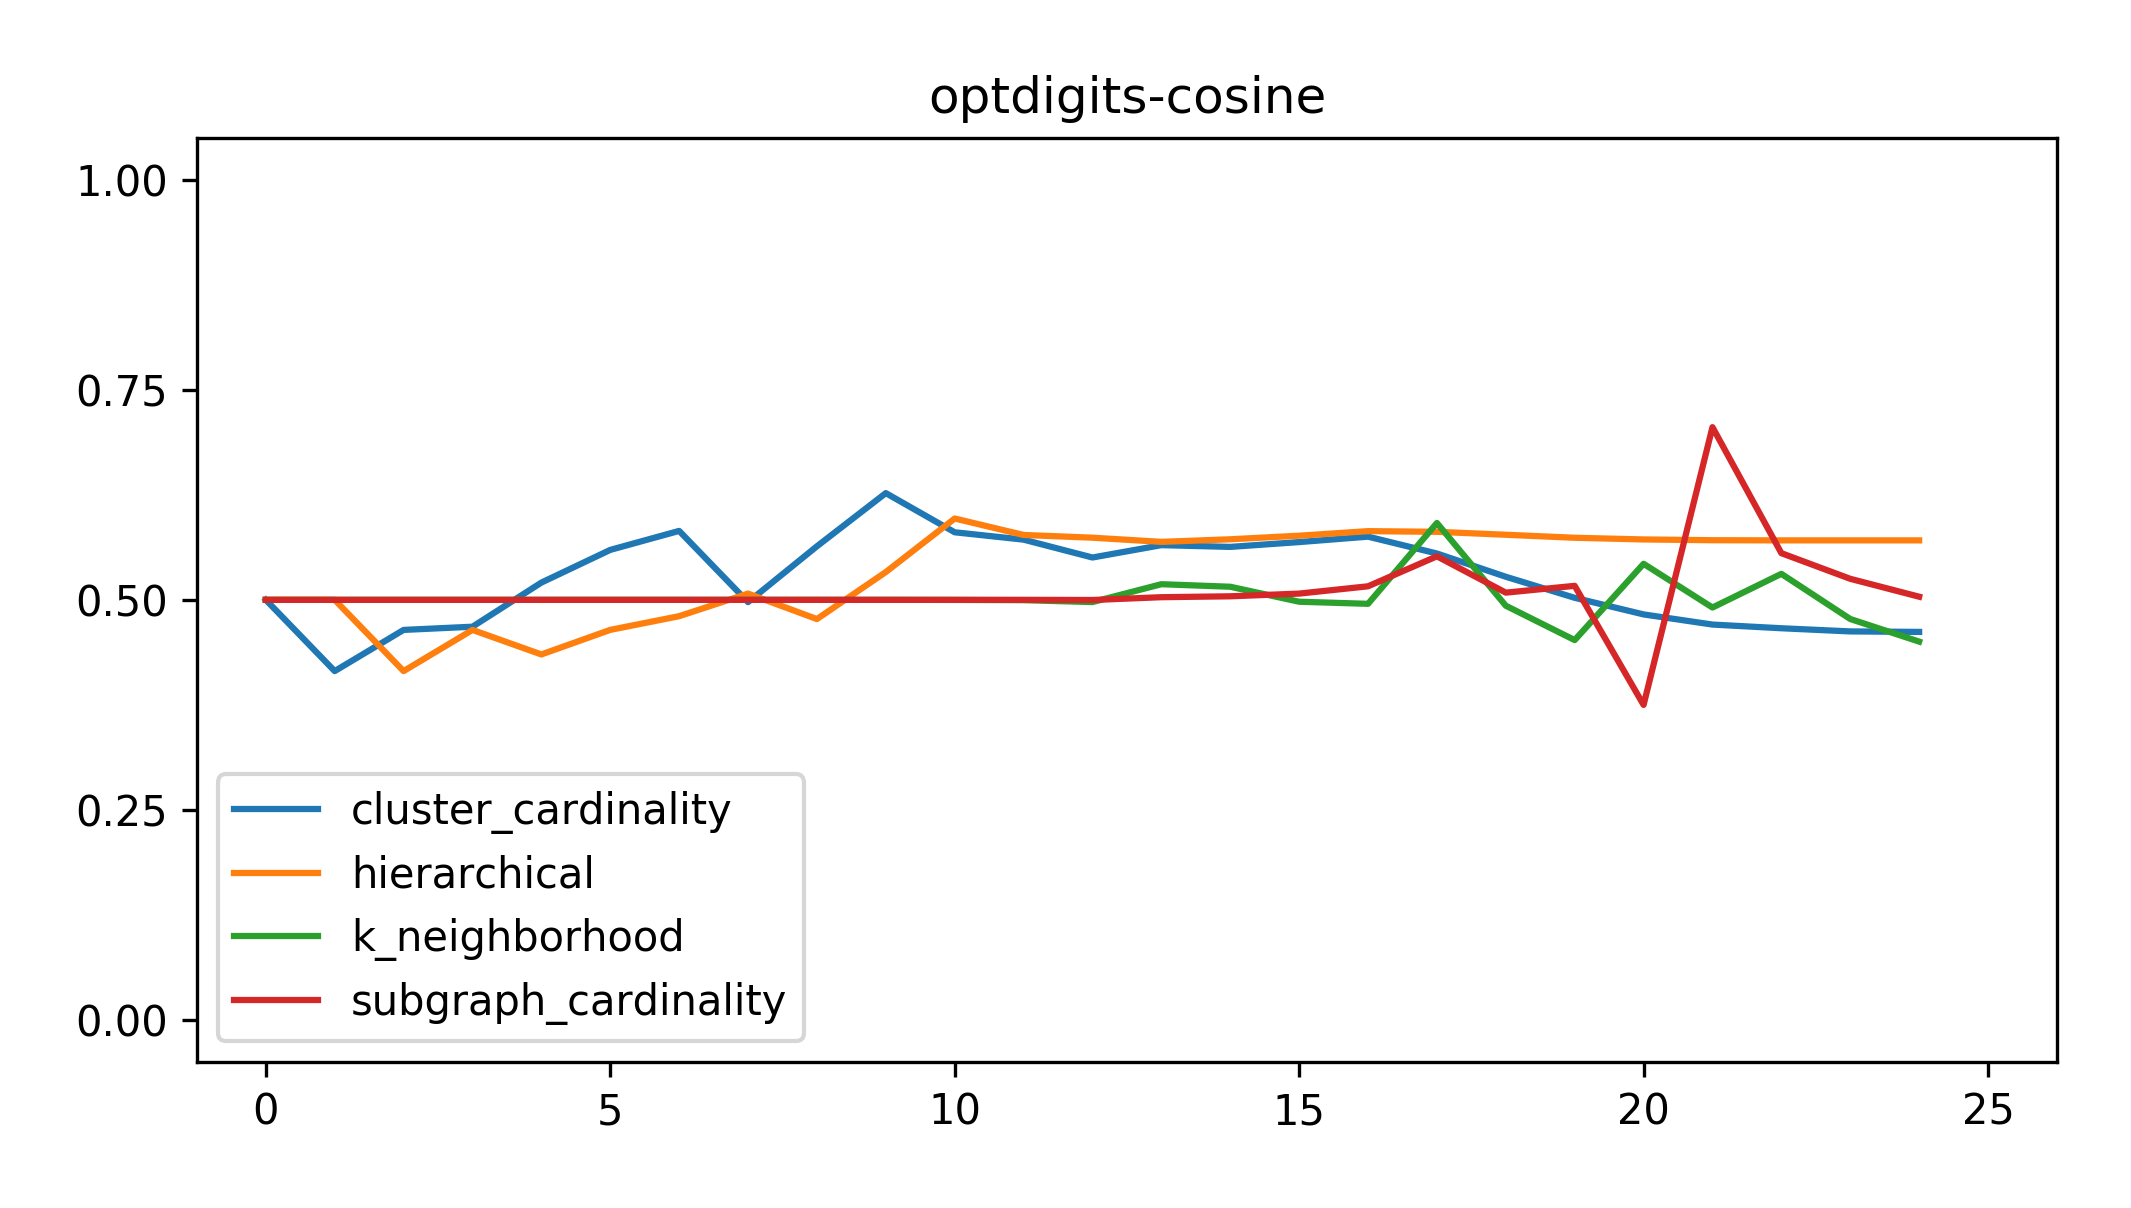
\includegraphics[width=2.2in]{kdd/static/auc_vs_depth/optdigits-cosine.png}
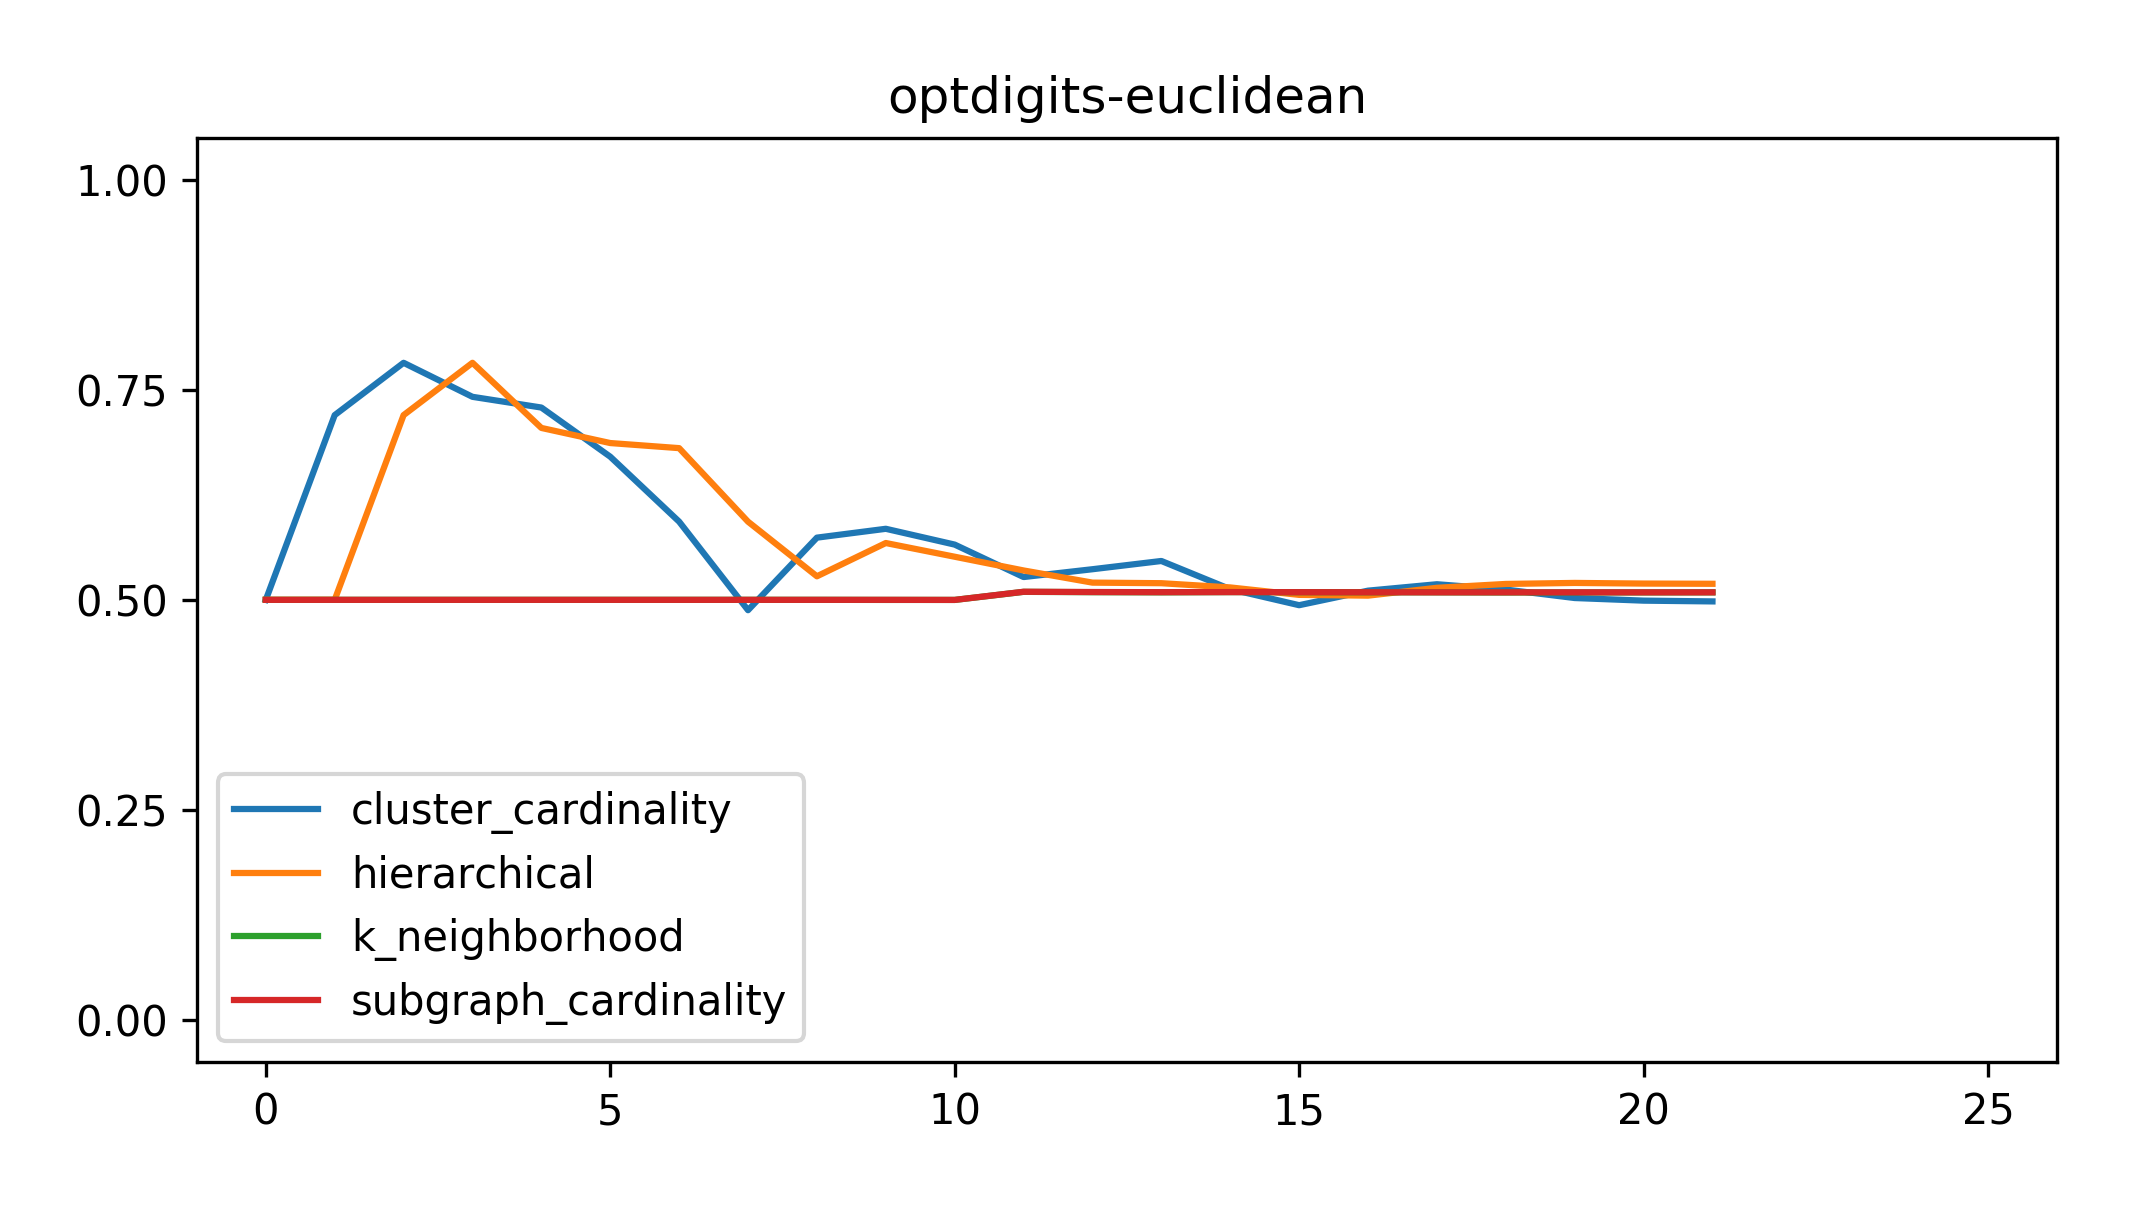
\includegraphics[width=2.2in]{kdd/static/auc_vs_depth/optdigits-euclidean.png}
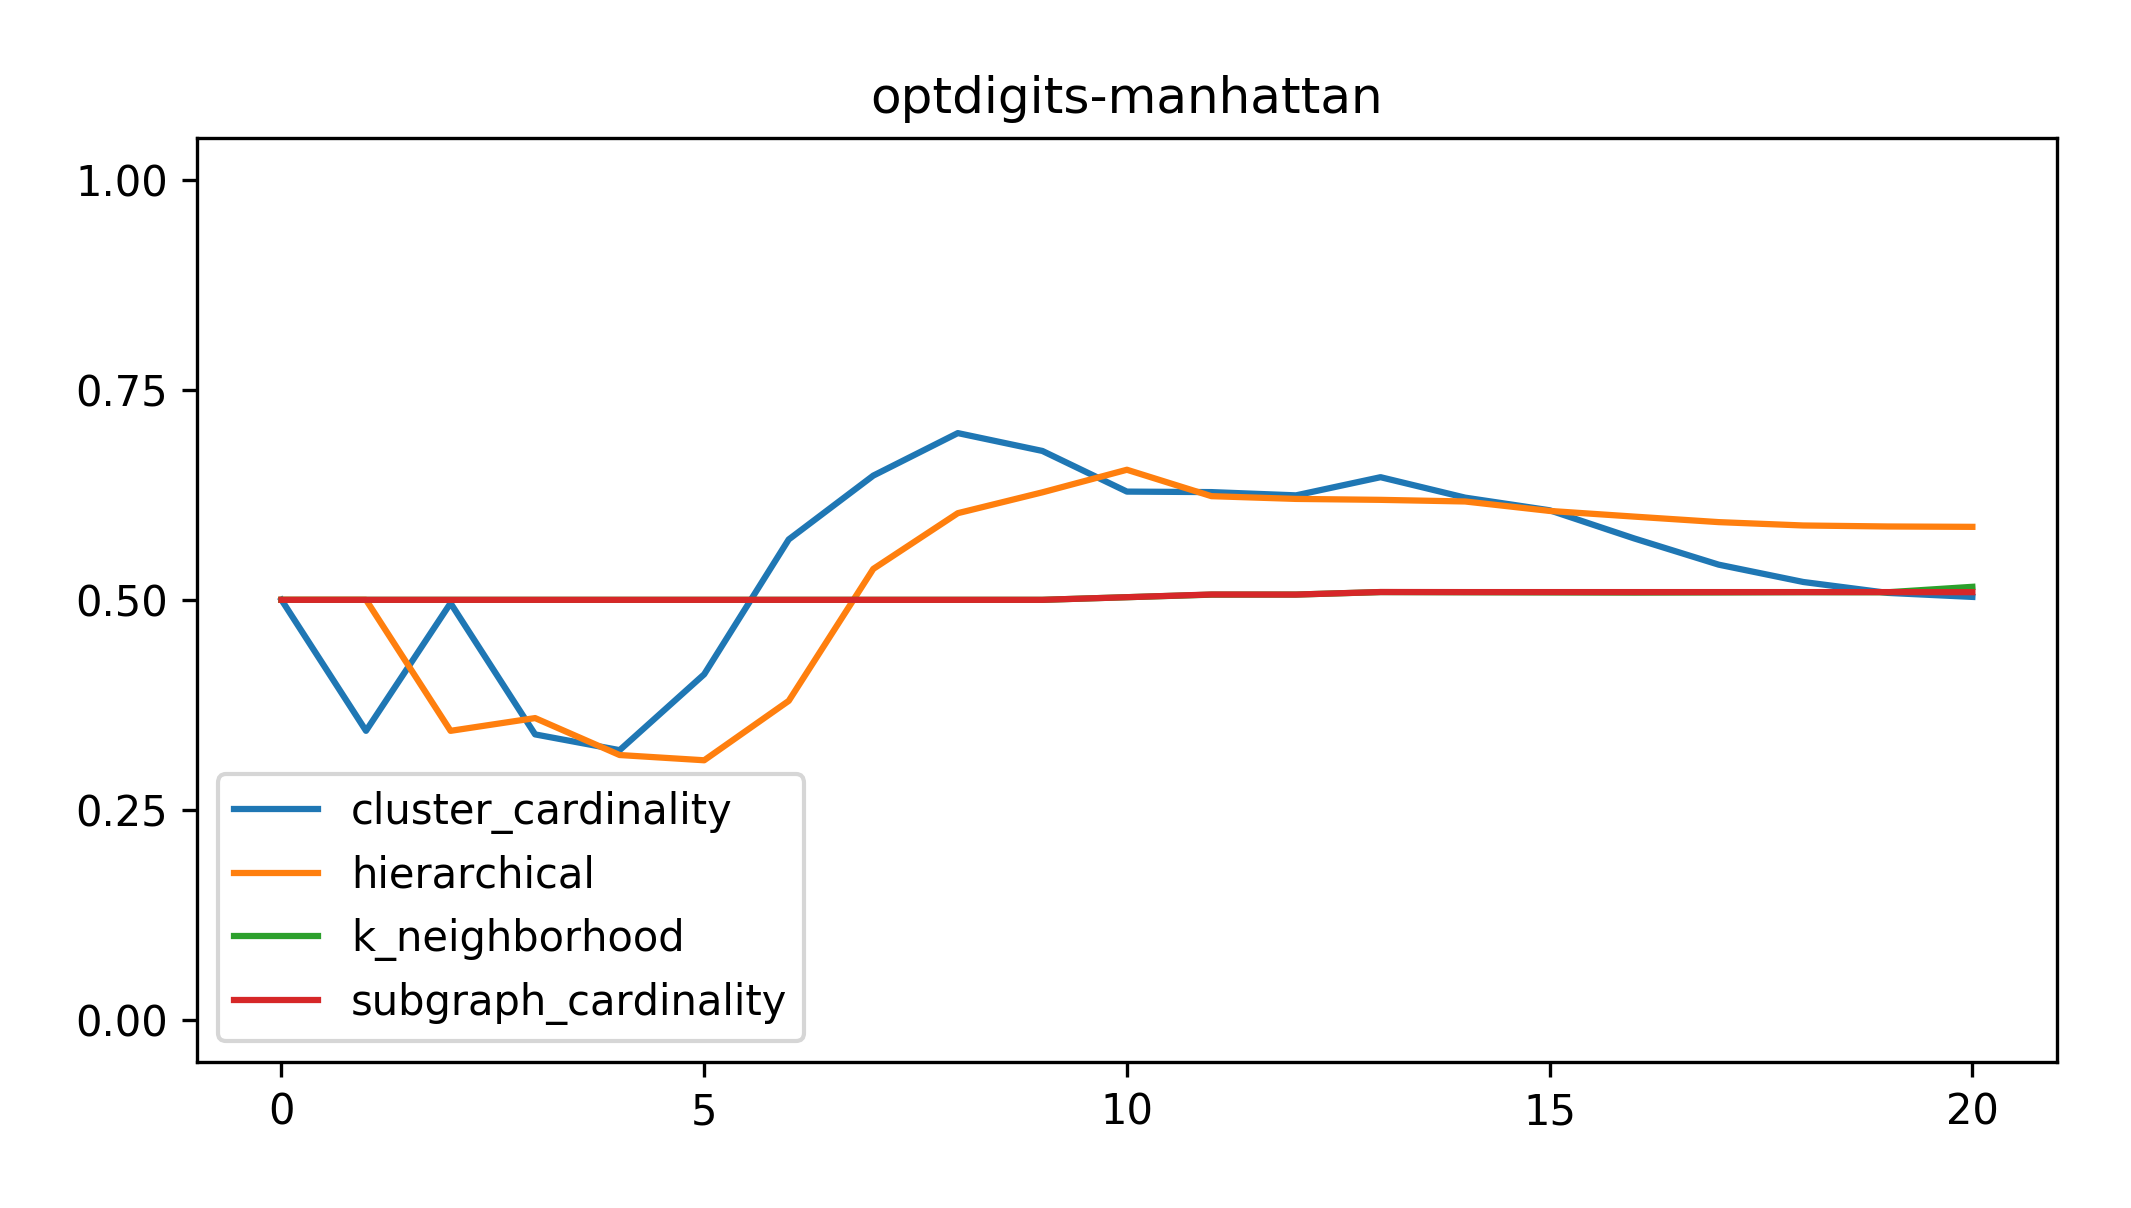
\includegraphics[width=2.2in]{kdd/static/auc_vs_depth/optdigits-manhattan.png}

% Pima
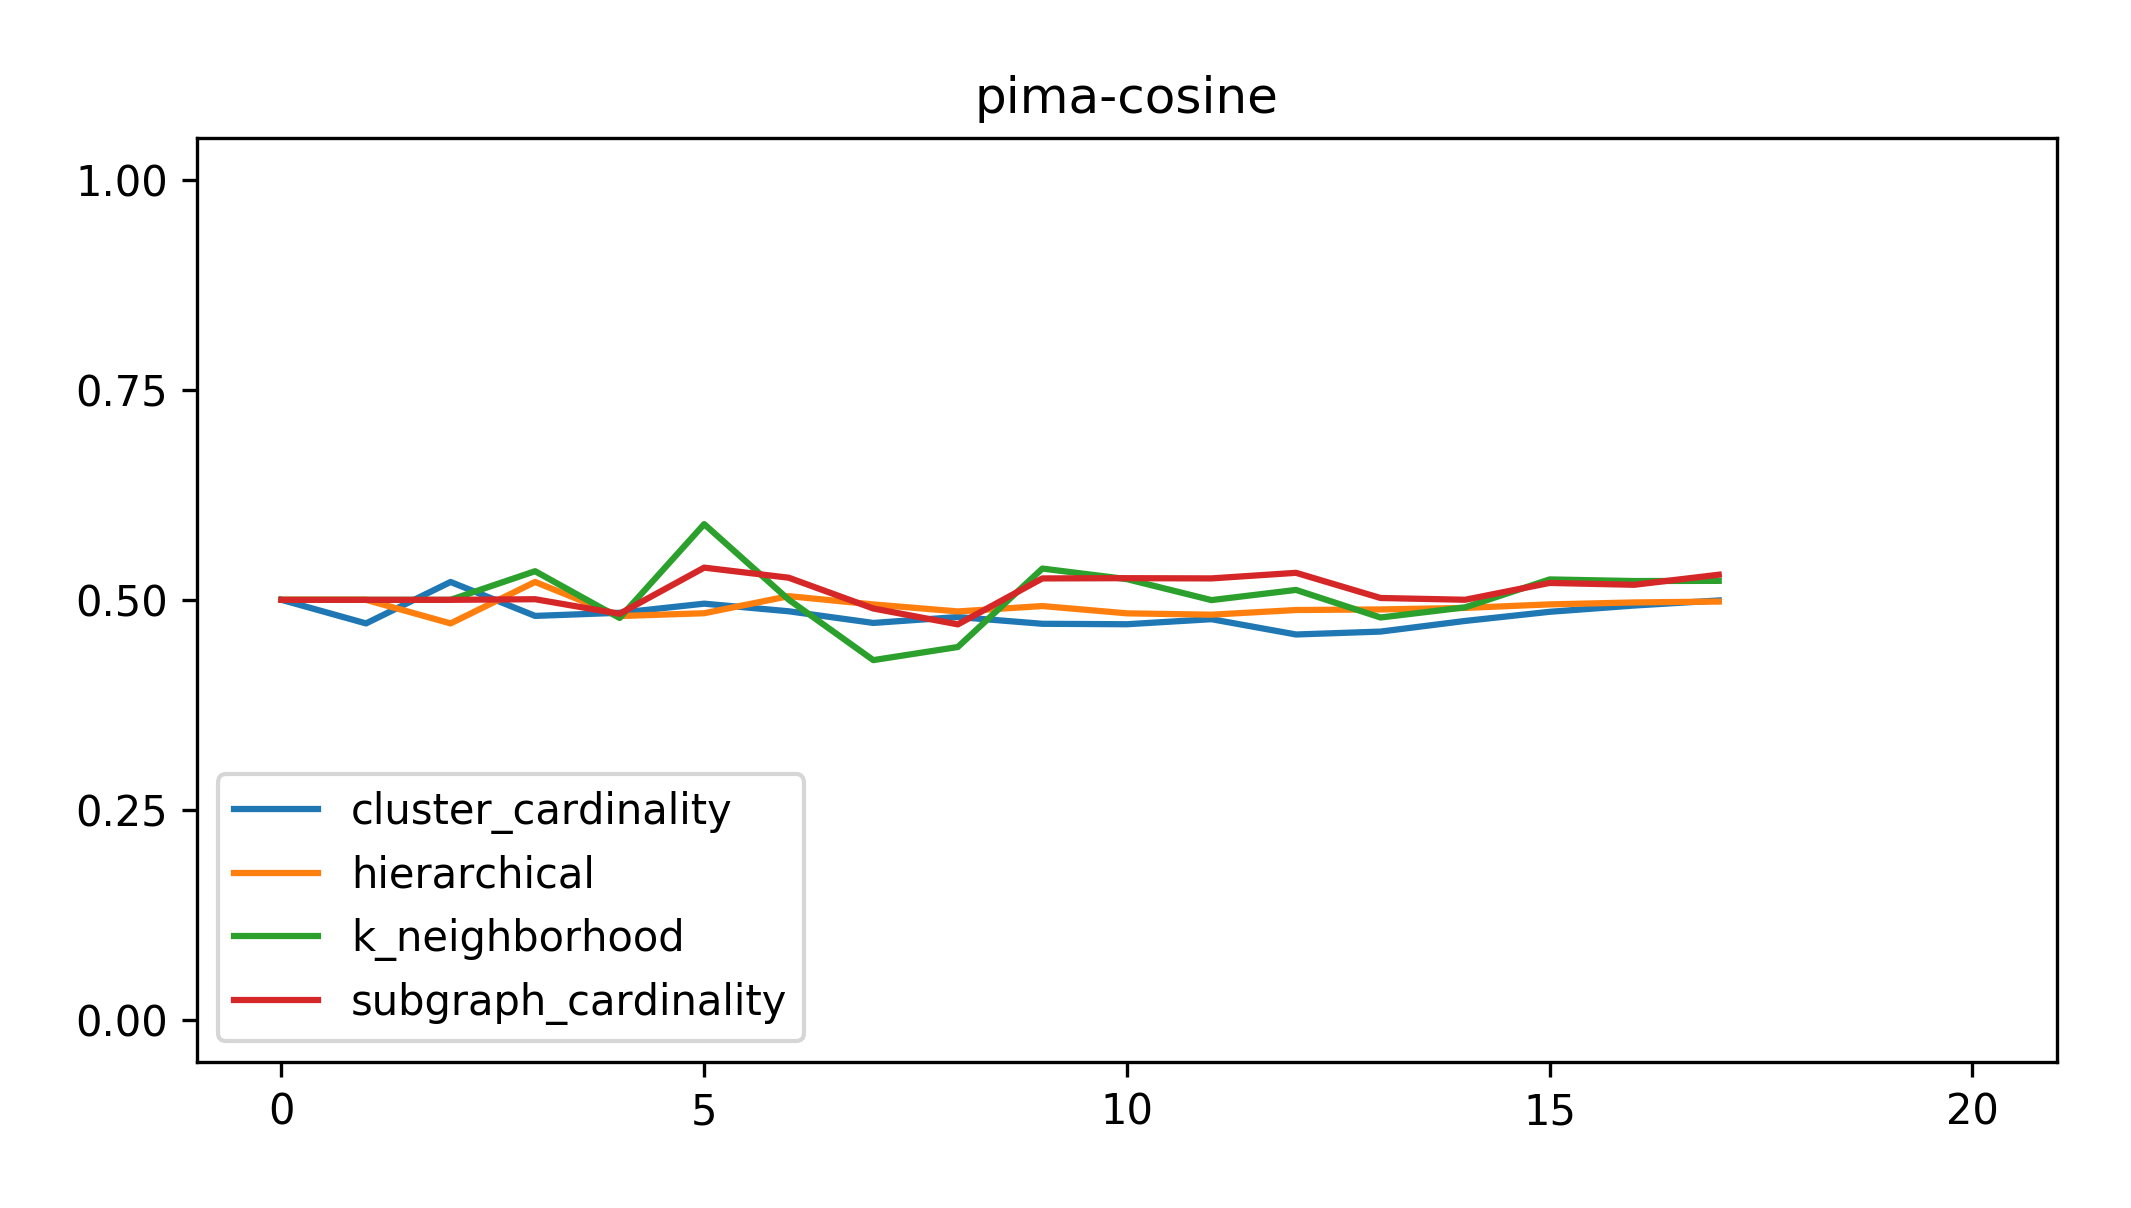
\includegraphics[width=2.2in]{kdd/static/auc_vs_depth/pima-cosine.png}
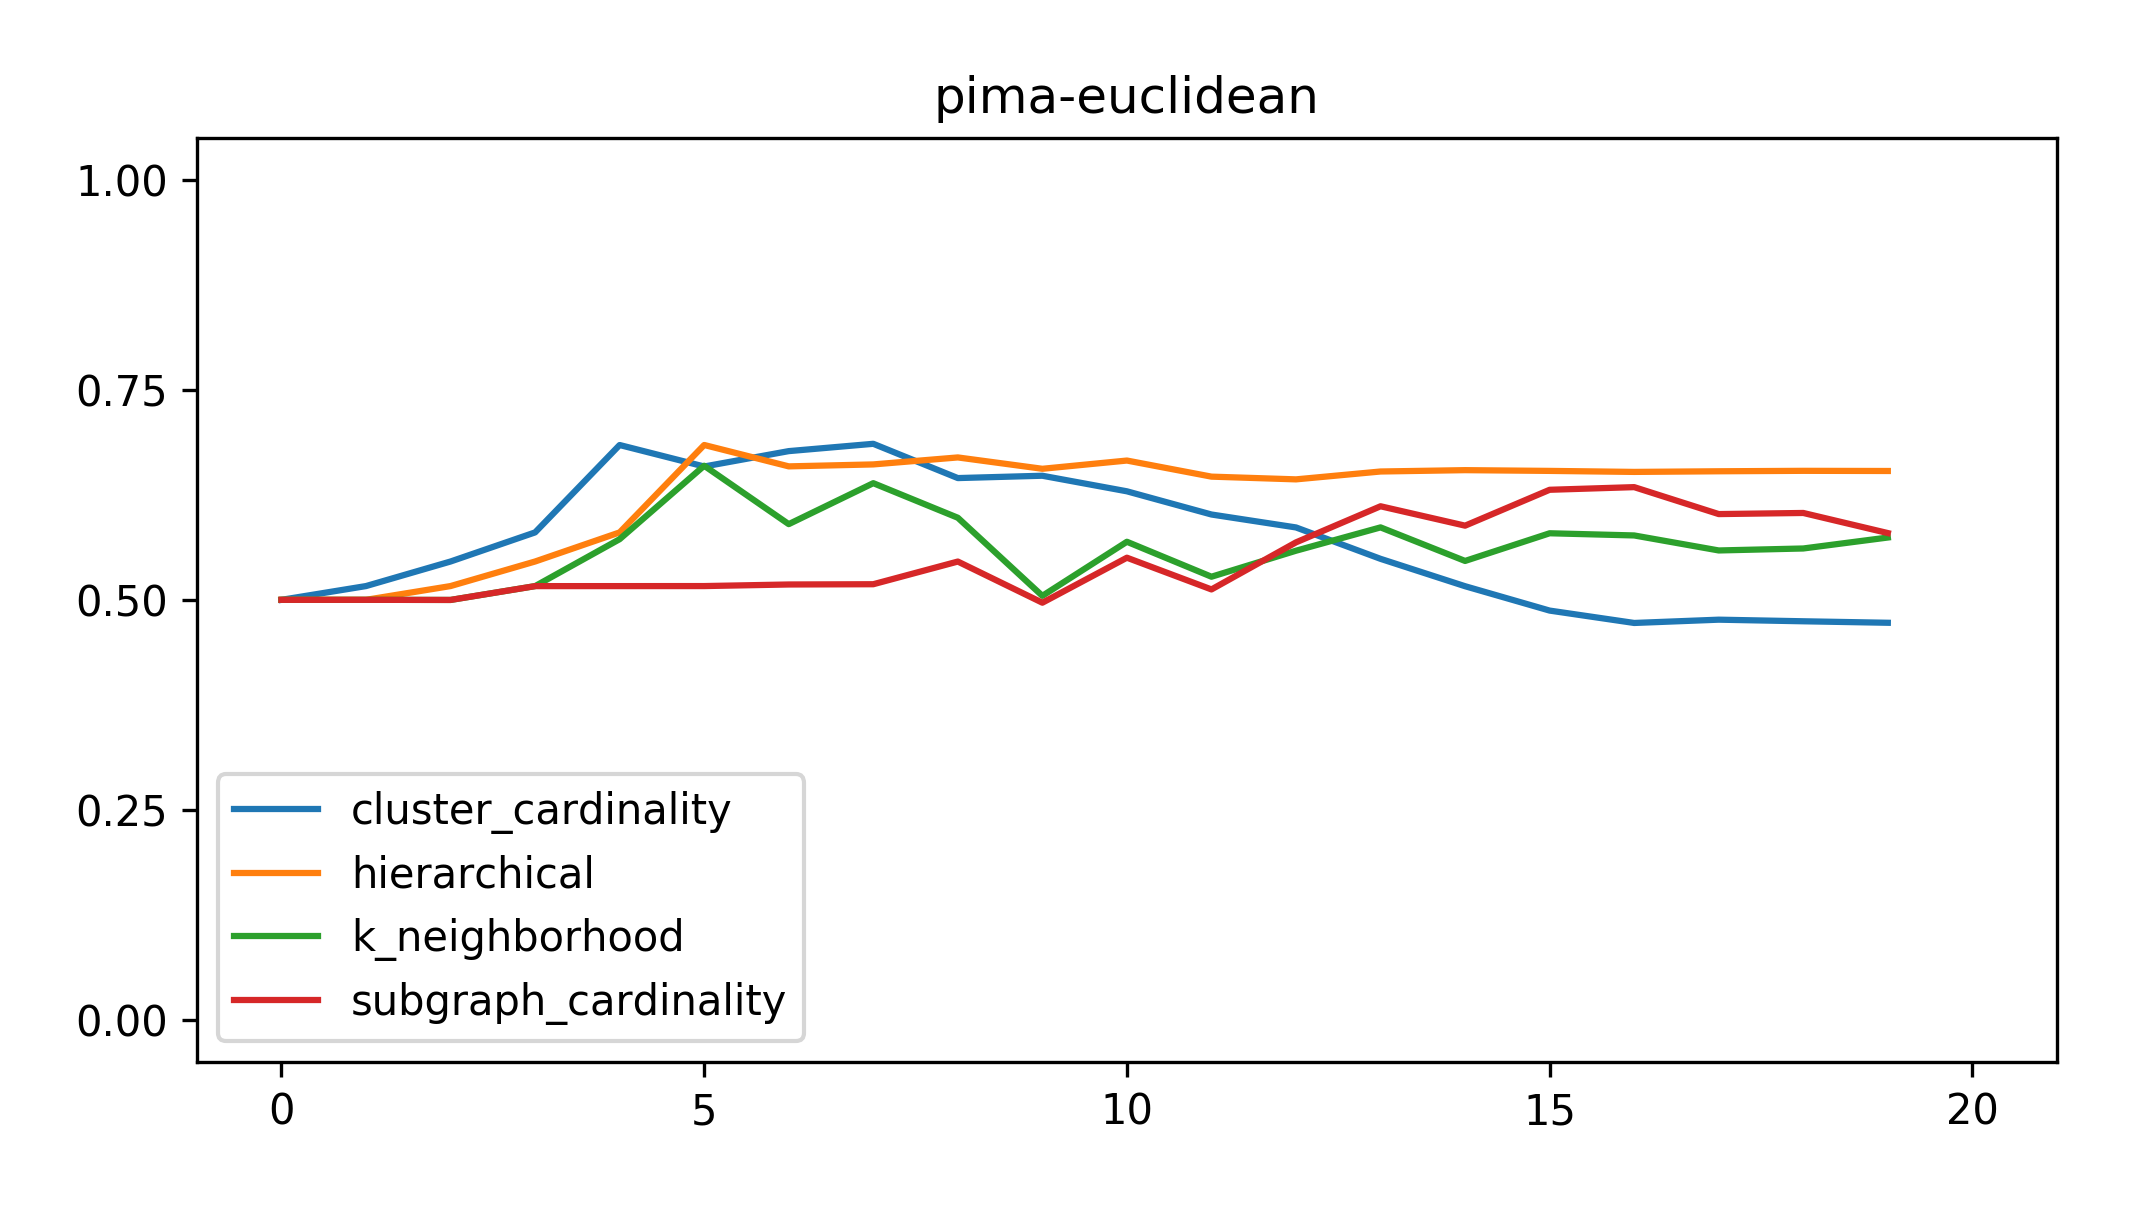
\includegraphics[width=2.2in]{kdd/static/auc_vs_depth/pima-euclidean.png}
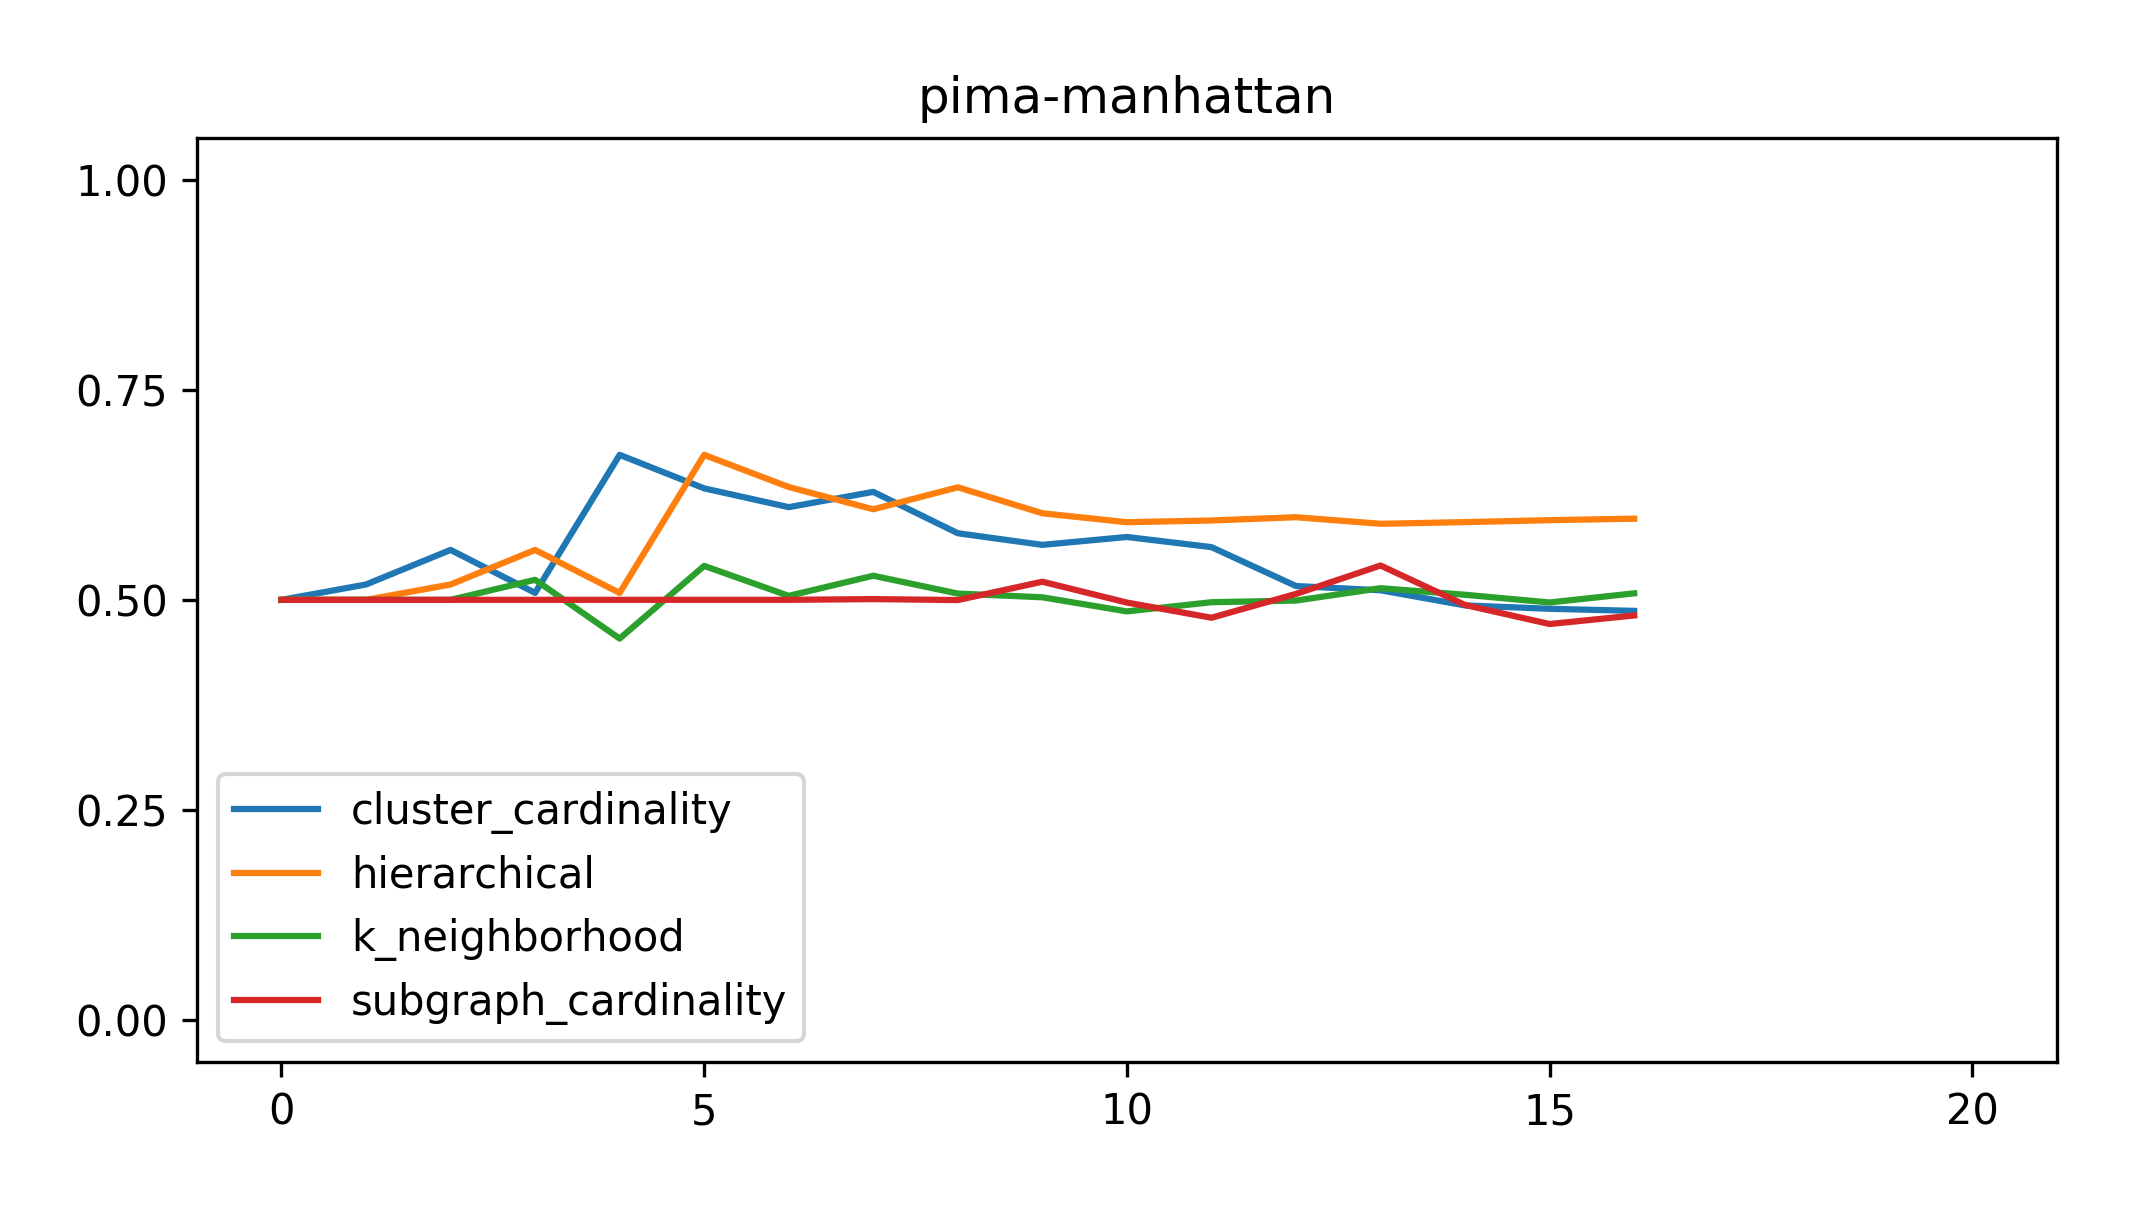
\includegraphics[width=2.2in]{kdd/static/auc_vs_depth/pima-manhattan.png}

% Satellite
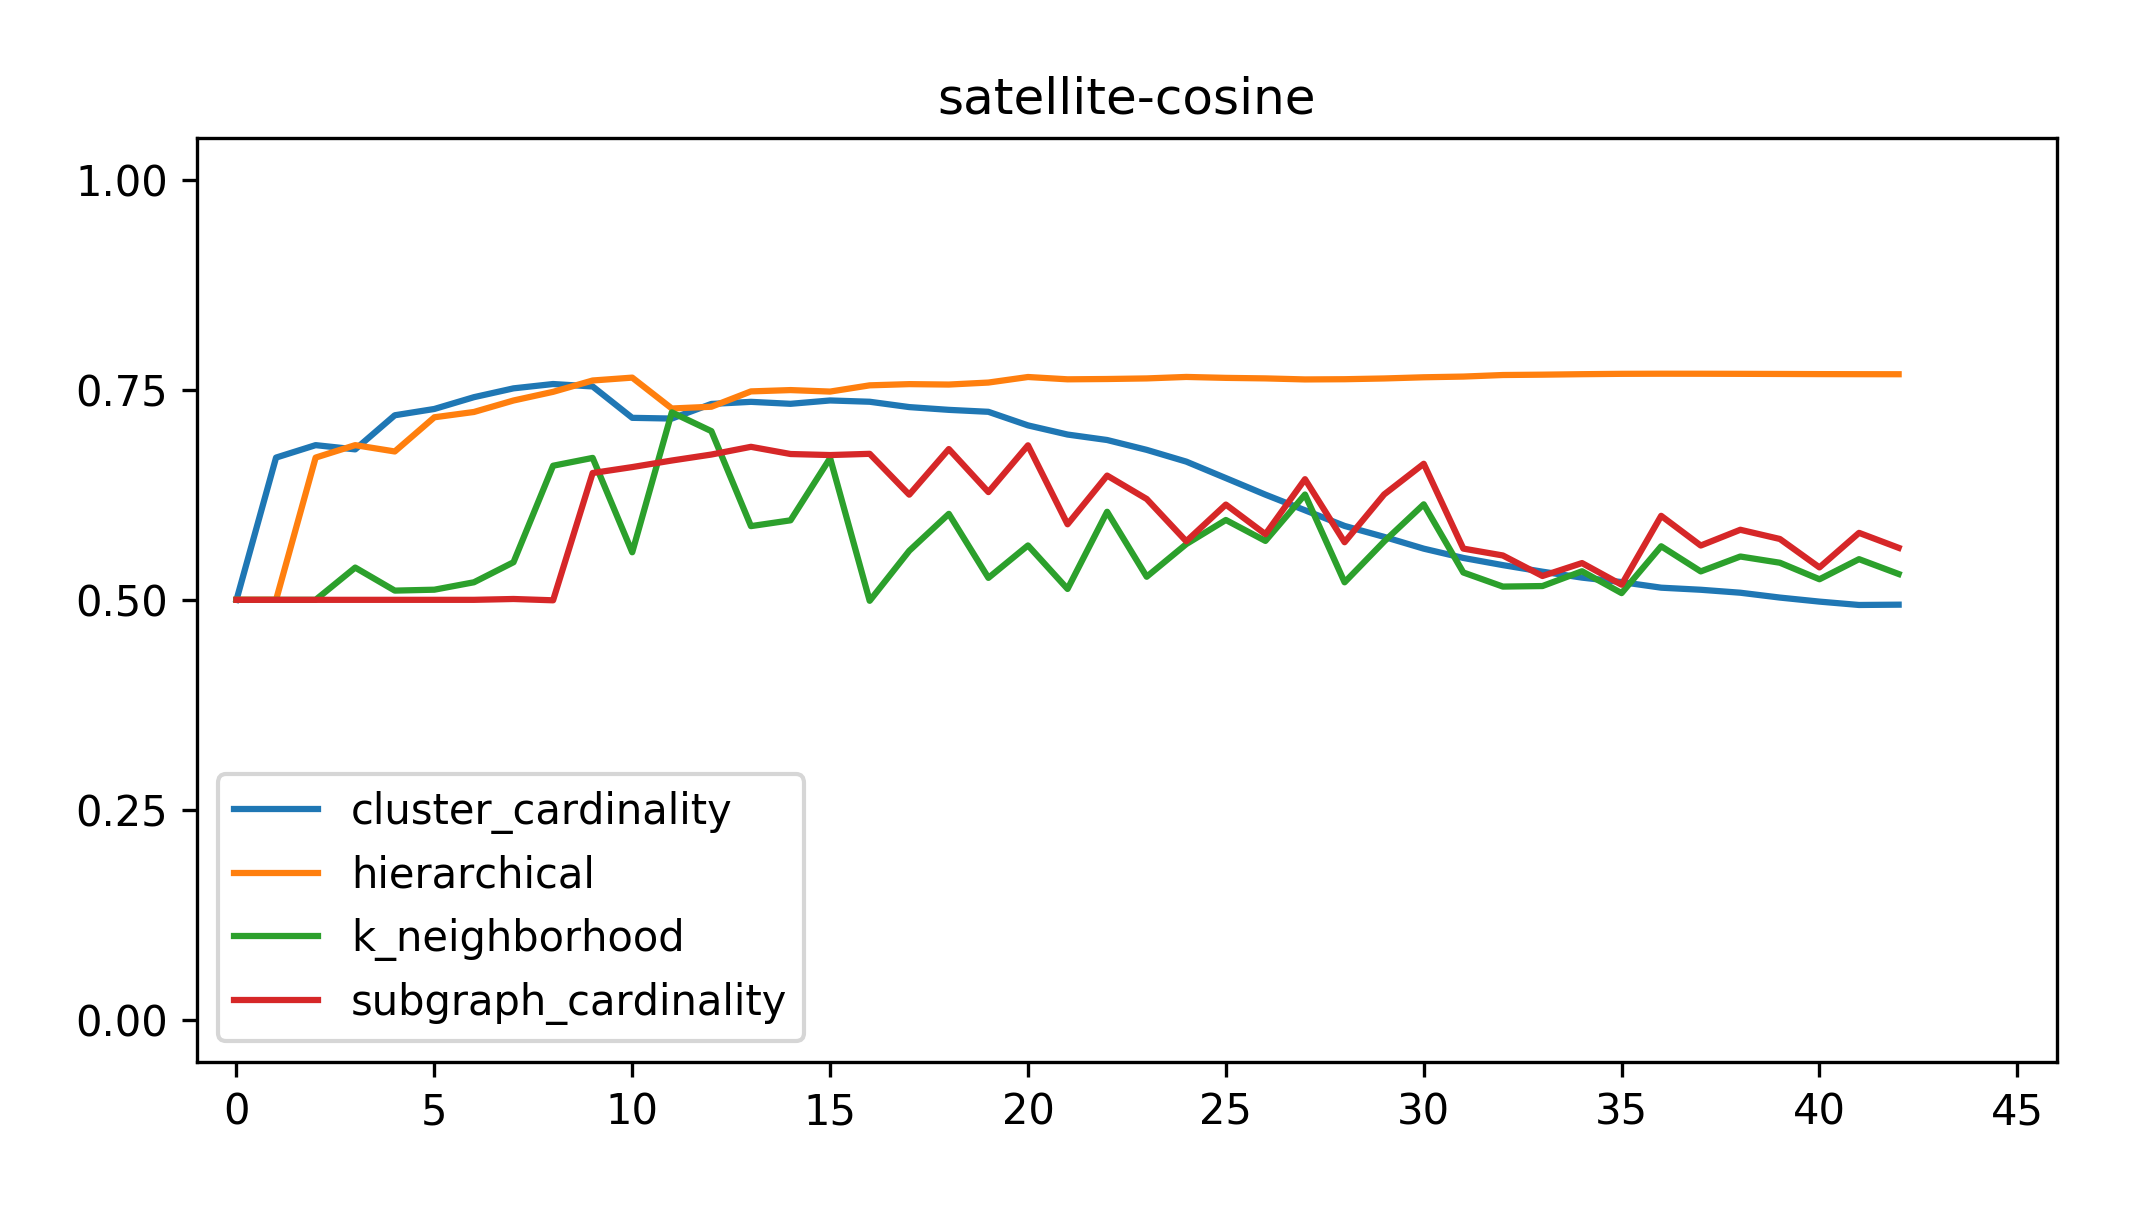
\includegraphics[width=2.2in]{kdd/static/auc_vs_depth/satellite-cosine.png}
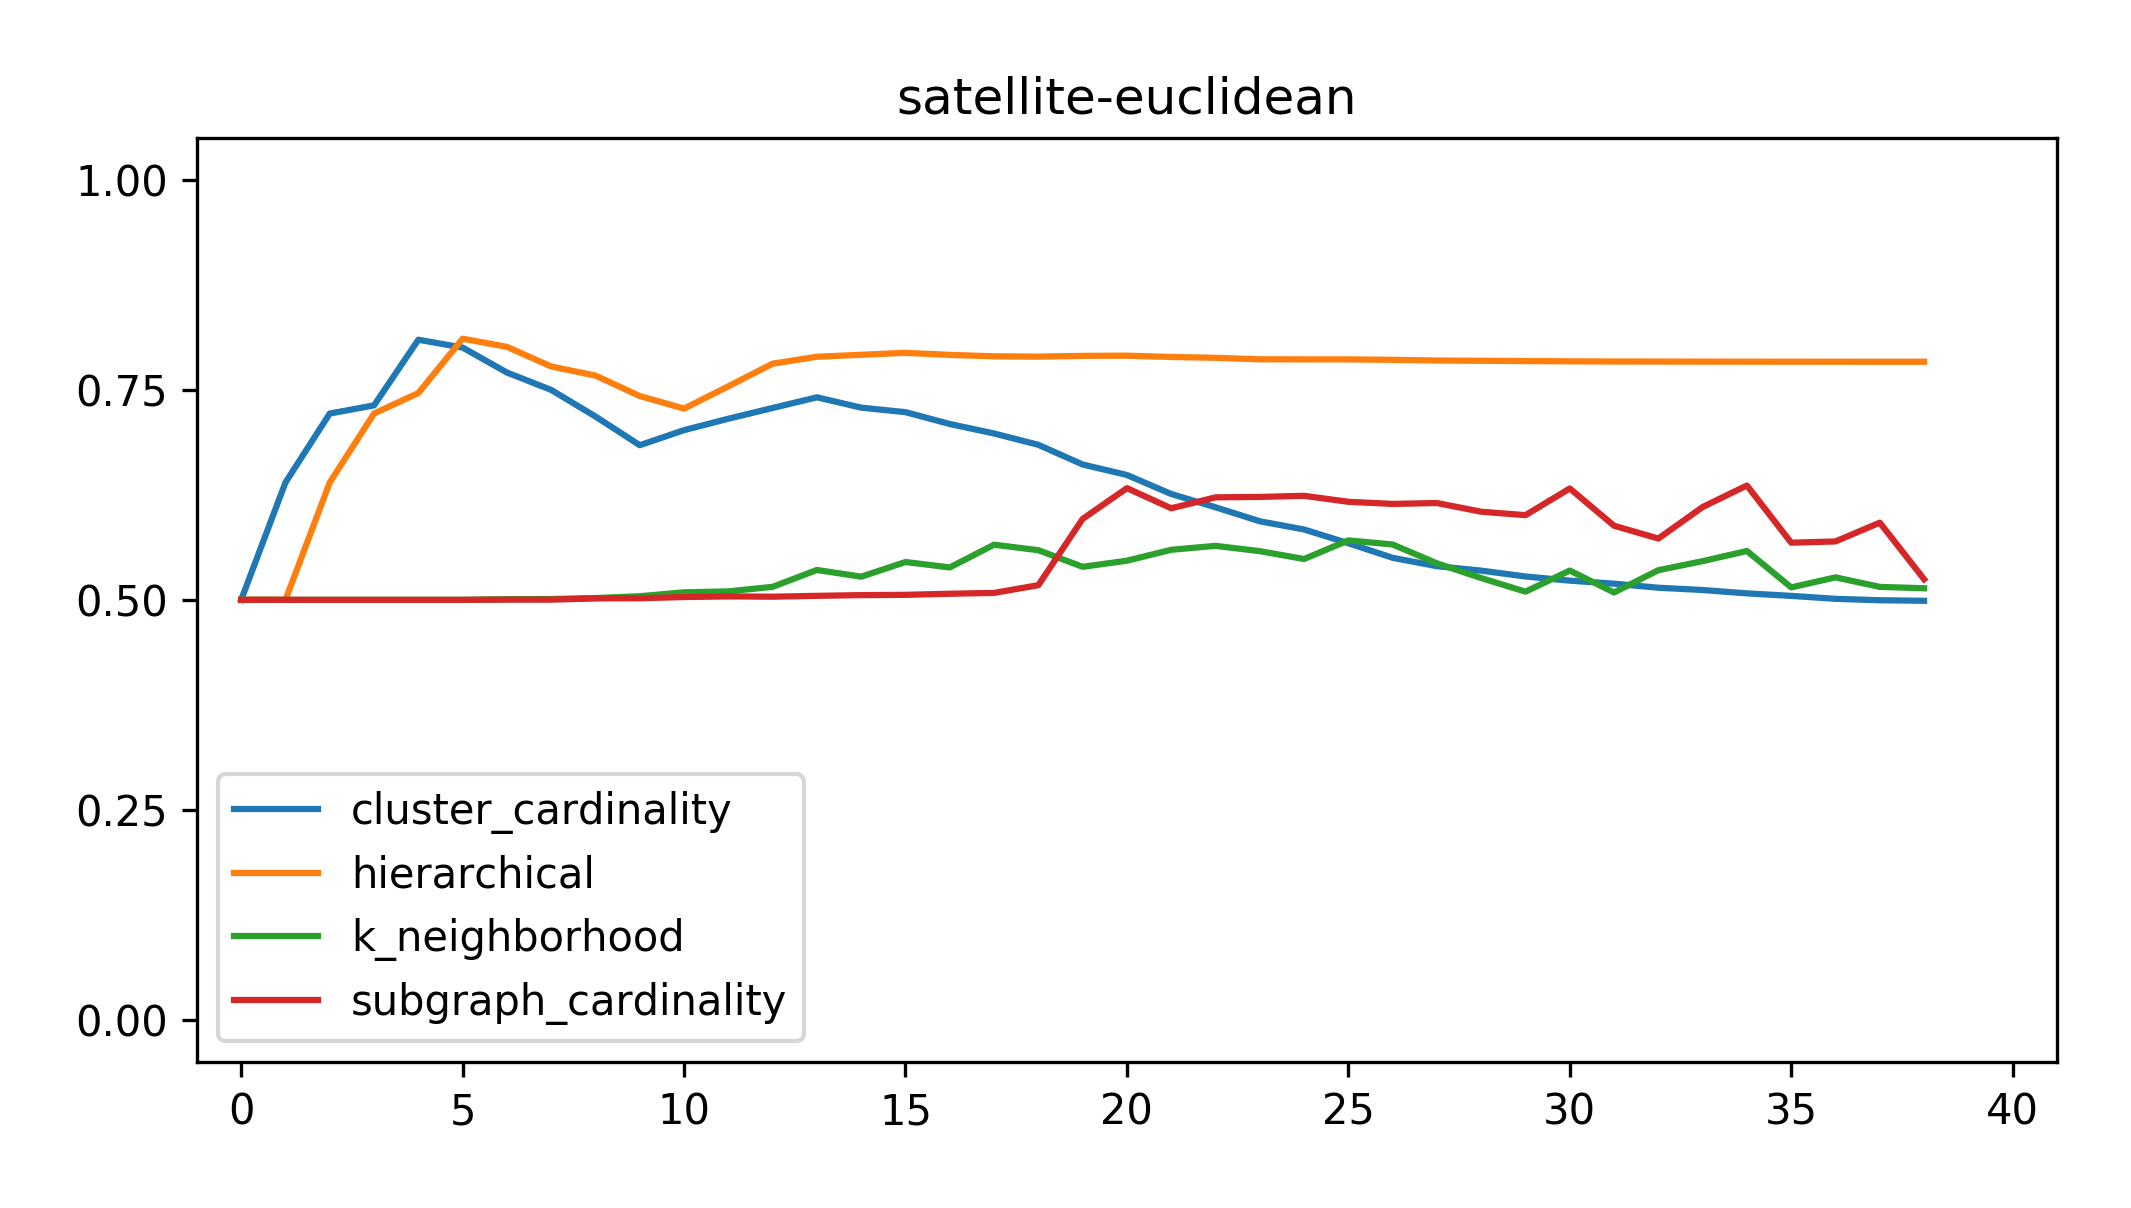
\includegraphics[width=2.2in]{kdd/static/auc_vs_depth/satellite-euclidean.png}
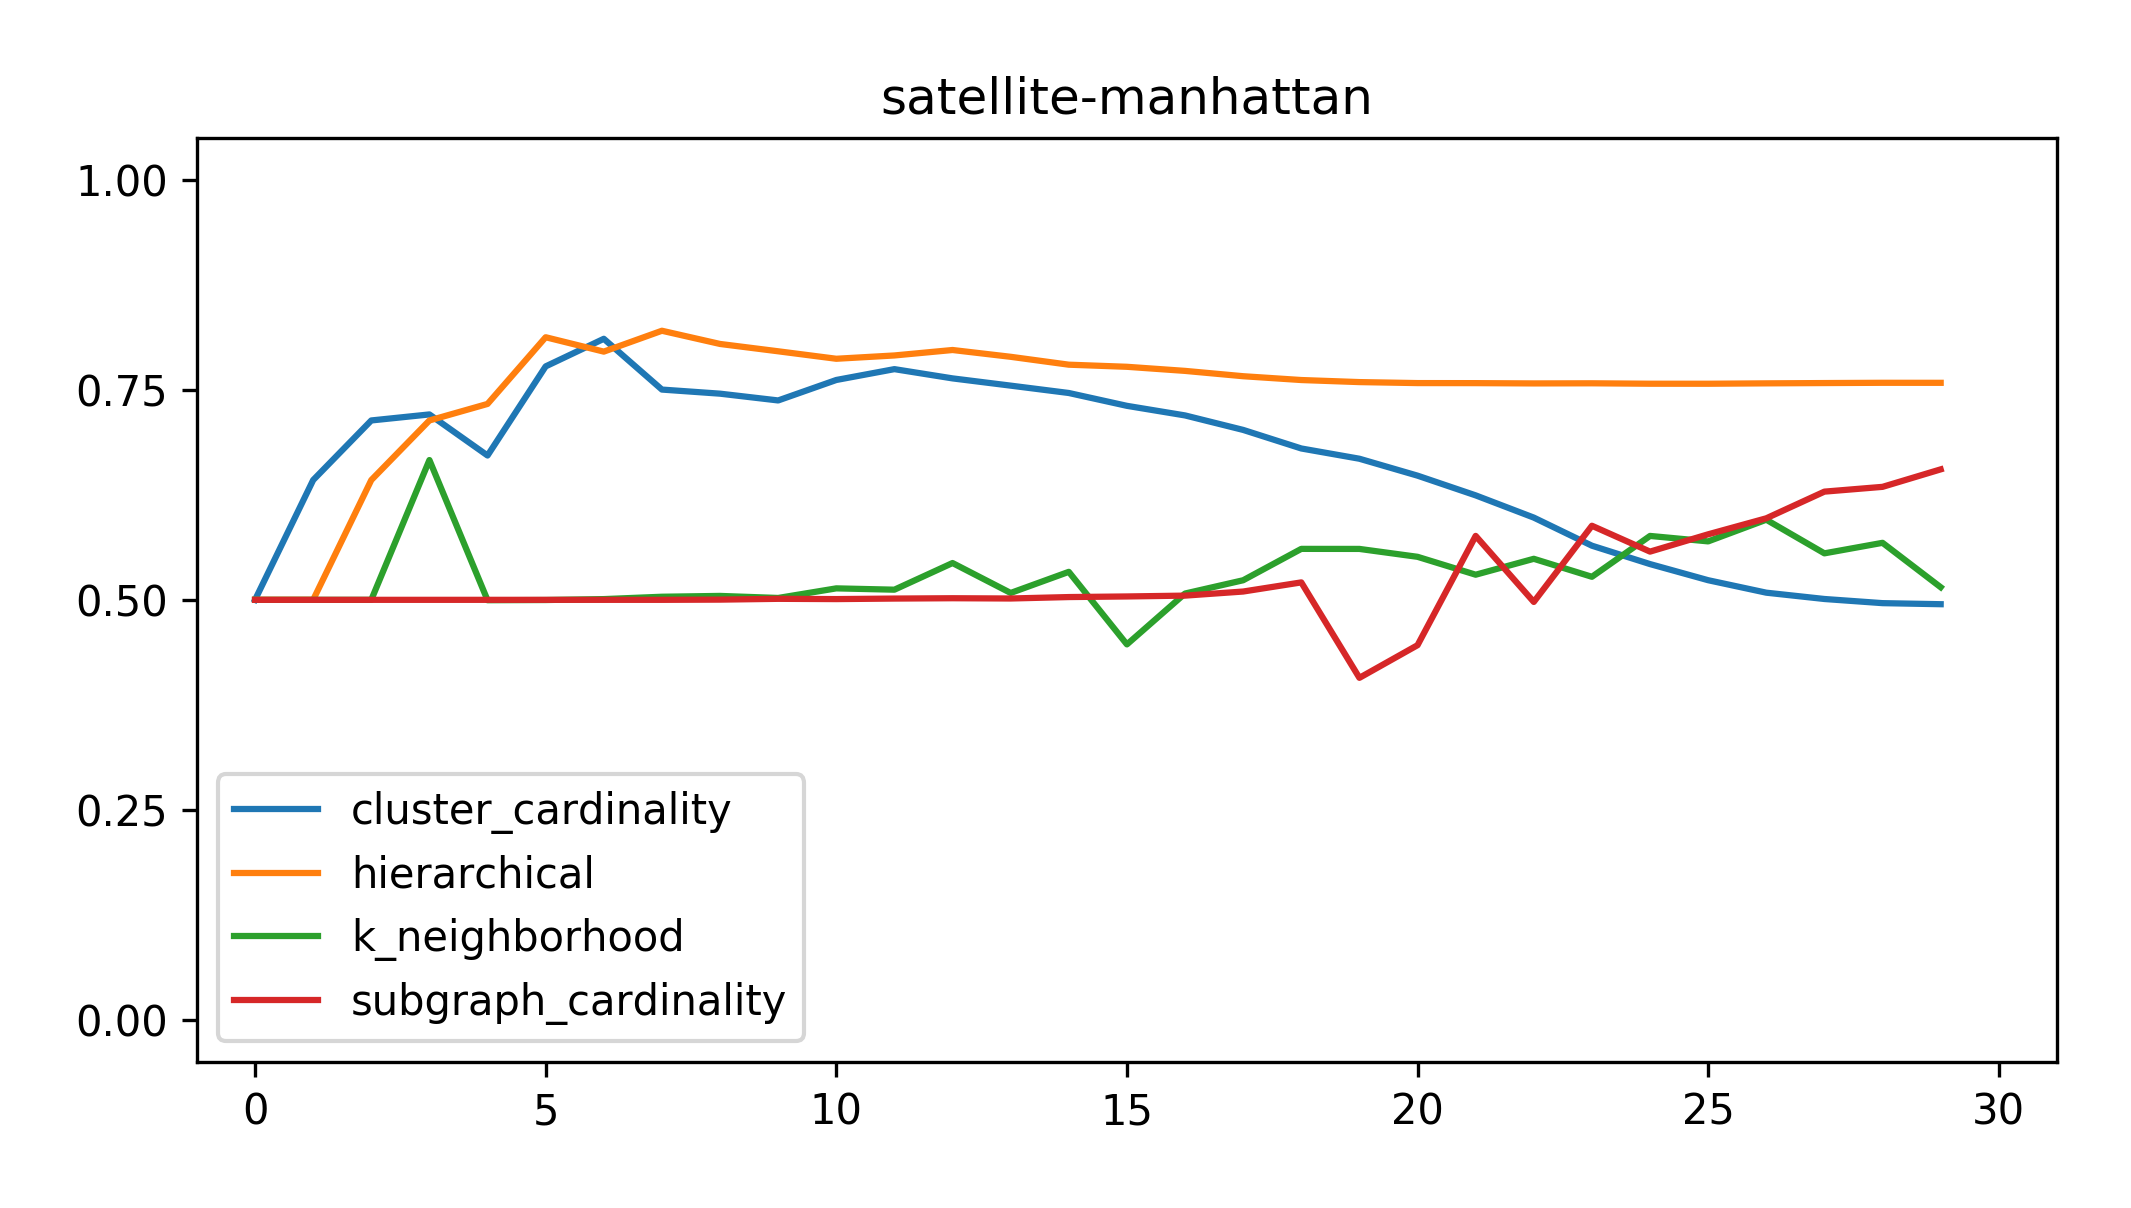
\includegraphics[width=2.2in]{kdd/static/auc_vs_depth/satellite-manhattan.png}

\caption{
Plots of ROC-AUC vs Depth for our mearures of Anomolousness.
}

\label{results:datasets_2}
\end{figure*}

\begin{figure*}[!t]
\centering
% Satimage-2
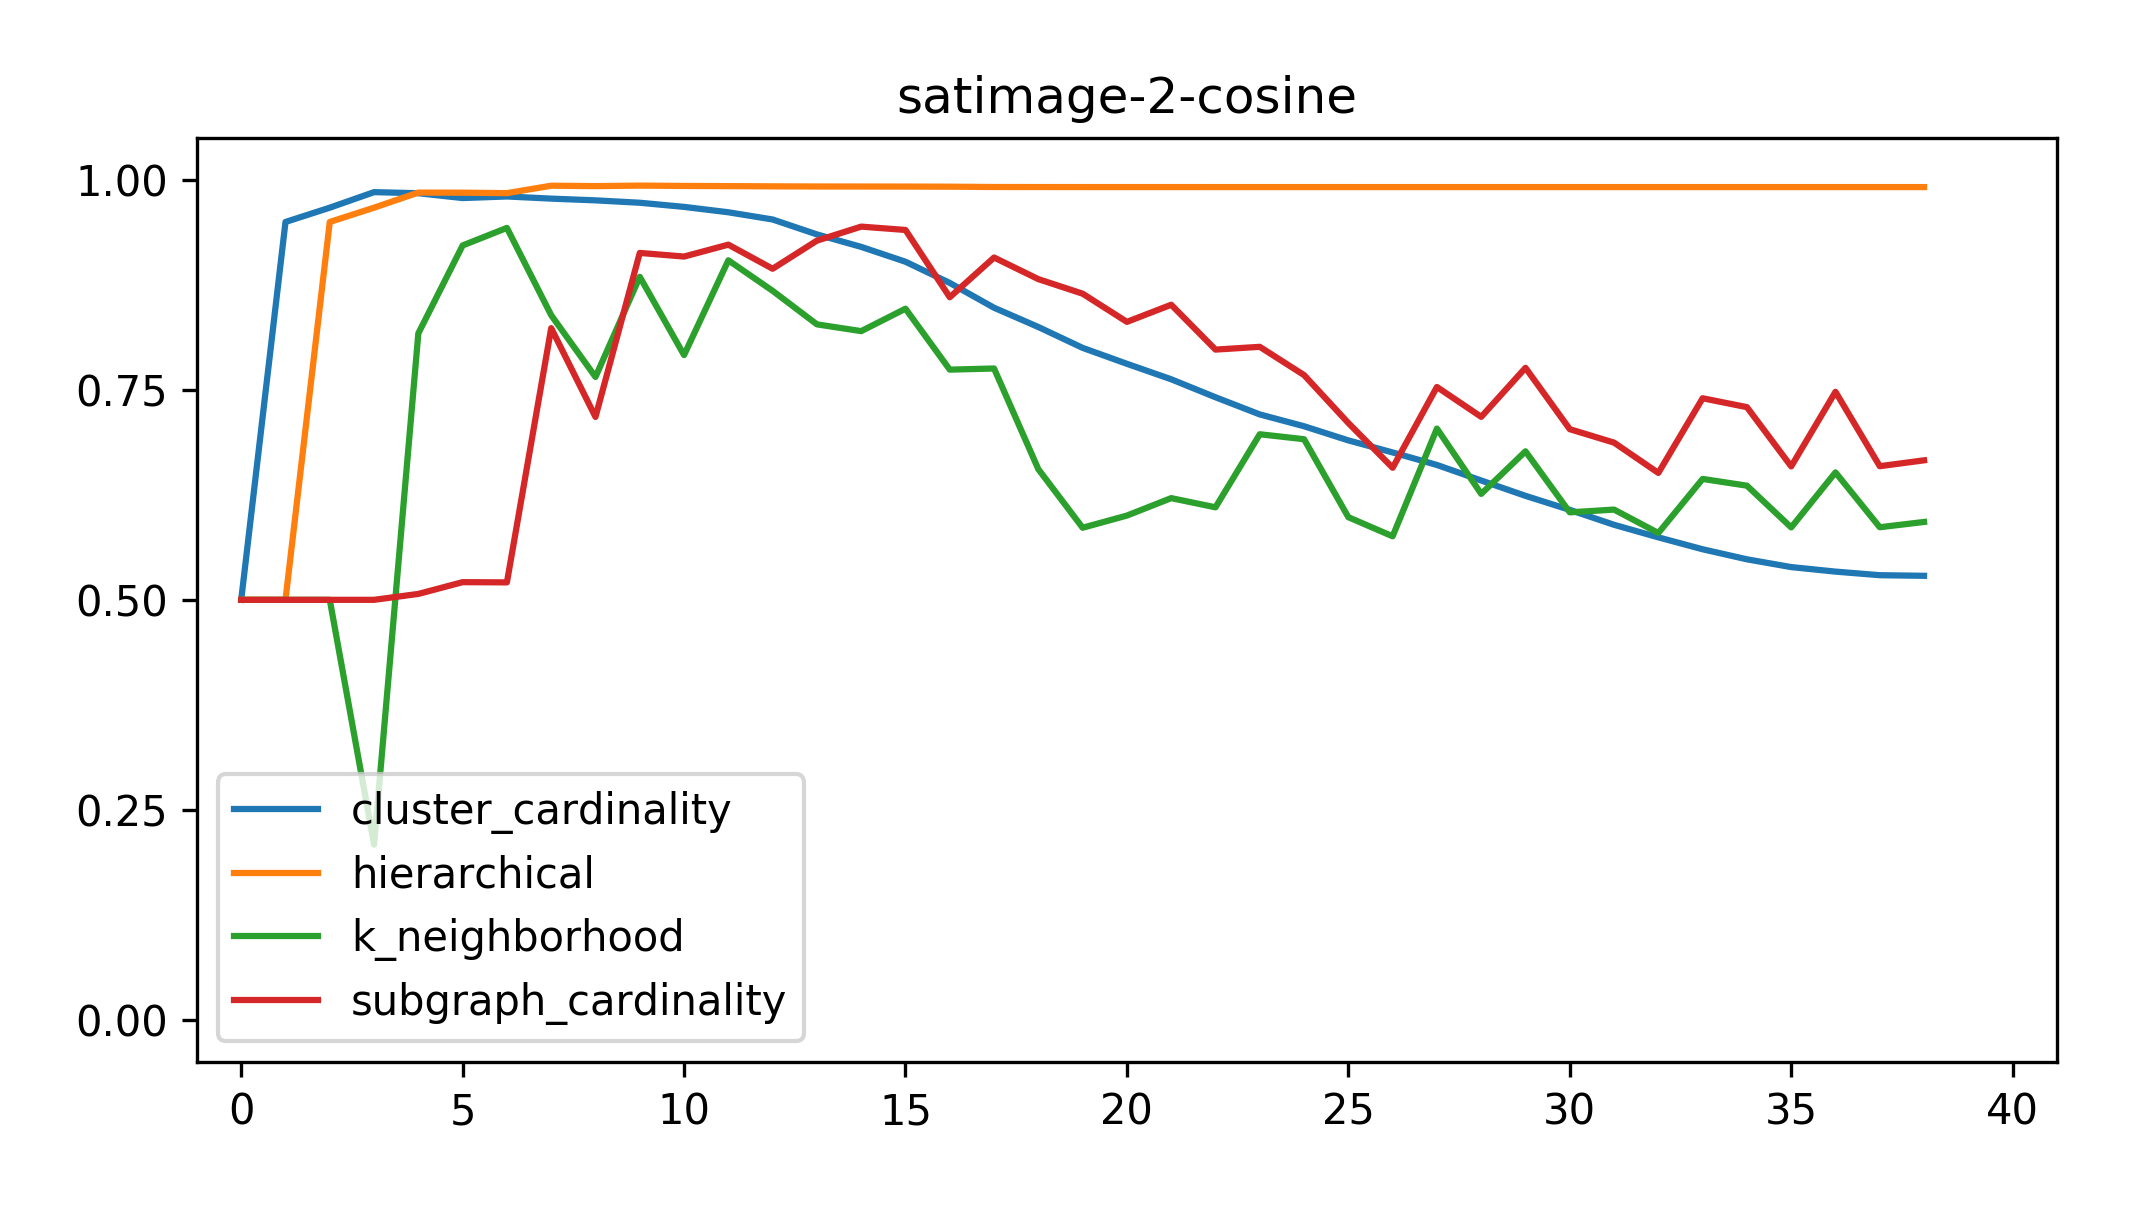
\includegraphics[width=2.2in]{kdd/static/auc_vs_depth/satimage-2-cosine.png}
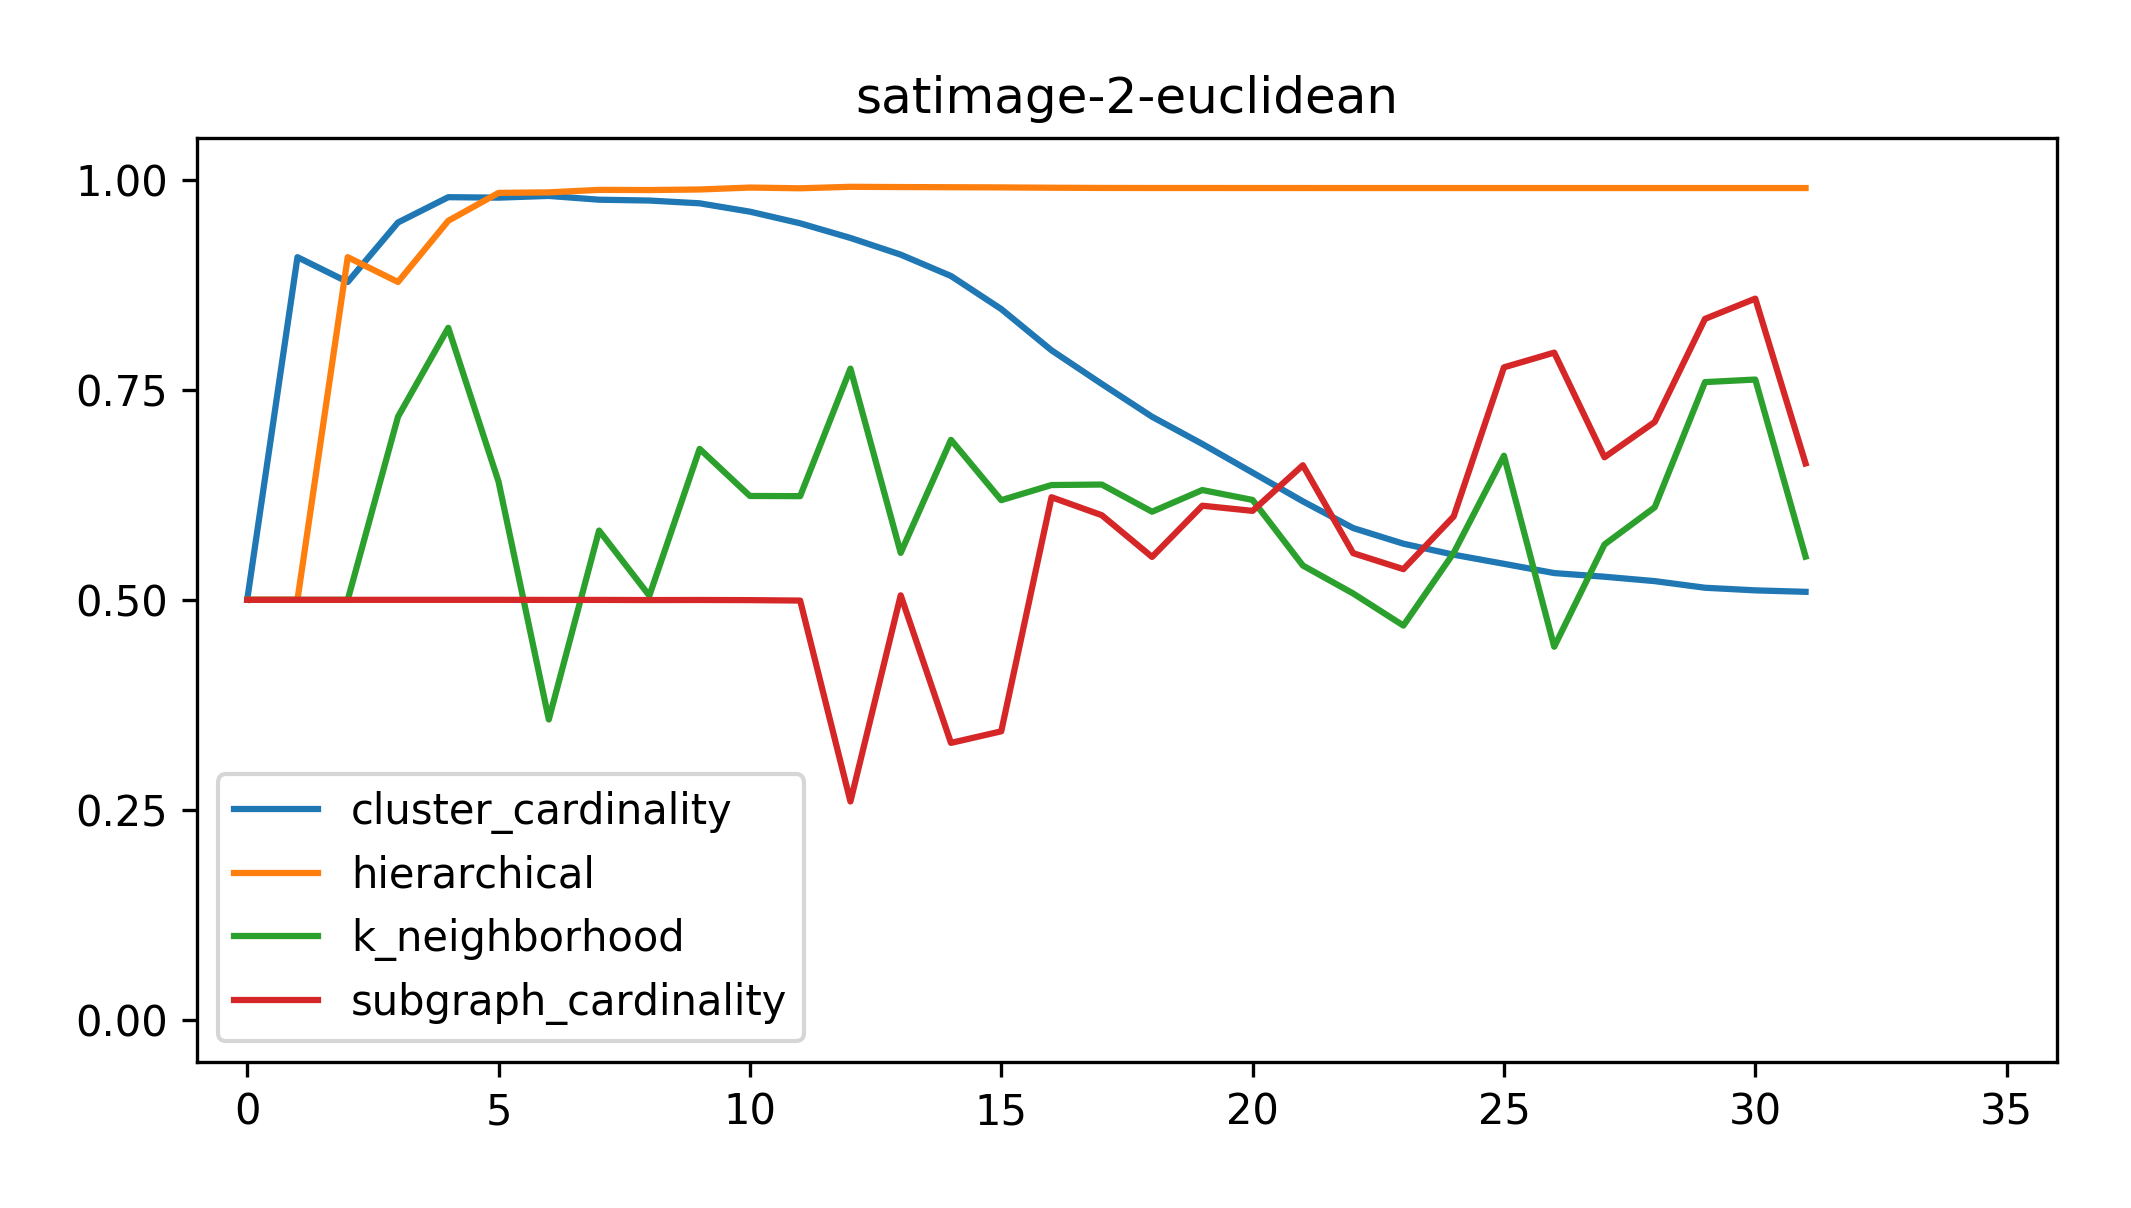
\includegraphics[width=2.2in]{kdd/static/auc_vs_depth/satimage-2-euclidean.png}
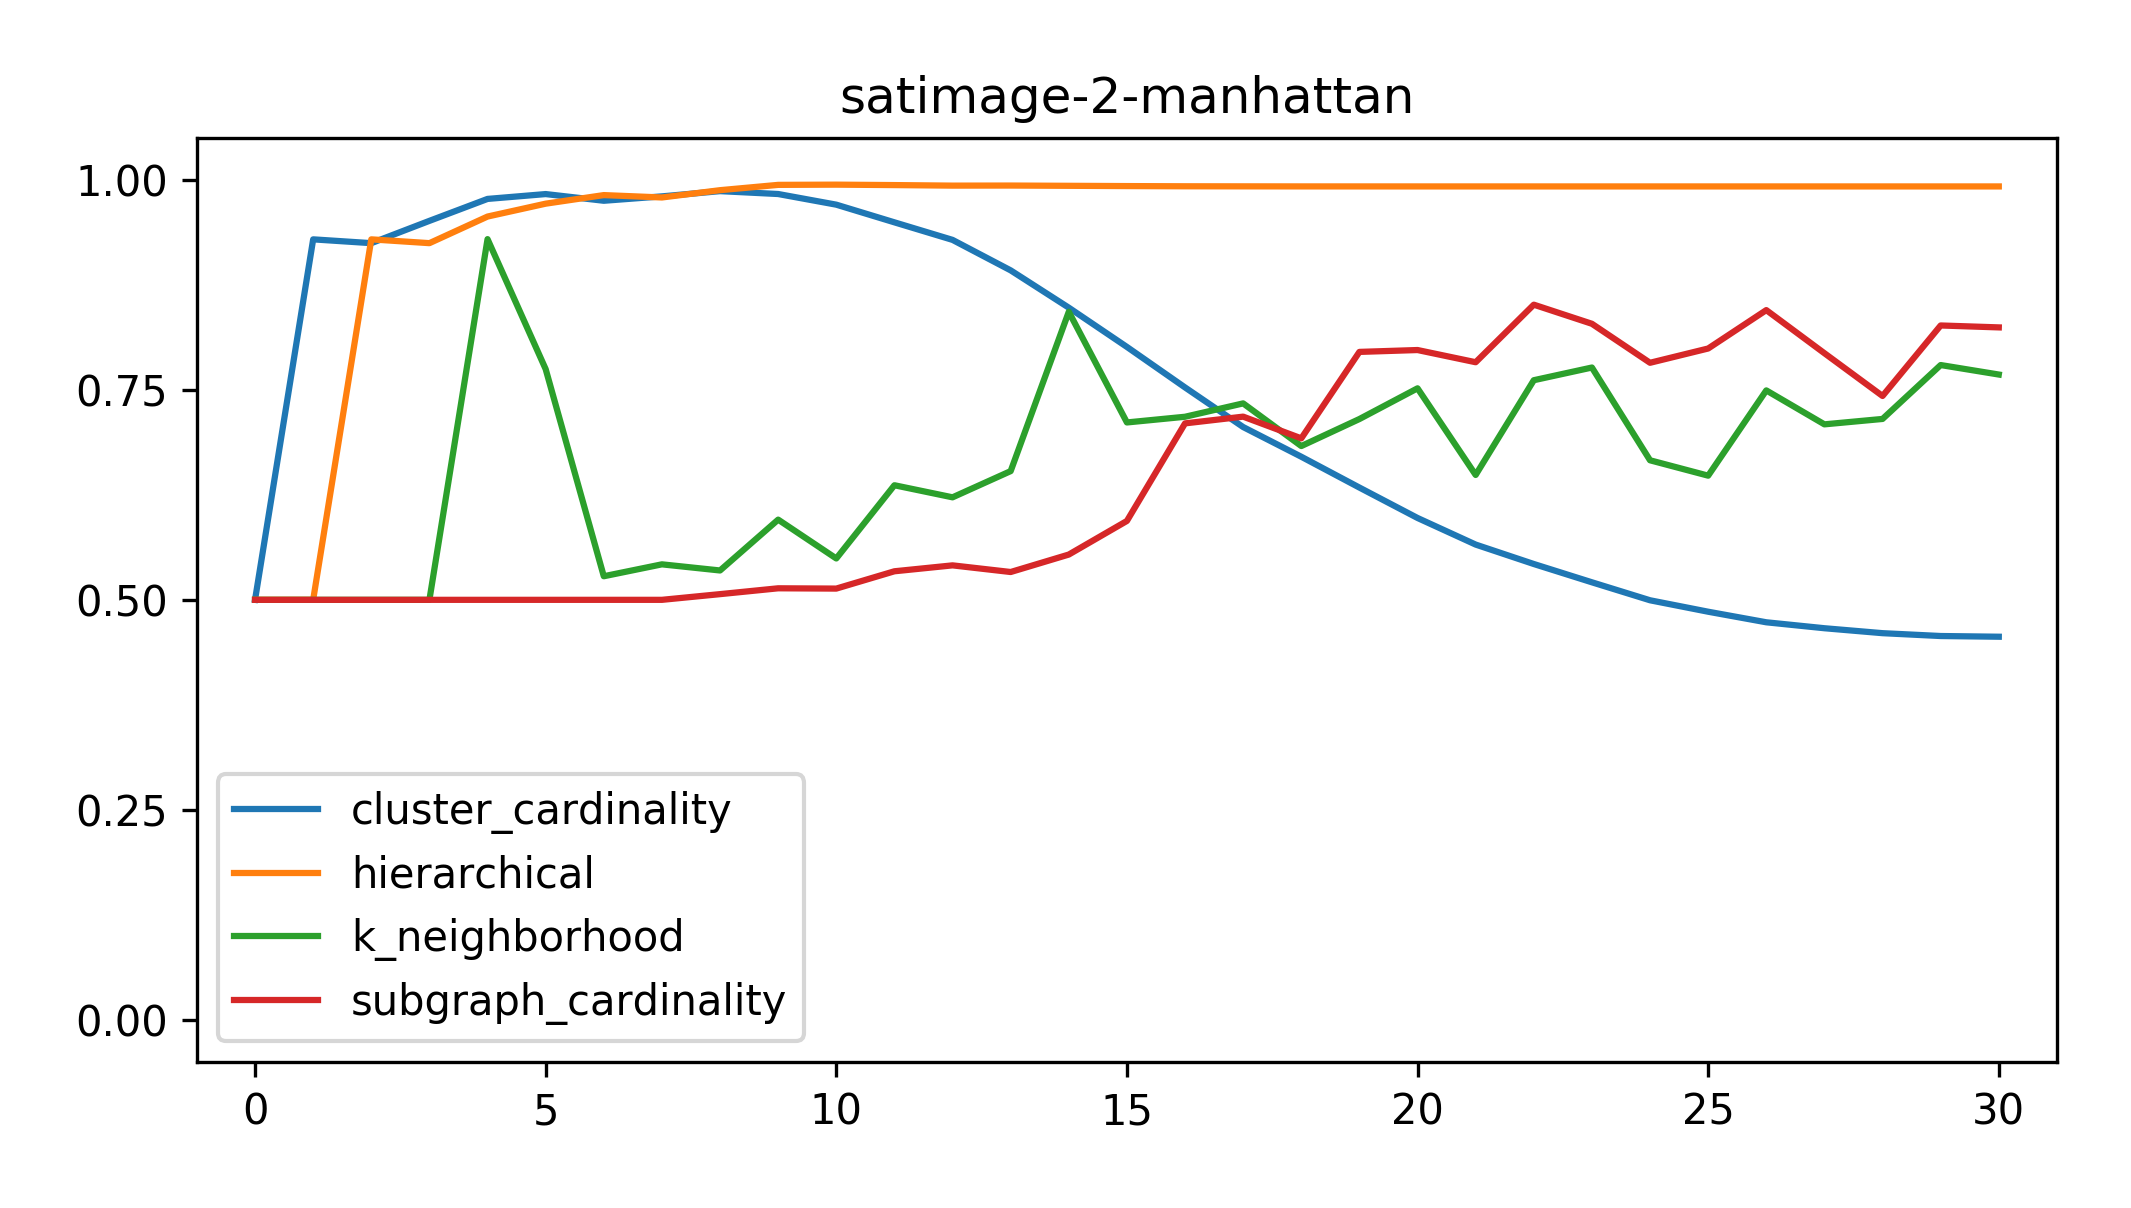
\includegraphics[width=2.2in]{kdd/static/auc_vs_depth/satimage-2-manhattan.png}

% Thyroid
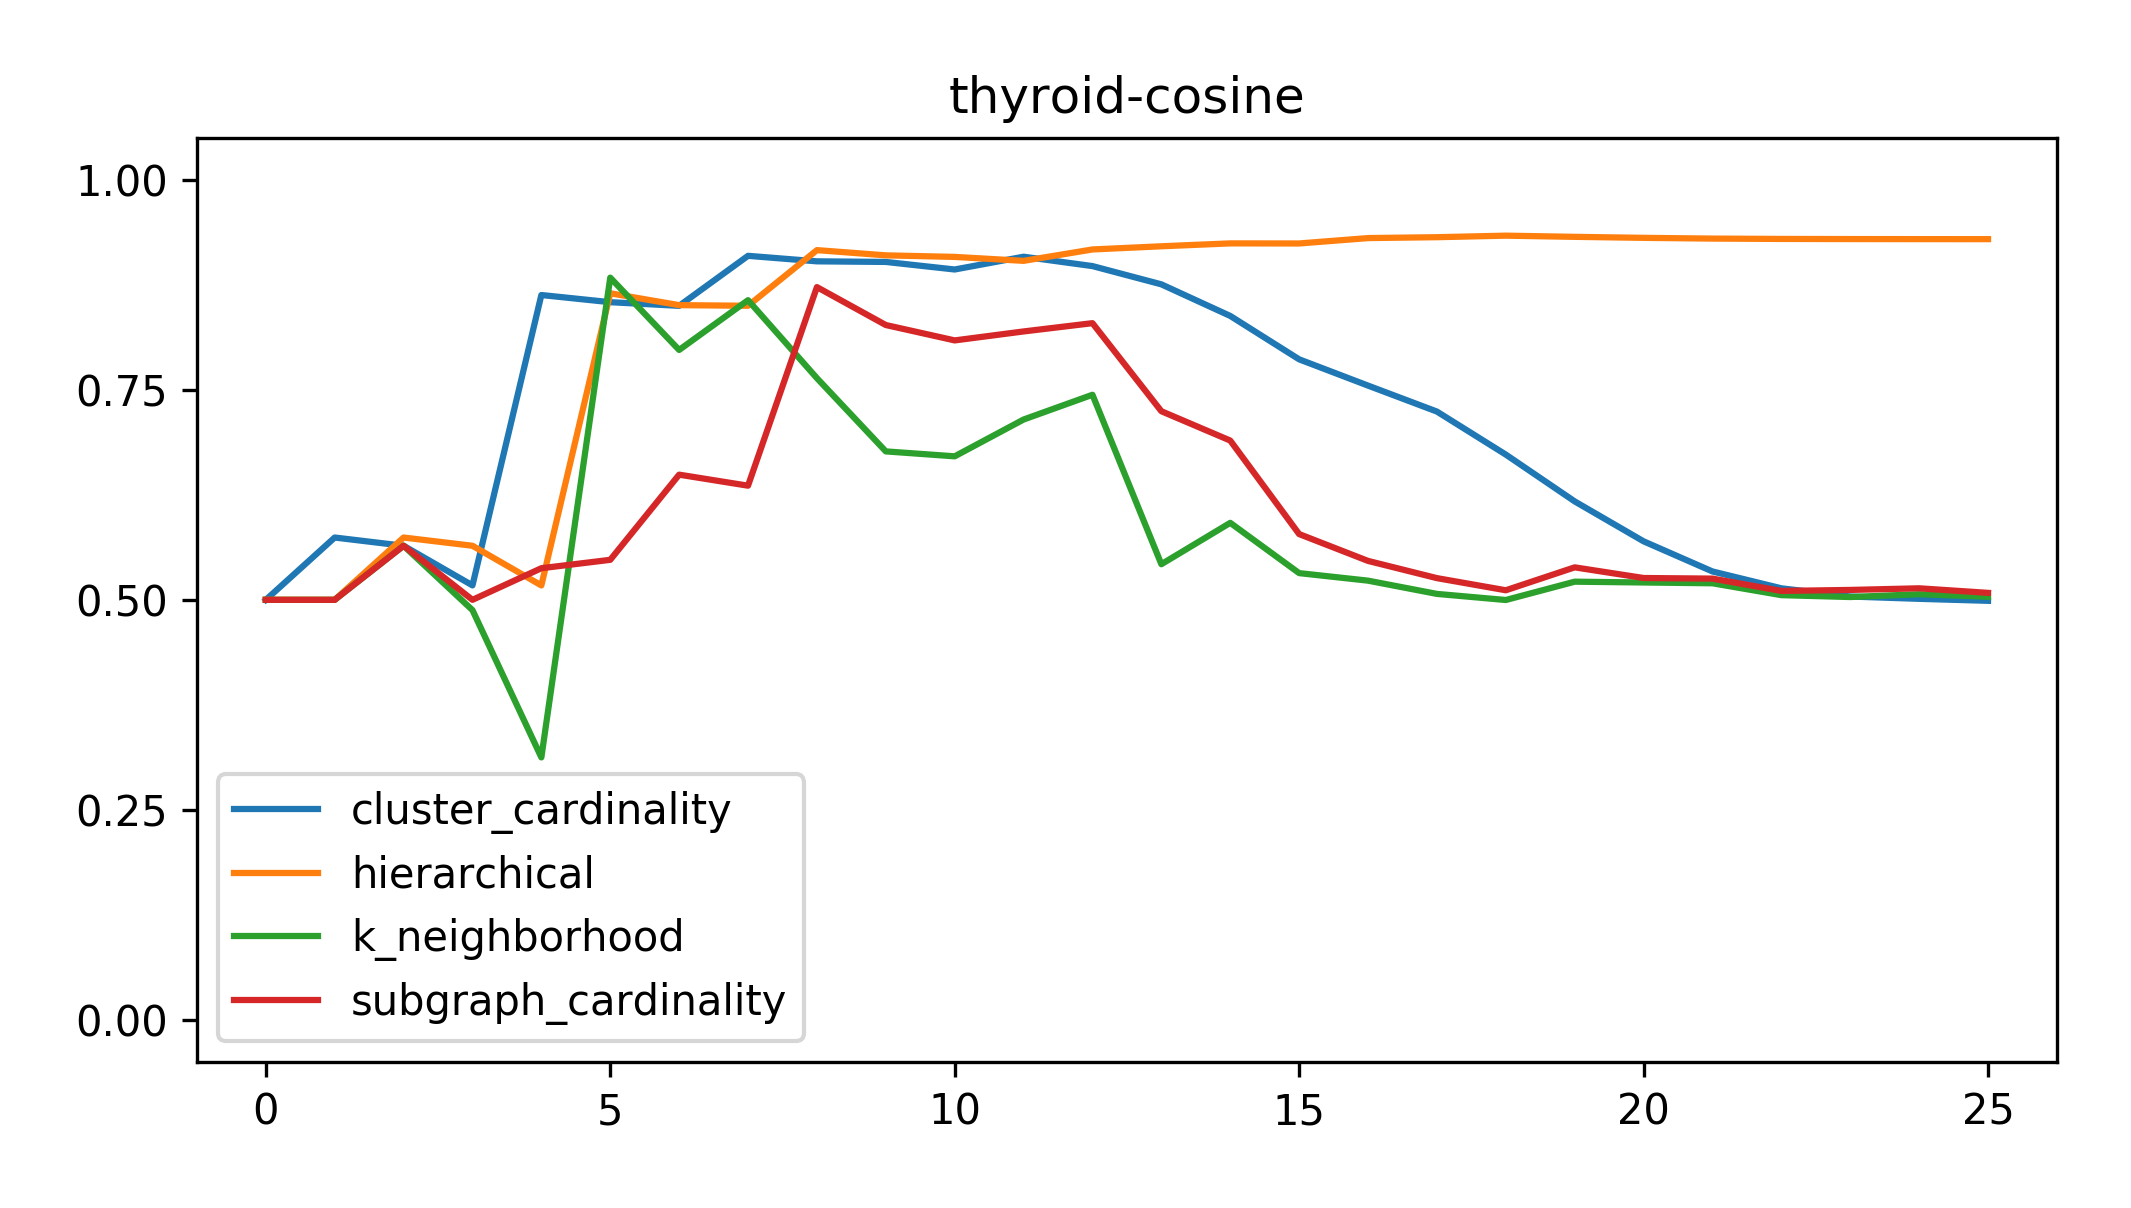
\includegraphics[width=2.2in]{kdd/static/auc_vs_depth/thyroid-cosine.png}
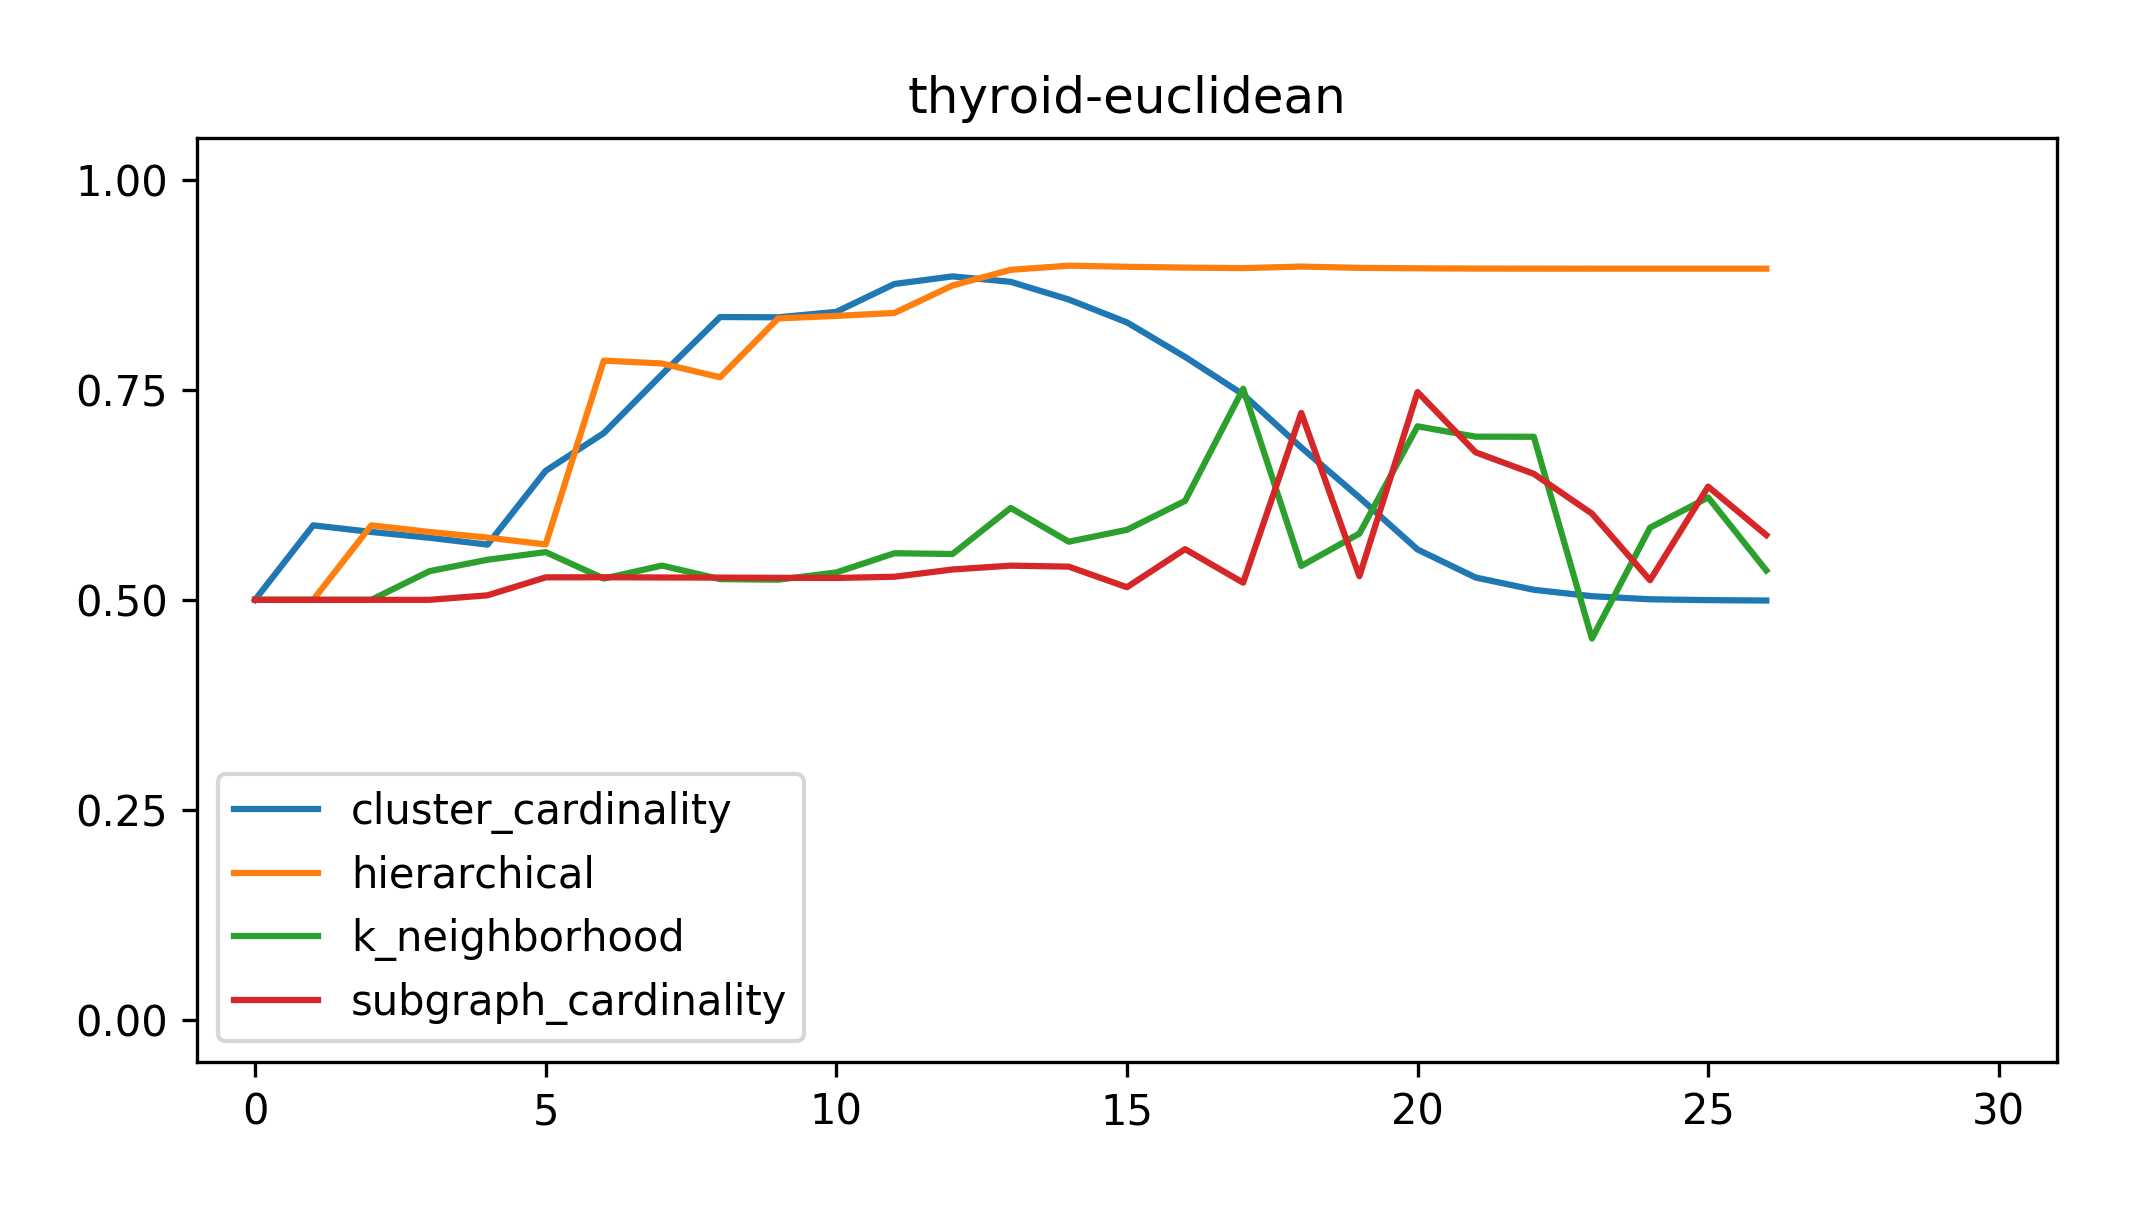
\includegraphics[width=2.2in]{kdd/static/auc_vs_depth/thyroid-euclidean.png}
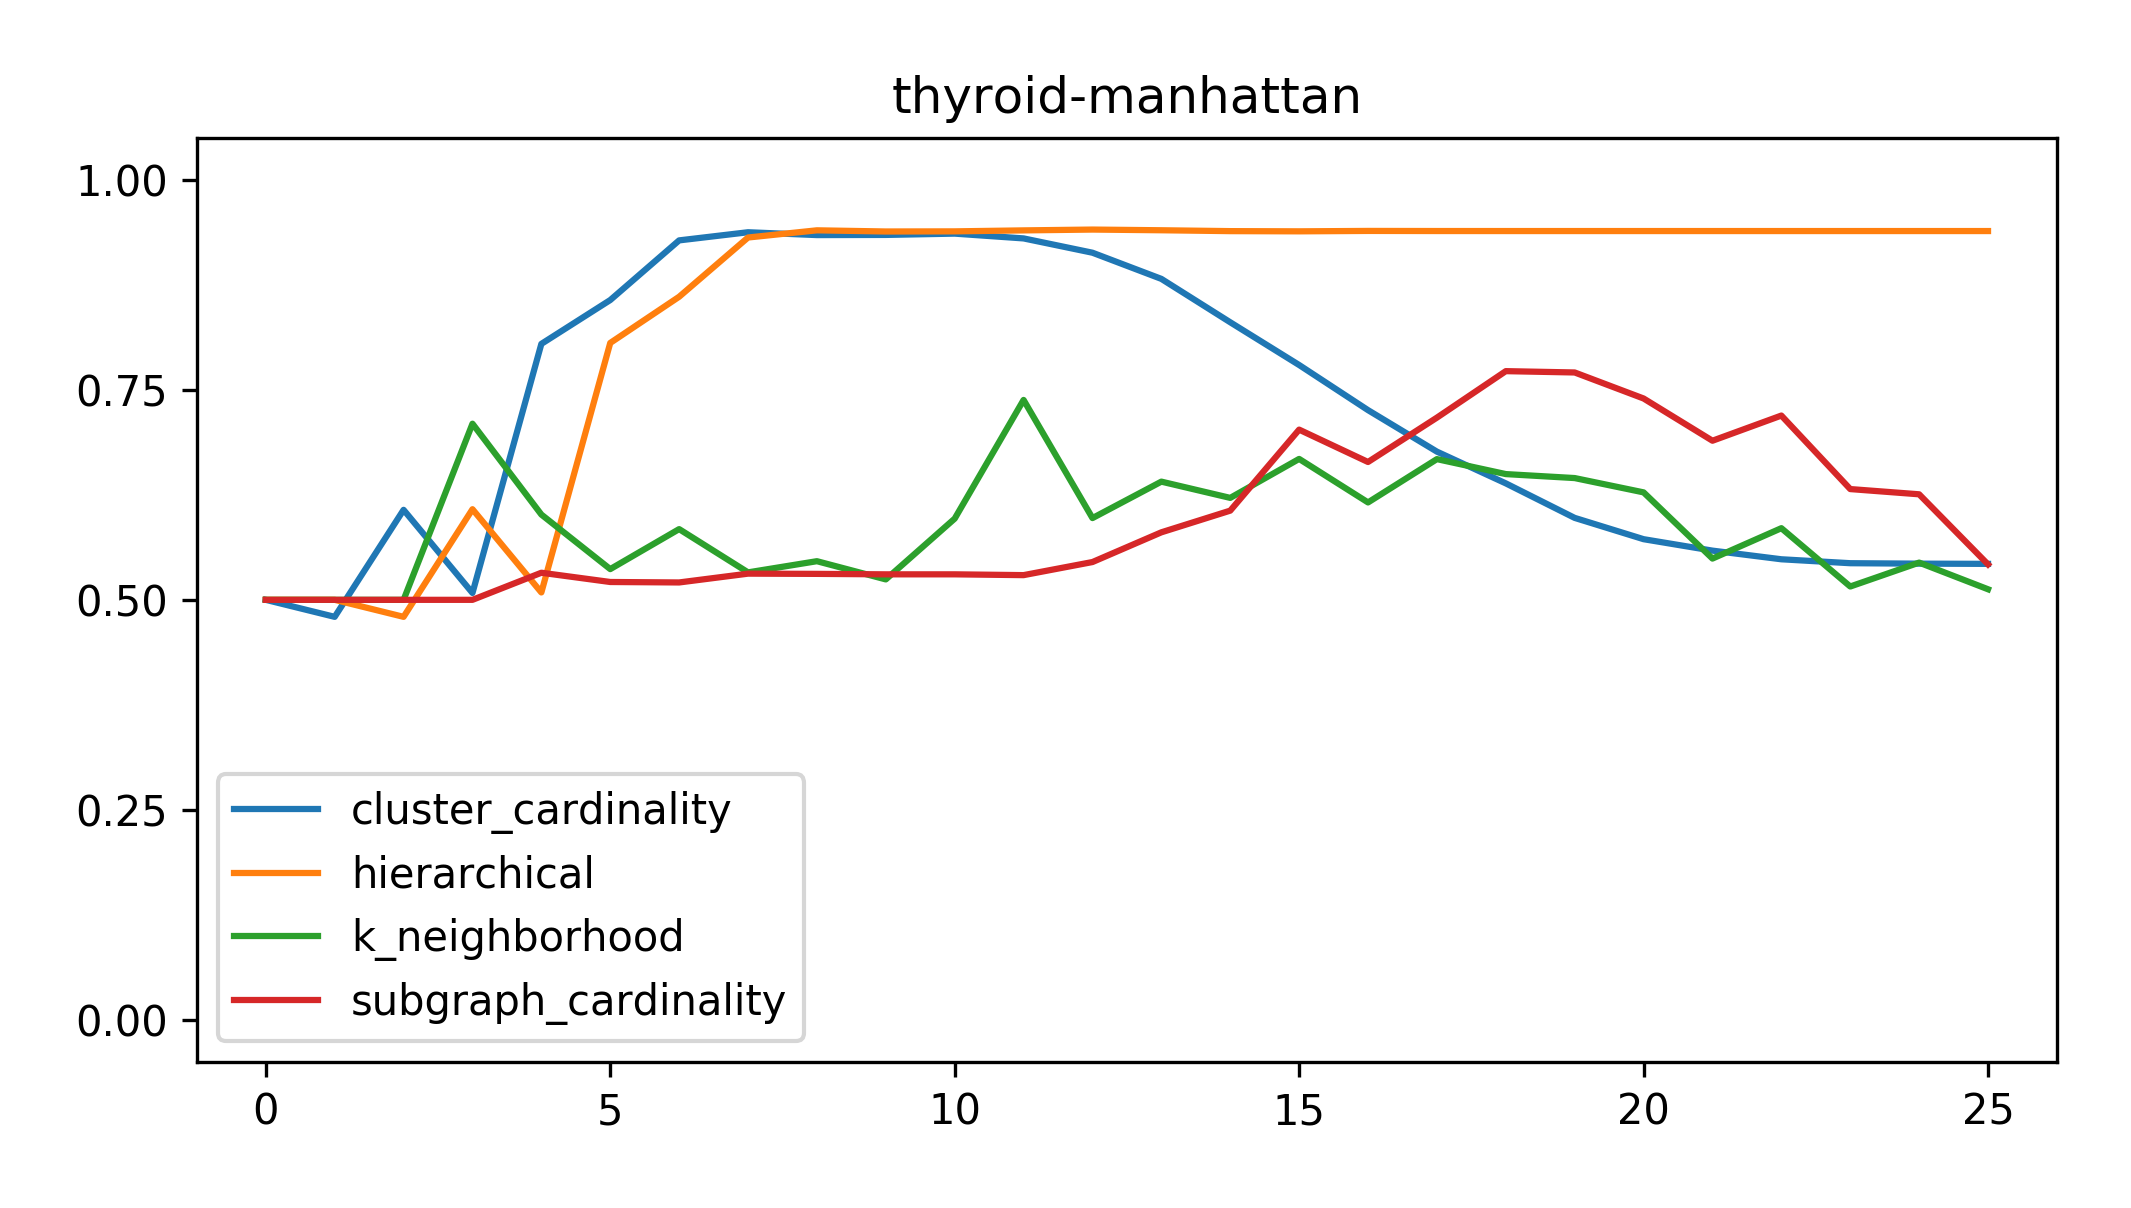
\includegraphics[width=2.2in]{kdd/static/auc_vs_depth/thyroid-manhattan.png}

% Vertebral
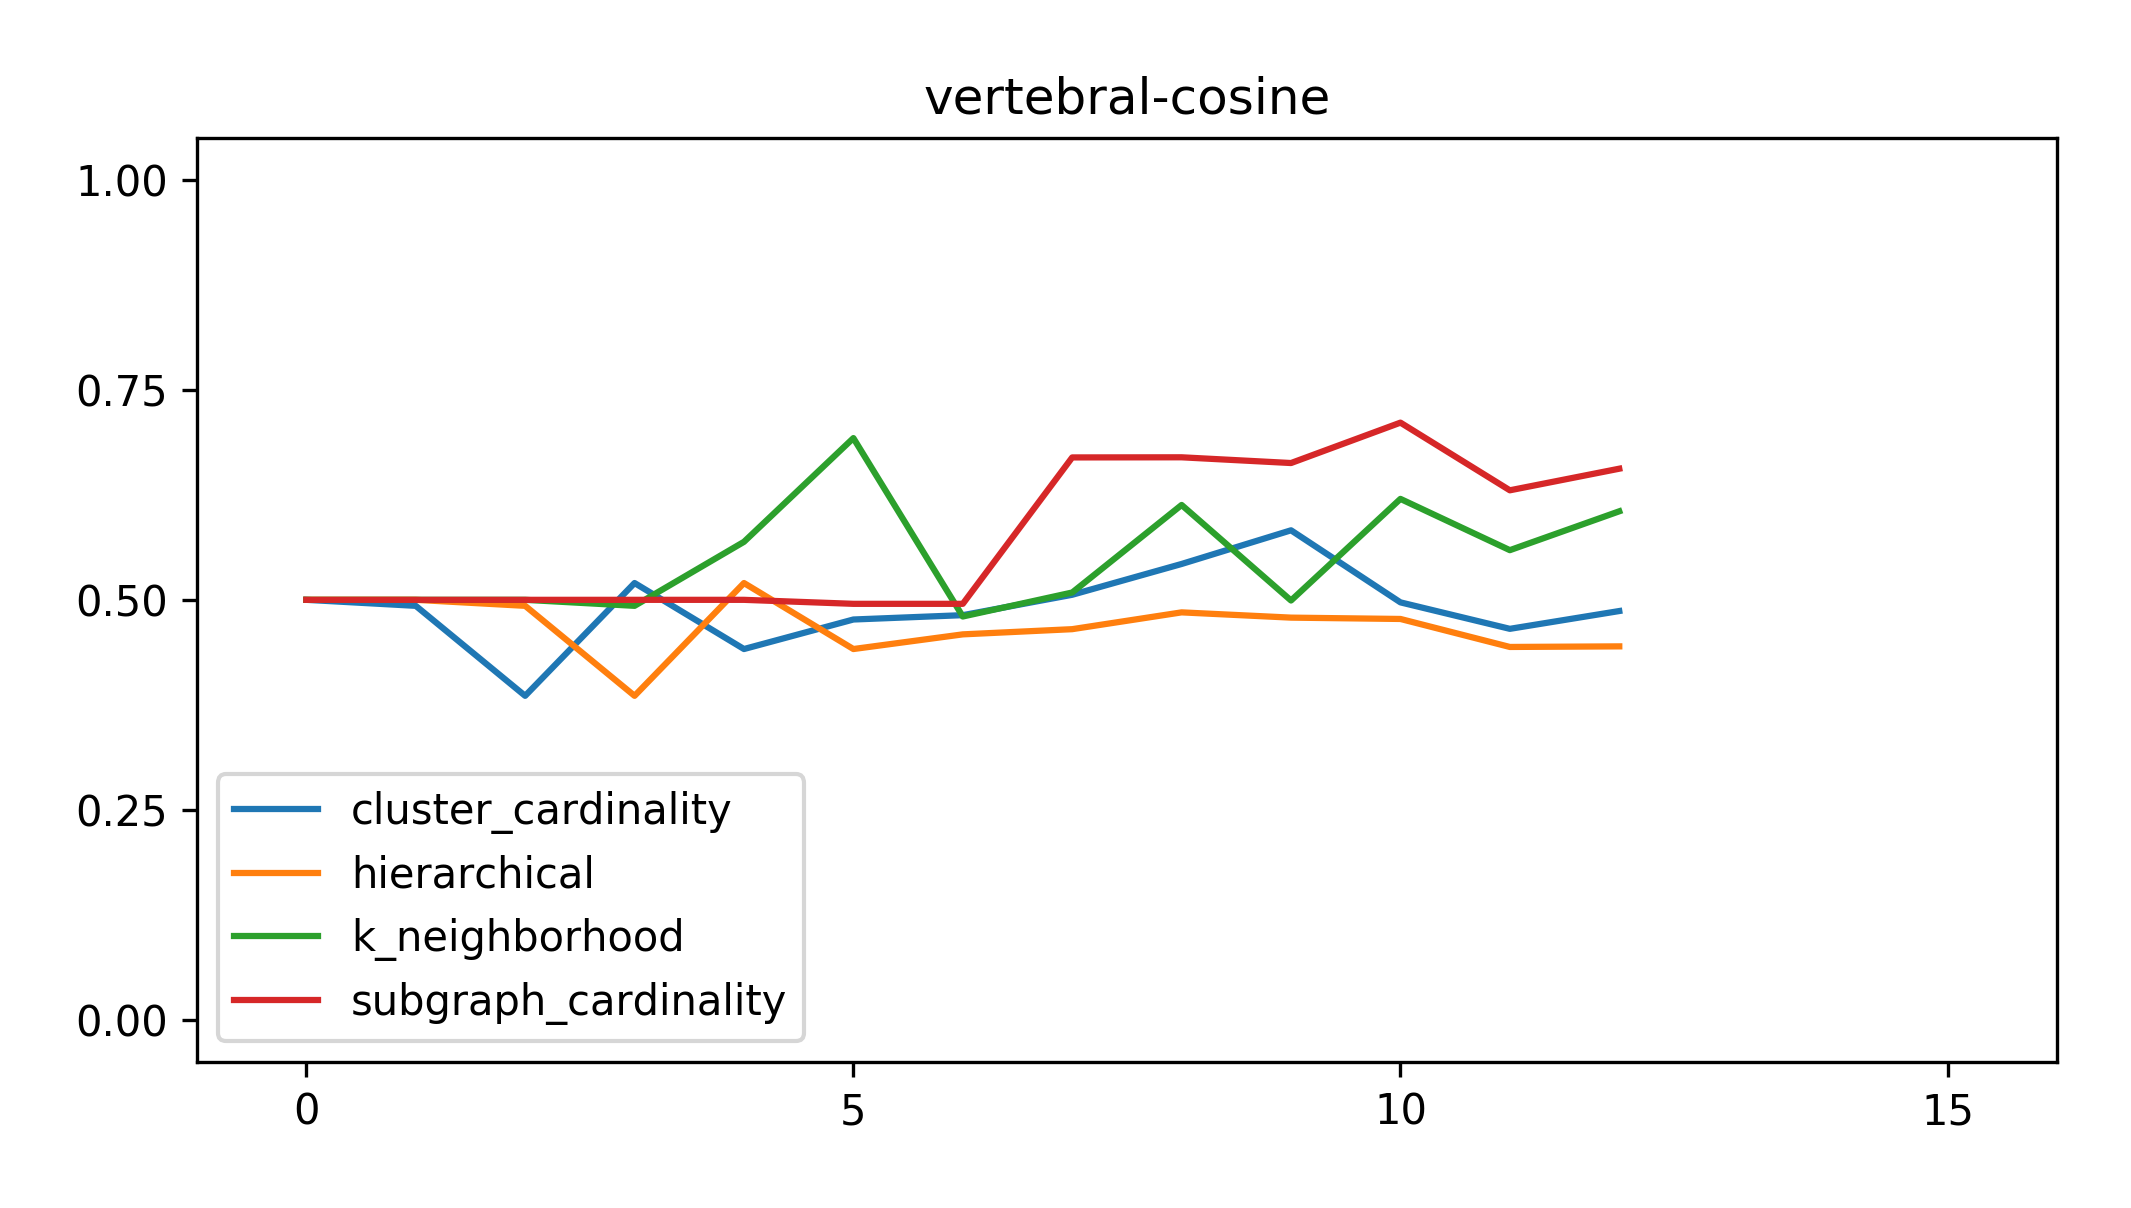
\includegraphics[width=2.2in]{kdd/static/auc_vs_depth/vertebral-cosine.png}
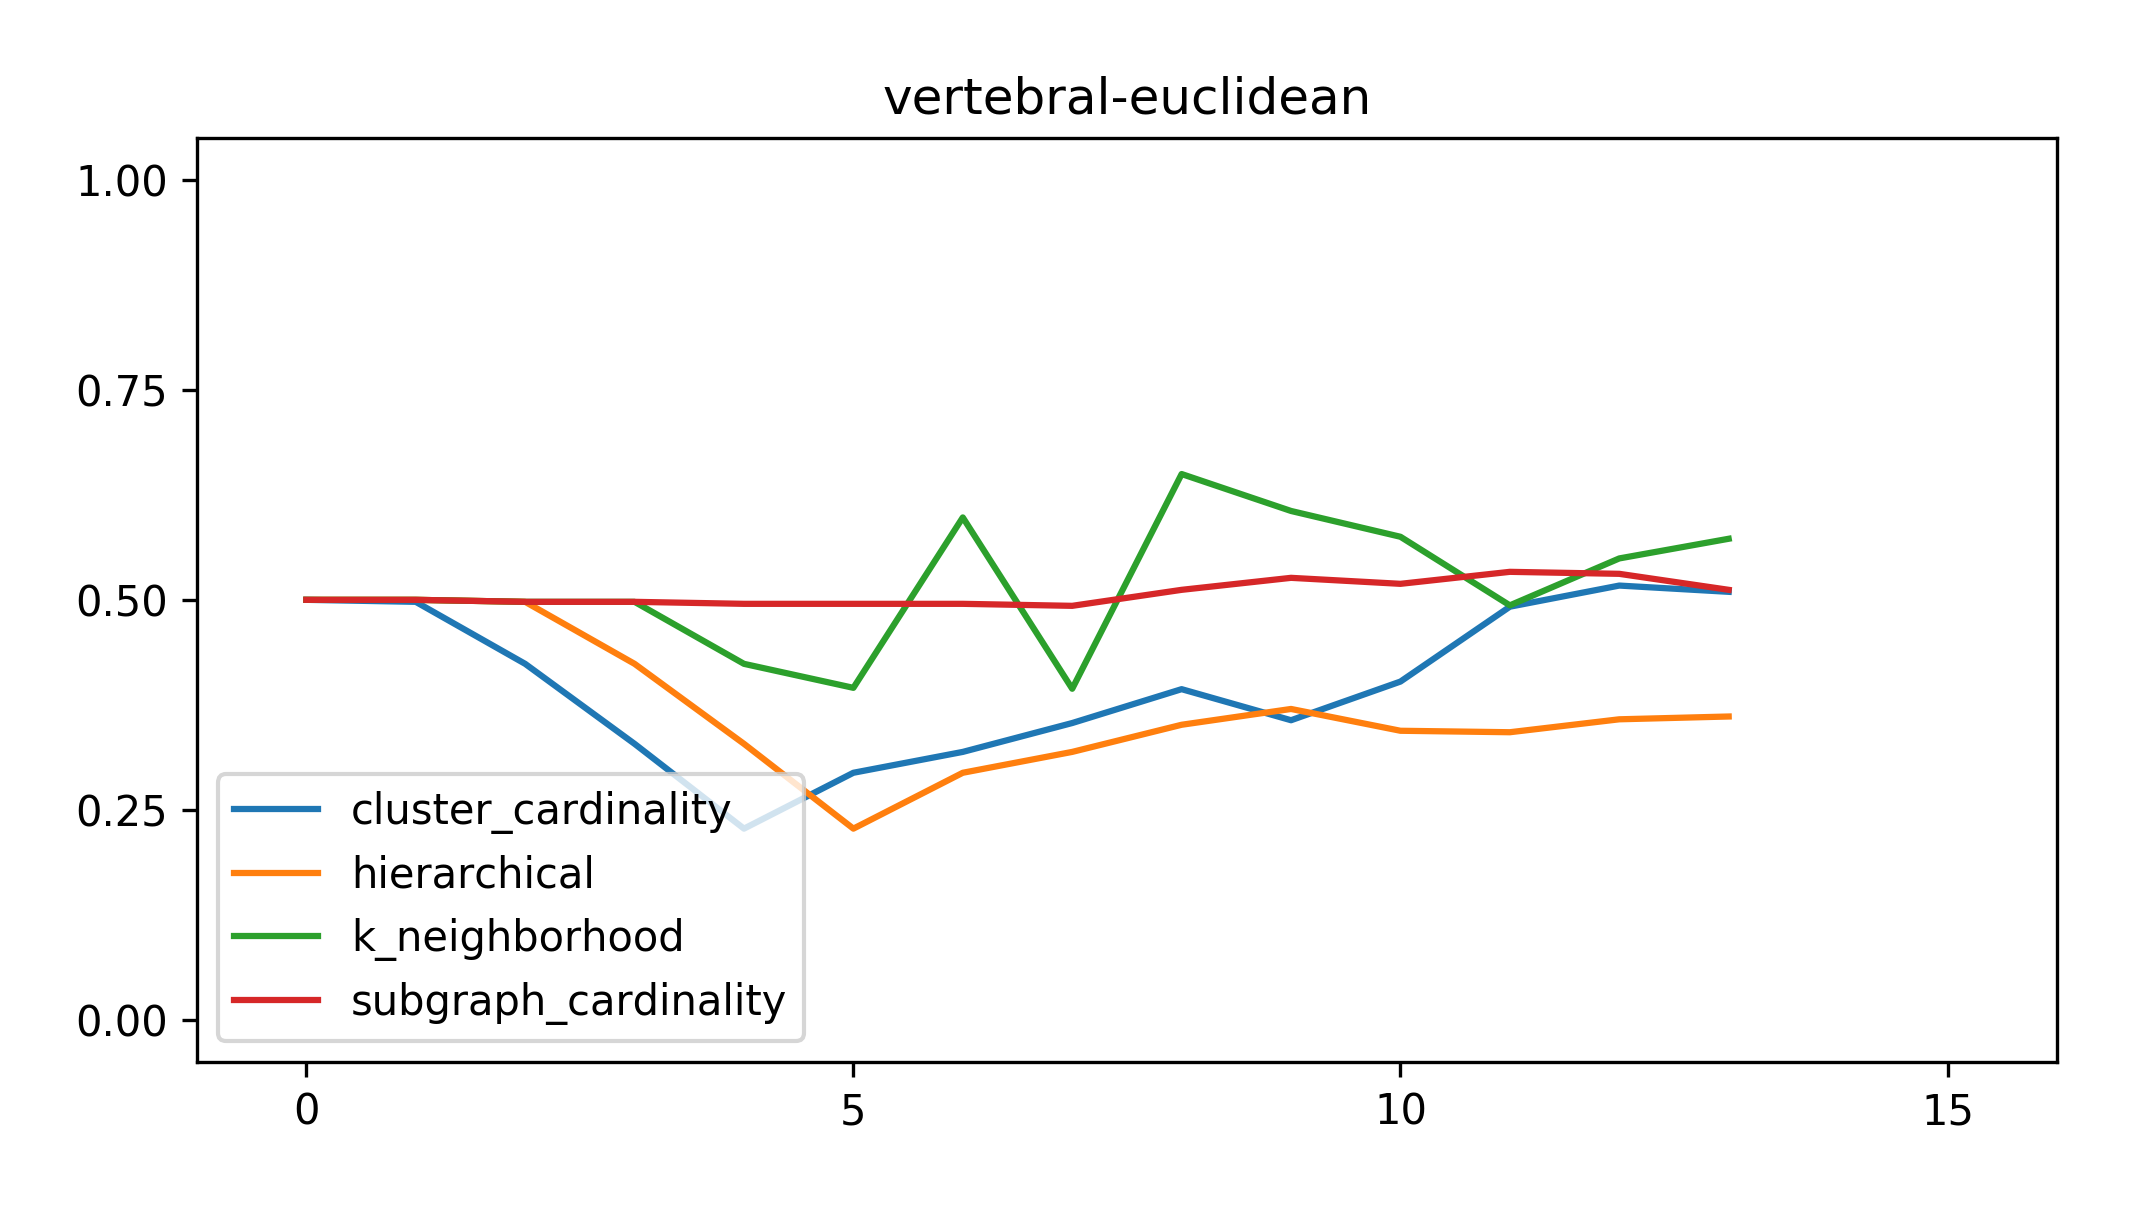
\includegraphics[width=2.2in]{kdd/static/auc_vs_depth/vertebral-euclidean.png}
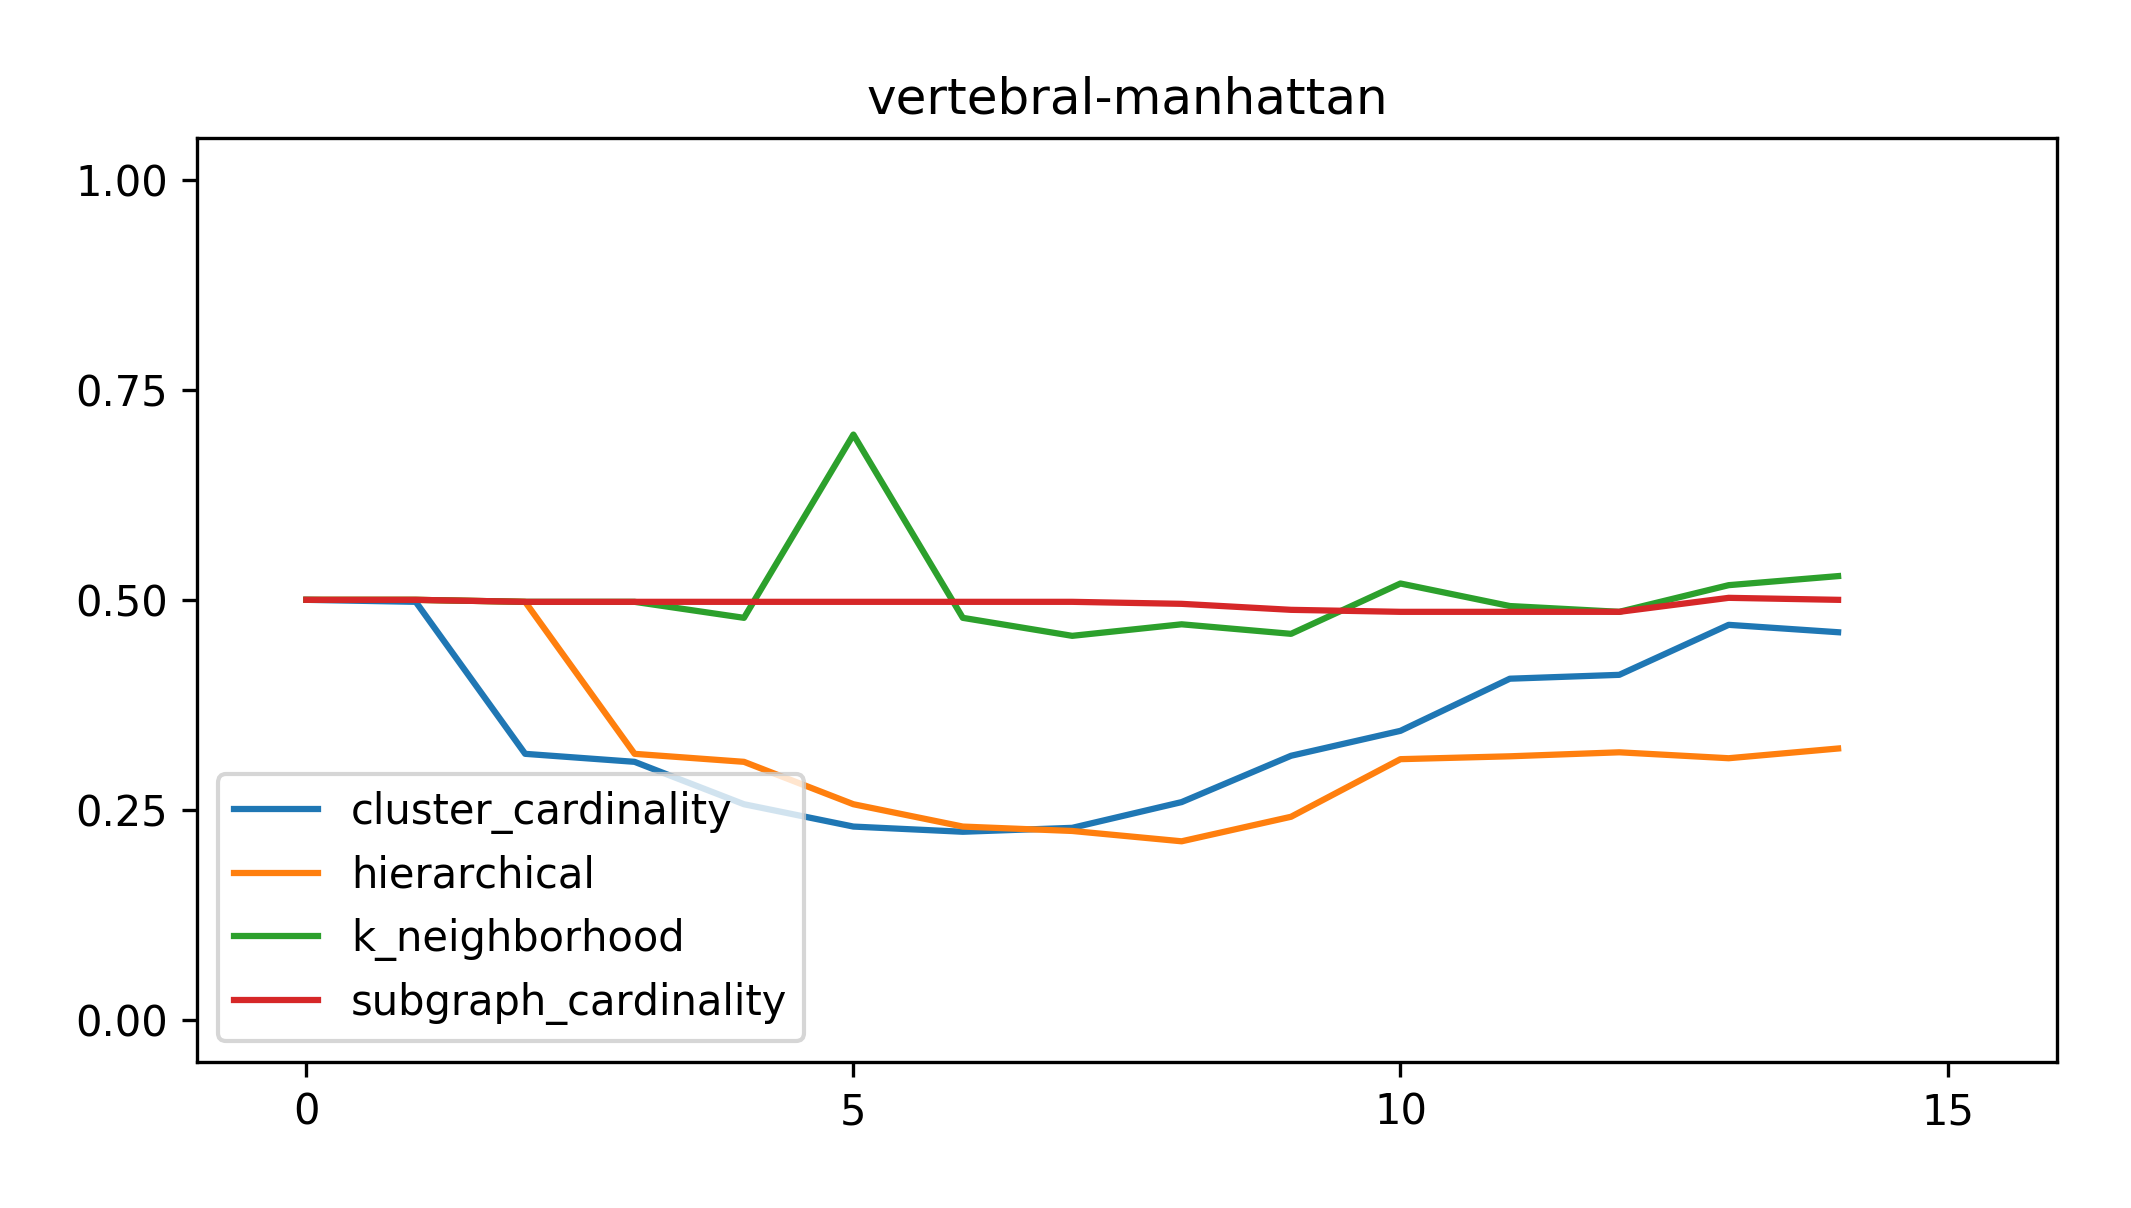
\includegraphics[width=2.2in]{kdd/static/auc_vs_depth/vertebral-manhattan.png}

% Vowels
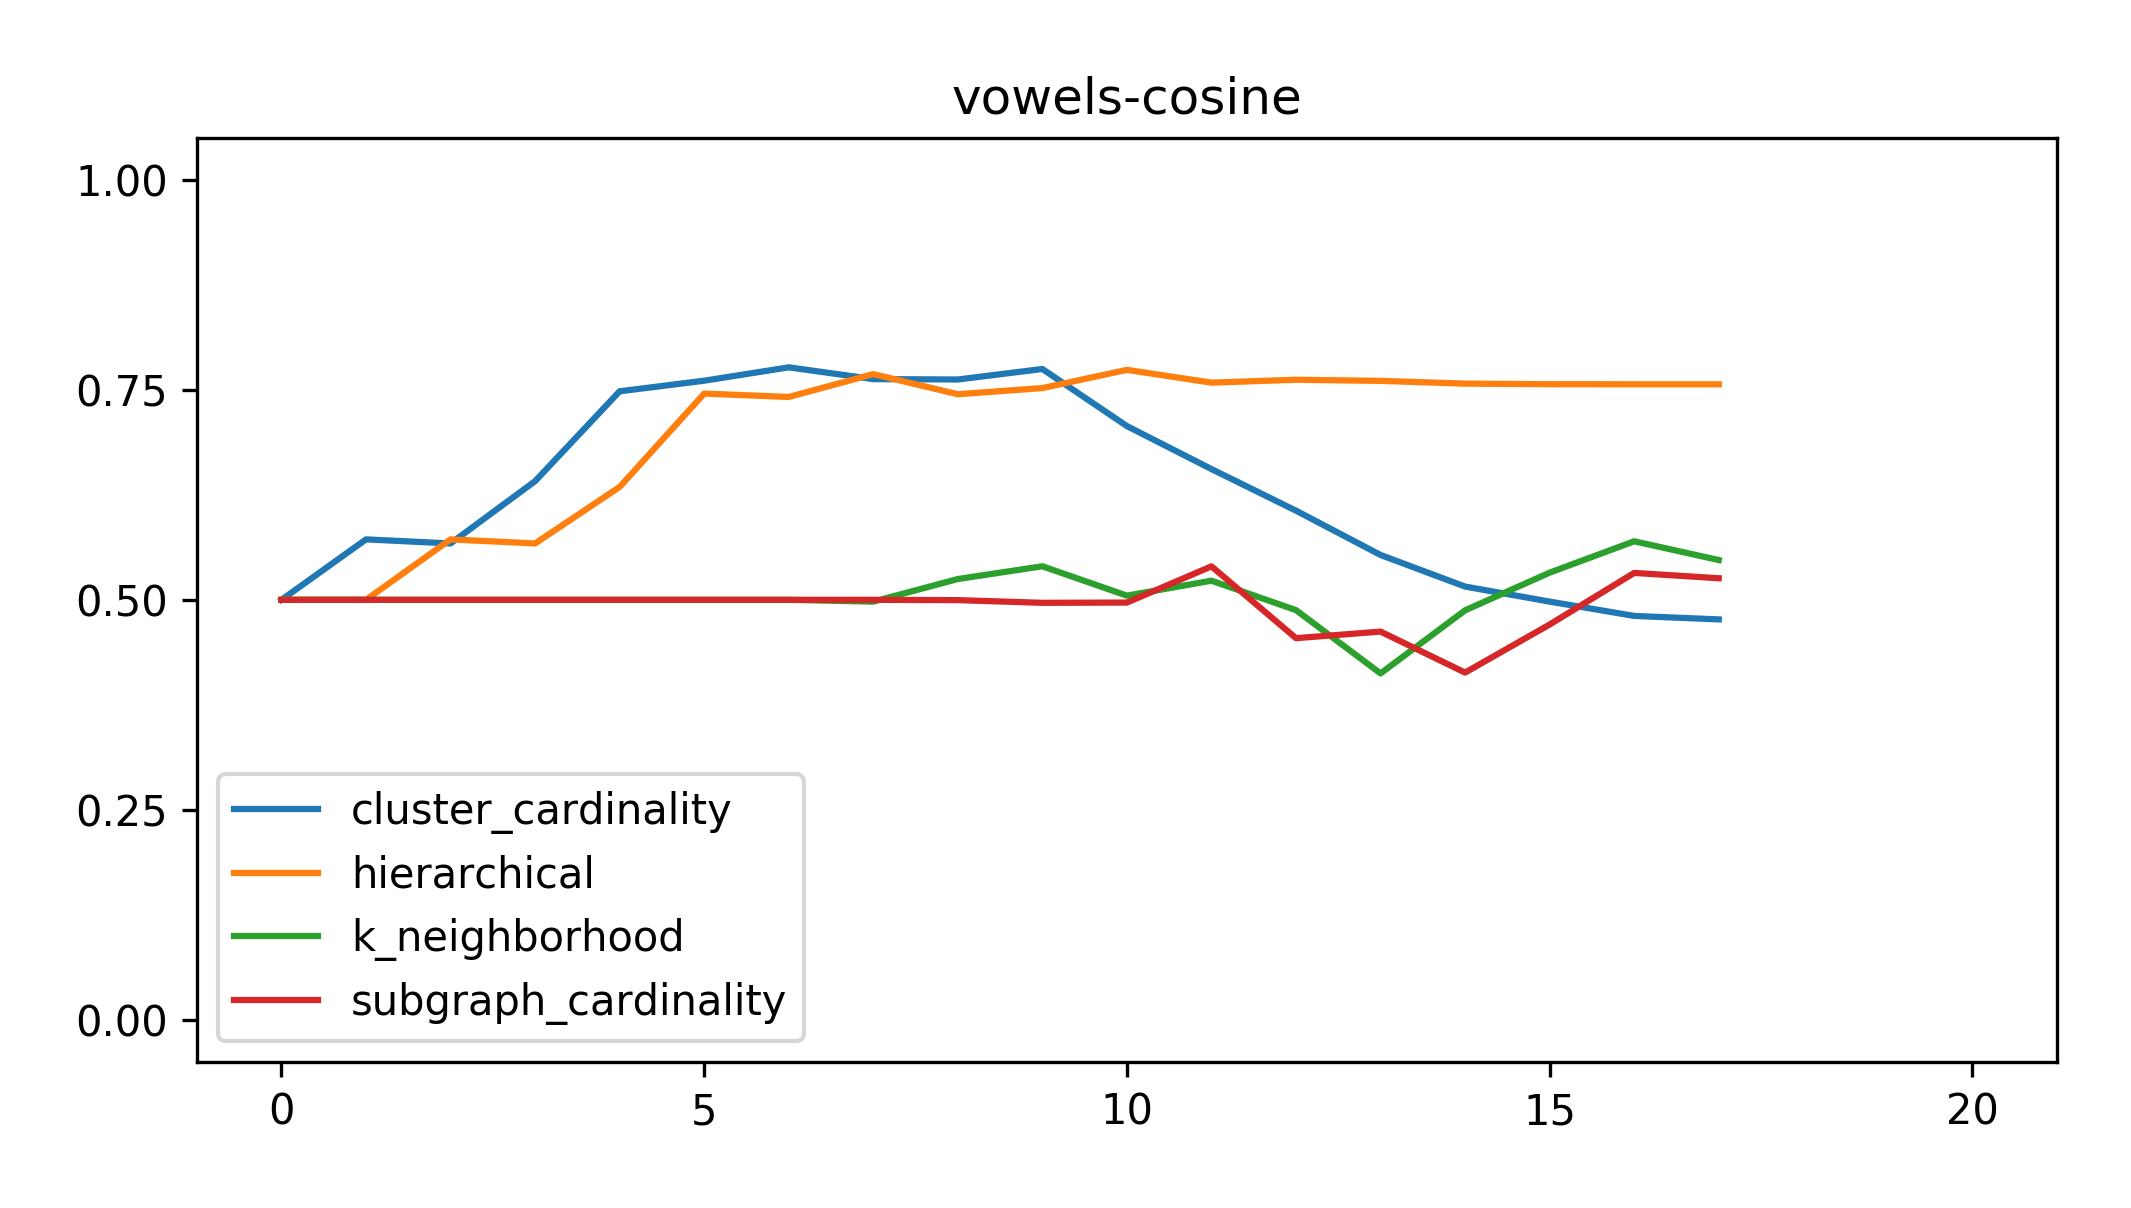
\includegraphics[width=2.2in]{kdd/static/auc_vs_depth/vowels-cosine.png}
\includegraphics[width=2.2in]{kdd/static/auc_vs_depth/vowels-euclidean.png}
\includegraphics[width=2.2in]{kdd/static/auc_vs_depth/vowels-manhattan.png}

% WBC
\includegraphics[width=2.2in]{kdd/static/auc_vs_depth/wbc-cosine.png}
\includegraphics[width=2.2in]{kdd/static/auc_vs_depth/wbc-euclidean.png}
\includegraphics[width=2.2in]{kdd/static/auc_vs_depth/wbc-manhattan.png}

% Wine
\includegraphics[width=2.2in]{kdd/static/auc_vs_depth/wine-cosine.png}
\includegraphics[width=2.2in]{kdd/static/auc_vs_depth/wine-euclidean.png}
\includegraphics[width=2.2in]{kdd/static/auc_vs_depth/wine-manhattan.png}

% HTTP
\includegraphics[width=2.2in]{kdd/static/auc_vs_depth/http-cosine.png}
\includegraphics[width=2.2in]{kdd/static/auc_vs_depth/http-euclidean.png}
\includegraphics[width=2.2in]{kdd/static/auc_vs_depth/http-manhattan.png}

\caption{
Plots of ROC-AUC vs Depth for our mearures of Anomolousness.
}

\label{results:datasets_3}
\end{figure*}

\begin{figure*}[!t]
\centering
% SMTP
\includegraphics[width=2.2in]{kdd/static/auc_vs_depth/smtp-cosine.png}
\includegraphics[width=2.2in]{kdd/static/auc_vs_depth/smtp-euclidean.png}
\includegraphics[width=2.2in]{kdd/static/auc_vs_depth/smtp-manhattan.png}

% Pendigits
\includegraphics[width=2.2in]{kdd/static/auc_vs_depth/pendigits-cosine.png}
\includegraphics[width=2.2in]{kdd/static/auc_vs_depth/pendigits-euclidean.png}
\includegraphics[width=2.2in]{kdd/static/auc_vs_depth/pendigits-manhattan.png}

% Mammography
\includegraphics[width=2.2in]{kdd/static/auc_vs_depth/mammography-cosine.png}
\includegraphics[width=2.2in]{kdd/static/auc_vs_depth/mammography-euclidean.png}
\includegraphics[width=2.2in]{kdd/static/auc_vs_depth/mammography-manhattan.png}

\caption{
Plots of ROC-AUC vs Depth for our mearures of Anomolousness.
}

\label{results:datasets_4}
\end{figure*}



% \clearpage
\section{Conclusions}
\label{sec:conclusions}

We conclude that Manifold Learning via CHESS lays a strong foundation for both introspective and online anomaly detection.
The clustering mechanism faithfully maps the underlying manifold, given the proper stopping conditions.

Future works in this area should examine more novel stopping criteria, specifically ones that allow automated manifold detection.
Additionally, work should be carried out to examine how this technique scales to higher dimensional data and how different distance functions impact performance.

In this paper, we have cleared the way for work towards automated manifold detection, introspective and online anomaly detection, and the novel concept of depth-wise graphs within the manifold itself.

\bibliographystyle{ACM-Reference-Format}
\bibliography{references}
\end{document}
